\documentclass[12pt]{article}
% Language setting
\usepackage[english]{babel}
\usepackage{graphics}
\usepackage[draft]{graphicx}
\usepackage{fancyhdr} 
\usepackage{placeins}

% Set page size and margins
% Replace `letterpaper' with `a4paper' for UK/EU standard size

\usepackage[a4paper,top=2.0cm,bottom=2.54cm,left=3cm,right=2cm,marginparwidth=1.75cm]{geometry}

\usepackage{tocloft}
\usepackage[utf8]{inputenc}
\usepackage[T1]{fontenc}
\usepackage{lmodern} %change the name in the brackets in order to change the 
\renewcommand*\familydefault{\sfdefault}  %% Only if the base font of the document is to be sans serif

% Useful packages
\usepackage{amsmath}

\usepackage{graphicx}
\usepackage[colorlinks=true, allcolors=blue]{hyperref}
\usepackage{float}
\usepackage{algorithm}
\usepackage{algpseudocode}
\usepackage{pifont}
\usepackage{setspace} 
\usepackage{caption}
\usepackage[flushleft]{threeparttable}
\usepackage[titletoc]{appendix}
\usepackage[intoc]{nomencl}
\usepackage{multicol}
\usepackage{ifthen}
  \renewcommand{\nomgroup}[1]{%
  \item[\bfseries
  \ifthenelse{\equal{#1}{P}}{Greek}{%
  \ifthenelse{\equal{#1}{O}}{Non-Dimensional Numbers}{%
  \ifthenelse{\equal{#1}{L}}{Latin}{%
  \ifthenelse{\equal{#1}{N}}{Subscripts/ Superscripts }{}}}}%
  ]}
  \renewcommand*\nompreamble{\begin{multicols}{2}}
    \renewcommand*\nompostamble{\end{multicols}}

 % Set line spacing to 1.5
%\renewcommand{\bibname}{References} %to change the reference title



%-------------------------BEGIN DOCUMENT----------------------------------%
\numberwithin{equation}{section}
% \renewcommand{\theequation}{\arabic{section}.\arabic{equation}} 
\begin{document}
\begin{titlepage}
\title{Optimized Condensation for Energy Storage:
Thermodynamics and Modeling}
\author{Omry Magen}

\newcommand{\HRule}{\rule{\linewidth}{0.5mm}} % Defines a new command for the horizontal lines, change thickness here

%----------------------------------------------------------------------------------------
%	LOGO SECTION
%----------------------------------------------------------------------------------------

% 
\includegraphics[width=8cm]{Figures/Logo.png}\\[1cm] 
 
%----------------------------------------------------------------------------------------

\center % Center everything on the page

%----------------------------------------------------------------------------------------
%	HEADING SECTIONS
%----------------------------------------------------------------------------------------

\vspace*{3cm}
\textsc{\Large Imperial College London}\\[1.5cm] % Major heading such as course name
\textsc{\large Department of Mechanical Engineering}\\[0.5cm] % Minor heading such as course title
\textsc{\large Advanced Mechanical Engineering Course}\\[1.5cm] % Name of your university/college

%----------------------------------------------------------------------------------------
%	TITLE SECTION
%----------------------------------------------------------------------------------------
\makeatletter

{ \huge \bfseries \@title}\\[1cm] % Title of your document

 
%----------------------------------------------------------------------------------------
%	AUTHOR SECTION
%----------------------------------------------------------------------------------------




\begin{minipage}{0.4\textwidth}
\centering \large
By:\\
\@author % Your name            
\end{minipage}\\[0.1cm]


\begin{minipage}{0.4\textwidth}
\centering \large
BSc. Mechanical Engineering at Technical University Berlin \\[1.2em] % Supervisor's Name           
\end{minipage}\\[1cm]
\makeatother % If you don't want a supervisor, uncomment the two lines below and remove the section above       
 % \Large\@author\\[3cm] % Your name                %----------------------------------------------------------------------------------------        %    DATE SECTION        %---------------------------------------------------------------------------------------- 
 \begin{minipage}{1\textwidth}
    \centering \large
    A thesis submitted in partial fulfillment of the requirements for the Master of Science Degree of  Imperial College London and the Diploma of Membership of Imperial College \\[0.9cm] 
    {\today}\\[0.1cm] 
    \begin{center}
        Word Limit: 18,000\\
        Word Count: 16,240     
    \end{center}
\end{minipage}\\ 
                  
 % Date, change the \today to a set date if you want to be precise 
% \vspace*{\fill}




\makeatother
 % Fill the rest of the page with whitespace

\end{titlepage} 
\newpage

\addcontentsline{toc}{section}{Abstract}

\pagenumbering{Roman}
\setcounter{page}{2}

\section*{Abstract}

This research project investigates the phenomenon of condensation in both homogeneous and heterogeneous conditions and a numerical model to simulate dropwise condensation found within condensers is proposed. Initially, a novel model was developed to describe droplet condensation in air-vapor mixtures. The new model is constructed based on the established $d^{2}$ evaporation law, with boundary conditions reversed and guided by the Kelvin equation to represent the condensation process. The $d^{2}$ model was comprehensively compared with existing models describing droplet condensation in pure vapor found in the literature. The findings indicate that the $d^{2}$ model exhibits physically realistic behavior and qualitative alignment with the existing models under similar conditions.

Furthermore, a parametric analysis was conducted for heterogeneous droplet growth. A heat transfer model was adopted from prior research. This model was based on a specific mode of heterogeneous condensation, namely dropwise condensation, as it holds favorable heat transfer properties and remains a highly researched topic to this day. Critical parameters of this model were identified and displayed strong agreement with existing literature. The iterative solutions to the droplet growth models were implemented using Python code.

Subsequently, nucleation and droplet growth models for homogeneous conditions were implemented in a solver using an Eulerian/Eulerian approach within the OpenFOAM framework. Transport equations and their respective source terms based on relevant literature were consistently adopted. These models were acquired from studies simulating the homogeneous condensation phenomenon within steam turbines. A 2D cylinder case was studied, yielding physically meaningful results. It was concluded that this code's simplicity and efficiency make it a suitable tool for modeling heterogeneous cases as well.

Dropwise heterogeneous condensation, previously deemed not feasible for CFD methods, was modeled under similar principles used for the homogeneous case. Source terms and other simulation parameters were adjusted to suit the new conditions. A simple flat plate case was simulated to obtain quantitative data regarding wall heat flux. A droplet size distribution model from the literature was utilized and it was found that meeting a strong assumption regarding the droplet growth rate yielded good agreement with existing models. The results effectively replicated established trends, affirming that an Eulerian/Eulerian method can serve as a valuable tool for simulating dropwise condensation and potential enhancements to the proposed model were then discussed. The proposed numerical model's capacity to efficiently replicate wall heat flux values across diverse conditions could serve as a valuable tool for analyzing condenser flow dynamics, thereby facilitating optimization strategies.


\newpage
\addcontentsline{toc}{section}{Acknowledgements}
\section*{Acknowledgements}
I wish to convey my profound appreciation to Dr. Andrea Giusti, who has diligently overseen this project over the course of the year. I am immensely grateful for the invaluable time, guidance, enthusiasm, and humor you have consistently shared with me each week. It has undeniably been the most enriching and progressive period of my academic journey at Imperial College. These meetings have significantly broadened my horizons in the realm of thermofluids and my overall development as a mechanical engineer. Your inspiration has fueled my aspirations to pursue a continued academic career.

I extend my heartfelt thanks to my friends, with whom I've had the privilege of meeting and spending my time here in London. Our adventures in Wales have created memories that will forever hold a special place in my heart. Exploring different cultures and embracing new experiences has not only been fascinating but has also contributed to my personal growth.

Lastly, I would like to express my deepest gratitude to my parents, Orly and Hillel Magen, whose unwavering support has made the past seven years in Berlin and London possible. Your boundless love and care have been a constant source of motivation, propelling me to strive for excellence in all that I do. I am acutely aware of the privilege I have in having your unconditional backing, and I will forever be indebted to you. None of my achievements would have been attainable without your support.

\newpage

\hypersetup{linkcolor=black}
\tableofcontents    



\listoffigures
\listoftables

\newpage

\makenomenclature

\nomenclature[P]{\(\rho\)}{Density, $\mathrm{kg/m^3}$}
\nomenclature[P]{\(\vartheta\)}{Cylinder Angular Coordinates, $\mathrm{deg}$}
\nomenclature[P]{\(\alpha\)}{Volumetric Phase Fraction}
\nomenclature[P]{\(\hat{\alpha}\)}{Thermal Diffusivity, $\mathrm{m^{2}/s}$}
\nomenclature[P]{\(\sigma\)}{Surface Tension, $\mathrm{N/m}$}
\nomenclature[P]{\(\lambda\)}{Thermal Conductivity, $\mathrm{W/mK}$}
\nomenclature[P]{\(\Gamma\)}{Thermal Diffusion Coefficient, $\mathrm{m^{2}/s}$}
\nomenclature[P]{\(\eta\)}{Droplet Number, $\mathrm{1/m^3}$}
\nomenclature[P]{\(\theta\)}{Contact Angle}
\nomenclature[P]{\(\mu\)}{Dynamic Viscosity, $\mathrm{Pa\cdot s}$}
\nomenclature[P]{\(\hat{\sigma}\)}{Accommodation Coefficient}
\nomenclature[P]{\(\gamma\)}{Specific Heat Ratio}
\nomenclature[P]{\(\kappa\)}{Turbulent Kinetik Energy, $\mathrm{J/kg}$}
\nomenclature[P]{\(\epsilon\)}{Turbulent Kinetik Energy Dissipation, $\mathrm{m^{2}/s}$}
\nomenclature[P]{\(\Omega\)}{Boundary Patch}
\nomenclature[P]{\(\tau\)}{Viscous Stress Tensor}
\nomenclature[L]{\(h\)}{Heat Transfer Coefficient, $\mathrm{W/m^{2}K}$}
\nomenclature[L]{\(r\)}{Radius, $\mathrm{m}$}
\nomenclature[L]{\(T\)}{Temperature, $\mathrm{K}$}
\nomenclature[L]{\(g\)}{Gravitational Acceleration, $\mathrm{m/s^{2}}$}
\nomenclature[L]{\(p\)}{Pressure, $\mathrm{Pa}$}
\nomenclature[L]{\(R\)}{Gas Constant, $\mathrm{J/kgK}$}
\nomenclature[L]{\(J\)}{Nucleation Rate, $\mathrm{1/m^{3}s}$}
\nomenclature[L]{\(F\)}{Gibbs Free Energy, $\mathrm{J}$}
\nomenclature[L]{\(k_{B}\)}{Boltzmann Constant, $\mathrm{J/K}$}
\nomenclature[L]{\(h_{vl}\)}{Latent Heat, $\mathrm{J/kg}$}
\nomenclature[L]{\(m\)}{Mass, $\mathrm{kg}$}
\nomenclature[L]{\(t\)}{Time, $\mathrm{s}$}
\nomenclature[L]{\(c_{p}\)}{Isobaric Specific Heat Capacity, $\mathrm{J/kgK}$}
\nomenclature[L]{\(Y\)}{Concentration}
\nomenclature[L]{\(\dot{m}\)}{Mass Flow Rate, $\mathrm{kg/s}$}
\nomenclature[L]{\(\dot{m}''\)}{Mass Flux, $\mathrm{kg/m^{2}s}$}
\nomenclature[L]{\(v\)}{Velocity due to Diffusion,  $\mathrm{m/s}$}
\nomenclature[L]{\(U\)}{Velocity, $\mathrm{m/s}$}
\nomenclature[L]{\(H\)}{Enthalpy, $\mathrm{J}$}
\nomenclature[L]{\(h\)}{Specific Enthalpy, $\mathrm{J/kg}$}
\nomenclature[L]{\(\mathcal{D}\)}{Diffusion Coefficient, $\mathrm{m^{2}/s}$}
\nomenclature[L]{\(B_{M}\)}{Mass Transfer Number}
\nomenclature[L]{\(B_{T}\)}{Thermal Transfer Number}
\nomenclature[L]{\(d\)}{Diameter, $\mathrm{m}$}
\nomenclature[L]{\(W\)}{Molecular Weight, $\mathrm{kg/mol}$}
\nomenclature[L]{\(S\)}{Supersaturation}
\nomenclature[L]{\(N_{s}\)}{Nucleation Site Density, $\mathrm{1/m^{2}}$}
\nomenclature[L]{\(A\)}{Surface Area, $\mathrm{m^{2}}$}
\nomenclature[L]{\(N(r)\)}{Droplet Size Distribution, $\mathrm{1/m^{3}}$}
\nomenclature[L]{\(K\)}{Squared Droplet Growth Rate, $\mathrm{m^{2}/s}$}
\nomenclature[L]{\(V\)}{Volume, $\mathrm{m^{3}}$}
\nomenclature[L]{\(Q_{d}\)}{Droplet Heat Transfer, $\mathrm{W}$}
\nomenclature[L]{\(f\)}{Nucleation Frequency, $\mathrm{1/s}$}
\nomenclature[L]{\(N_{A}\)}{Avogadro Constant, $\mathrm{1/mol}$}
\nomenclature[L]{\(q\)}{Wall Heat Flux, $\mathrm{W/m^{2}}$}
\nomenclature[L]{\(S_{d}\)}{Droplet Growth Source Term, $\mathrm{kg/m^{3}s}$}
\nomenclature[L]{\(q_{c}\)}{Non-Isothermal Correction Factor}
\nomenclature[O]{\(\mathrm{Kn}\)}{Knudsen Number}
\nomenclature[O]{\(\mathrm{Re}\)}{Reynolds Number}
\nomenclature[O]{\(\mathrm{Nu}\)}{Nusselt Number}
\nomenclature[O]{\(\mathrm{Sc}\)}{Schmidt Number}
\nomenclature[O]{\(\mathrm{Sh}\)}{Sherwood Number}
\nomenclature[O]{\(\mathrm{Pr}\)}{Prandtl Number}
\nomenclature[N]{\(int\)}{Interface}
\nomenclature[N]{\(w\)}{Water}
\nomenclature[N]{\(l\)}{Liquid Phase}
\nomenclature[N]{\(g\)}{Gas Phase}
\nomenclature[N]{\(v\)}{Vapor}
\nomenclature[N]{\(d\)}{Droplet}
\nomenclature[N]{\(0\)}{Initial}
\nomenclature[N]{\(s\)}{Surface}
\nomenclature[N]{\(het\)}{Heterogeneous}
\nomenclature[N]{\(*\)}{Critical}
\nomenclature[N]{\('\)}{Saturation Conditions}
\nomenclature[N]{\(\infty\)}{Free Stream Conditions}
\nomenclature[N]{\(conv\)}{Convection}
\nomenclature[N]{\(ij\)}{Tensor Notation}
\nomenclature[N]{\(cond\)}{Conduction}
\nomenclature[N]{\(const\)}{Constriction}
\nomenclature[N]{\(cap\)}{Capillarity}
\nomenclature[N]{\(\infty\)}{Free Stream Conditions}

\printnomenclature
\newpage
\pagenumbering{arabic} 

\setstretch{1.5}
\section{Introduction}\label{s:Introduction}
\subsection{Motivation}
The phenomenon of condensation, marked by the transition of a fluid from a gaseous to a liquid state while releasing thermal energy, is a natural occurrence of paramount importance. Its significant latent heat and high heat transfer coefficients make it a cornerstone in the domain of heat exchange and thermal energy transfer, with practical applications in vital processes such as steam turbine cycles, distillation, and refrigeration. Understanding the intricate physical details governing condensation is essential for optimizing and designing these processes.

Two centuries ago, Gibbs laid the groundwork for comprehending this phenomenon by establishing fundamental principles governing the forces driving it. Over the past century, various models have emerged, categorized under different conditions, yet they all adhere to consistent underlying principles rooted in thermodynamics, heat transfer, and fluid dynamics.

In the effort to demonstrate practical applications using these models, such as the aforementioned processes, Computational Fluid Dynamics (CFD) and numerical methods have emerged as powerful engineering instruments. Their appeal becomes evident, particularly in the face of the inherent complexity of multiphase flows, which pose challenges when modeling the interface between phases, where mass and energy exchange occur.

Furthermore, with the global emphasis on utilizing hydrogen as a fuel due to its favorable combustion byproducts, research interest is expected to intensify, particularly in flows involving various chemical species, like vapor-air mixtures. As one contemplates a scenario like turbojet engines with hydrogen combustors, the likelihood of condensation within the turbine raises concerns akin to those faced in steam turbines, such as increased maintenance costs due to corrosion and potential efficiency reductions due to arising non-equilibrium conditions in the flow. This underscores the need for a meticulous examination of such systems. Nevertheless, it's crucial to recognize that the intricacy of modeling these phenomena escalates significantly within the realm of CFD.

This research project embarks on a comprehensive exploration of these intricate phenomena. It is sought not only to understand but also to address the associated challenges, and ultimately contribute to current numerical models which attempt to describe this phenomenon under varying conditions.
\subsection{Objectives}
The project objectives represent the milestones that were reached consistently within the research project's time frame. They are listed as follows:\\\\
\noindent
\textbf{Objective 1}: Achieving a fundamental understanding of the physical and thermodynamical process known as condensation and deriving appropriate models:\\
$\rightarrow$ Following a review of the literature, a better understanding of the topic has been achieved and appropriate models have been selected that are necessary to simulate a multiphase flow. These include:
\begin{enumerate}
        \item Conservation equations.
        \item Nucleation model.
        \item Droplet growth model through direct condensation.
\end{enumerate} 

\noindent
\textbf{Objective 2}: Implement an analytical approach to simulate the condensation of a droplet under various conditions:\\
$\rightarrow$ Three conditions and models have been thoroughly inspected and implemented in a Python code to acquire a better understanding of critical parameters and the model's limits. These include:
\begin{enumerate}
    \item Suspended droplets in pure vapor domains.
    \item Suspended droplets in air-vapor mixtures.
    \item Droplets formation on surfaces in pure vapor domains.
\end{enumerate} 
\textbf{Objective 3}: Implement the selected nucleation and droplet growth models in OpenFOAM:\\
$\rightarrow$ Two solvers were modified in OpenFOAM to simulate two scenarios:
\begin{enumerate}
    \item Homogeneous nucleation and condensation. 
    \item Heterogeneous nucleation and condensation.
\end{enumerate}
Under the same principles found in the literature for the homogeneous case, modifications were made to the models to simulate the heterogeneous case. Results reproduce trends well and thus show great potential when compared with values found in the literature. 
\newpage
\section{Literature Review }\label{s:Literature}
The condensation phenomenon can be conceptually divided into two physical subprocesses. The first process is the creation of a liquid phase within a gaseous region, known as nucleation. The second process involves the interaction between the liquid and gaseous phases, given their coexistence. Numerous models related to these processes are available in the literature. For the sake of simplicity, this study will focus solely on macroscale models i.e. no intermolecular behavior is considered.

Two condensation scenarios can be observed in nature:
\begin{enumerate}
    \item Homogeneous condensation, wherein droplets nucleate without the influence of foreign bodies, such as a cold surface, and their growth is influenced by heat exchange with the surrounding gas and/or through species concentration differences.
    \item Heterogeneous condensation, wherein droplets nucleate on a surface, and their growth considers the additional influence of heat exchange with that surface.
\end{enumerate}
Note that no air-vapor mixtures are considered for the heterogeneous case, hence species concentration was not mentioned.
The following subsections present various models within these scenarios, drawing upon relevant literature as references. Lastly, it should be noted that the majority of this literature review is based on the review submitted earlier this academic year \cite{lit_review}.
\subsection{Homogeneous Condensation}\label{ss:Literature-Homogeneous}
Literature offers a diverse array of models that describe homogeneous condensation. Moreover, these models are frequently adapted to enhance their performance for specific applications. For instance, while a particular nucleation model might accurately describe the droplet formation within a water vapor domain, it might require adjustments to represent the same process for a refrigerant. Nevertheless, the mechanism driving these processes can be very similar in concept. Consequently, the research will encompass a general formulation of one nucleation and two droplet growth models. 

\subsubsection{Classical Nucleation Theory}\label{sss:Literature-CNT}
The origin of the classical nucleation theory was first laid by Gibbs \cite{gibbs1957method} in the second half of the 19th century but was put into mathematical form by Becker and Döring in 1935 \cite{becker1935kinetische}. The considered literature however often references the work of McDonald in 1962 \cite{mcdonald1962homogeneous}, this subsection will therefore be primarily based on this publication. 

Nucleation is considered homogeneous when the process itself is completely isolated from all foreign bodies e.g. ions, surfaces or other contamination.
McDonald \cite{mcdonald1962homogeneous} illustrates the misconception of condensation being a spontaneous process that is initialized when a vapor enters the dome (crossing the saturated vapor line) observed in a typical water pressure -density ($p-\rho$) diagram (Figure \ref{f:metastable}). To form condensate nuclei, the vapor requires a so-called “activation energy” which enables the vapor to initialize the condensation process. To thoroughly demonstrate this, McDonald describes a theoretical process of compressing vapor isothermally. Here, the reader is referred to the work done by Liu and Cheng \cite{liu2015dropwise} which shows that the constant temperature assumption is not necessary and the process can also be described at a constant pressure with decreasing temperature. When entering the dome, the vapor would not immediately continue on the constant pressure and temperature line but rather continue on the vapor's isotherm, as if it was extended into the dome. These are referred to as the “metastable extensions” and the vapor is now considered supersaturated i.e., pressure beyond the saturation pressure without undergoing phase change.
\begin{figure}[H]
    \centering
    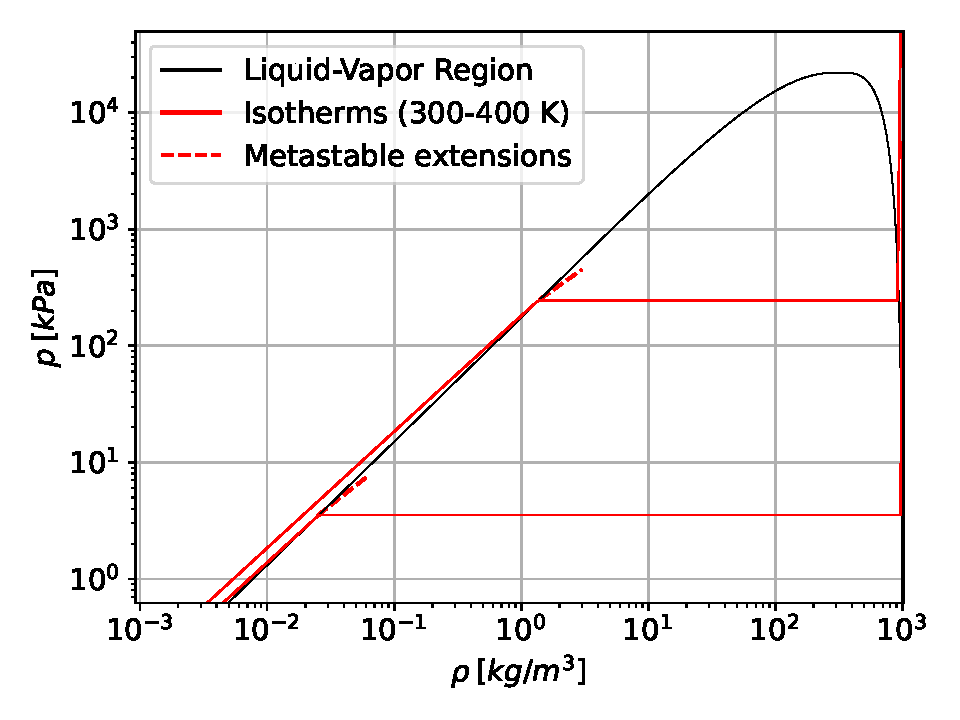
\includegraphics[width=0.7\textwidth]{Figures/metastable_ext.pdf}
    \caption{$p-\rho$ diagram of an isothermally compressed water vapor for two different temperatures. Metastable extensions are conceptually demonstrated as the vapor enters the dome \cite{doi:10.1021/ie4033999}.}
    \label{f:metastable}
\end{figure}
Kalikmanov \cite{kalikmanov2013computer} describes the metastable state as being at a local minimum, with the global minimum being the stable state (condensing). According to Gibbs \cite{gibbs1957method}, a thermodynamic system tends to assume a state of lowest free-energy (the global minimum), however, to get there from the metastable state, the system must overcome a barrier \cite{mcdonald1962homogeneous}. The only way to decrease the free-energy further, the vapor must undergo dropwise condensation, nonetheless, as soon as embryonic droplets form, the surface-free-energy between the liquid and the vapor must be accounted for. Although the bulk-free-energy of the liquid phase provides a reduction of the total free energy, the "unfavored" molecular structure of the interface provides an increase of free-energy to the system. The total free-energy change of the system, $\Delta F$, is formulated by McDonald \cite{mcdonald1962homogeneous}.
\begin{equation}\label{eq:CNT-free_energy}
    \Delta F=4\pi r^{2}\sigma-\frac{4}{3}\pi r^{3}\rho RT \ln\frac{p}{p'}
\end{equation}
Here, $r$ is the radius of the formed droplet, $\sigma$ is the surface tension, $\rho$, $R$, $T$ and $p$ are the density, gas constant, temperature and pressure respectively and $p'$ is the saturation pressure. Due to the quadratic term being larger than the cubic for a very small interval near zero, for very small droplet sizes, the surface term in equation \ref{eq:CNT-free_energy} dominates and further condensation will therefore not occur.
\begin{figure}[h!]
    \centering
    
    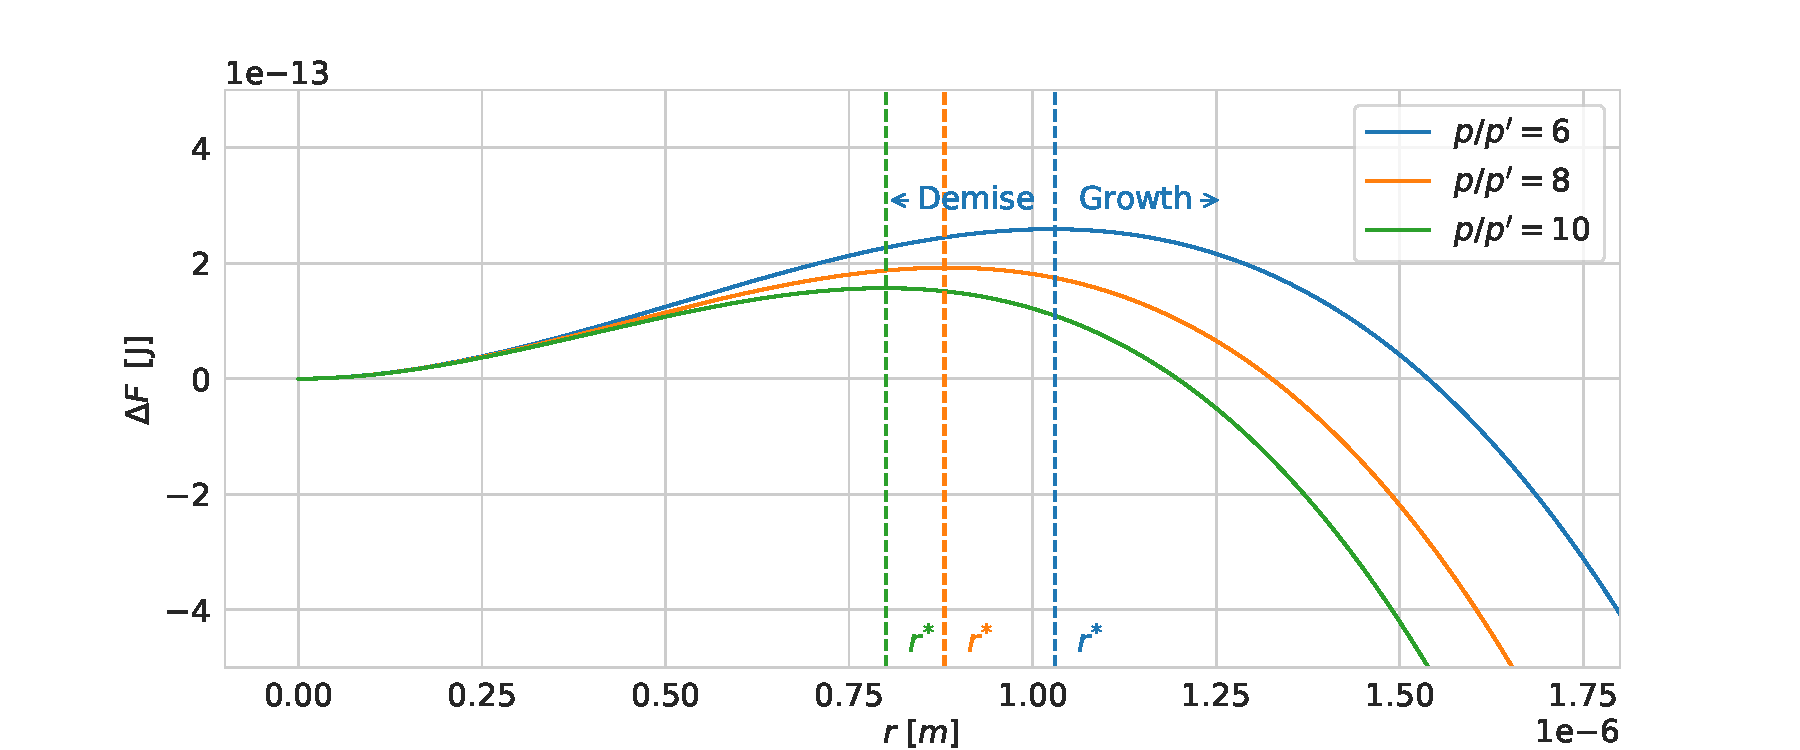
\includegraphics[width=1\textwidth]{Figures/crit_rad_homo.pdf}
    \caption{Gibbs free-energy as a function of the radius for different supersaturation levels. Vertical lines depict the critical droplet radius for each supersaturation level respectively.}
    \label{f:crit_radius for supersat}
\end{figure}
A sub-saturated or just-saturated vapor is however not completely embryo-free. A statistically steady population of embryos exists and can be formulated by a Boltzmann distribution function \cite{mcdonald1962homogeneous}
\begin{equation}\label{eq:CNT stat distribution}
    J_{g}=J_{0}\exp\left[\frac{-\Delta F}{k_{B}T}\right],
\end{equation}
where $J_{g}$ is the number of embryos the size of $g$ (the number of molecules in the embryo) created per second per unit volume of vapor, $J_{0}$ is a pre-exponential constant and $k_{B}$ is the Boltzmann constant. In McDonald's findings, it is shown that at a certain saturation level, larger droplets are significantly less likely to be encountered than smaller ones. However, despite their presence, droplets that nucleate smaller than the critical radius will be unable to overcome the free-energy barrier and will consequently evaporate (see Figure \ref{f:crit_radius for supersat}).
The critical droplet radius, $r^{*}$, dictates the minimum size of nuclei that will impel spontaneous condensation and can be determined by differentiating equation \ref{eq:CNT-free_energy} with respect to the radius \cite{mcdonald1962homogeneous}.
\begin{equation}\label{eq:crit_rad}
    r^{*}=\frac{2\sigma}{\rho RT\ln(p/p')}
\end{equation}
From Eq. \ref{eq:crit_rad} it is clear that in the case of no supersaturation ($p/p'=1$) the critical radius would be infinite and thus there will be only nucleated droplets that will not continue to condense. Moreover, with an increasing degree of supersaturation, the probability will increase that intermolecular fluctuations will send more embryos over the activation barrier and thus more stable droplets will be observed \cite{mcdonald1962homogeneous}. Figure \ref{f:crit_radius for supersat} illustrates the radius that dictates whether freshly nucleated droplets will continue to grow or evaporate again for different supersaturation levels. 

Thus, based on McDonald's article, a conclusion can be drawn that as the supersaturation level increases, the critical radius becomes smaller, leading to statistically more droplets that will pushed over the activation energy barrier. Due to the obvious interest in droplets that will not directly evaporate again, Eq. \ref{eq:crit_rad} can be inserted in Eq. \ref{eq:CNT-free_energy} to acquire the critical energy required. Lastly, inserting the critical work in the Boltzmann distribution will allow to statistically determine the amount of droplets that will form per unit volume of vapor per second, that will remain in an observed domain \cite{mcdonald1962homogeneous}.

% \subsubsection{Diffuse Interface Theory (DIT)}\label{sss:Literature-DIT}
% In contrast to the CNT which assumes a sharp interface, the DIT assumes that the interface between the phases is diffuse \cite{kelton2022theory}. The theory was first published in 1993 and was developed by Gránásy and collaborators \cite{granasy1993diffuse} and was based on good predictions made by the Density Function Theory (DFT), which assumed the diffuse interface. As described by Kelton \cite{kelton2022theory}, Gránásy offered a variation to the DFT proposing a “ready to use” phenomenological thermodynamic approach. 
% The problem with the CNT originates from the capillarity approximation: the assumption that spherical particles possess volume and interface free-energy is only valid if the thickness of the interface is negligible in comparison to the size of the nucleus \cite{granasy1993diffuse}. Gránásy continues and suggests that it is hardly the case for nuclei containing 30 to a few 100 molecules obtained in a lot of cases where the nuclei are almost "all interface" and therefore, a correction to the CNT might be necessary. Furthermore, it is suggested that this conclusion is drawn from the failure of the CNT to predict vapor condensation in various systems \cite{granasy1993diffuse}.

% The key implication of adopting the diffuse interface assumption is that the interface possesses a finite thickness, leading to a dependency of its free-energy on this thickness. To demonstrate this concept, the derivation of the DIT begins with the findings of Turnbull \cite{turnbull1964physics}, which demonstrated that the variation of the physical state of the interface can be characterized by the cross-interfacial enthalpy and entropy distributions. The Gibbs free-energy of formation, $W$, of the new phase is formulated for a symmetric spherical geometry \cite{turnbull1964physics}

% \begin{equation}\label{eq:Turnbull work of formation}
%     \begin{aligned}
%         W&=\int_{0}^{\infty}(\Delta h -T\Delta s)4\pi r^{2}dr\\
%         \Delta h&=\rho_{mol}(r)(H(r)-H_{1})\\
%         \Delta s&=\rho_{mol}(r)(S(r)-S_{1})
%     \end{aligned}
% \end{equation}
% where the specific enthalpy change and entropy change are a function of the local molar density, $\rho_{mol}(r)$ and local molar enthalpy and entropy, where subscript $1$ refers to the parent phase.

% \begin{figure}[h!]
%     \centering
    
%     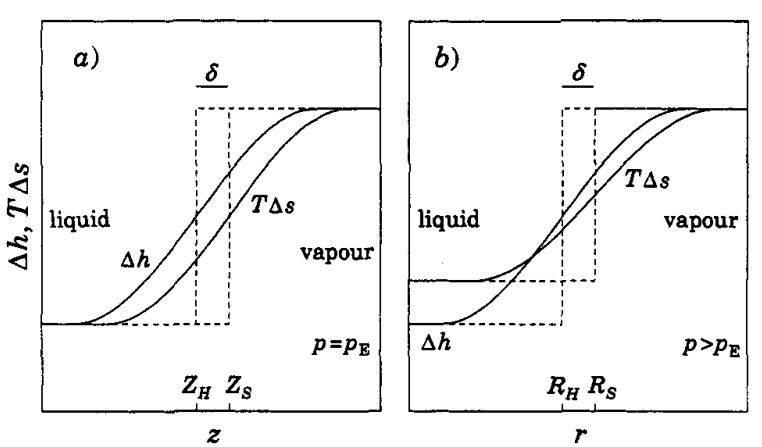
\includegraphics[width=0.7\textwidth]{Figures/Granasy_plot.png}
%     \caption{Conceptualized cross-interfacial enthalpy and entropy of a) planar coordinates and b) radial coordinates. The dotted line represents the step-function approximation \cite{granasy1993diffuse}.}
%     \label{f:cross-interfacial enthalpy and entropy}
% \end{figure}

% Eq. \ref{eq:Turnbull work of formation} can be simplified by approximating the cross-interfacial properties via a step-function (see Figure \ref{f:cross-interfacial enthalpy and entropy}) and thus express $W$ in terms of the enthalpy and entropy surfaces ($R_{H}$ and $R_{S}$ respectively) \cite{granasy1993diffuse}
% \begin{equation}\label{eq:DIT_work of formation}
%     W=\frac{4\pi}{3}(R_{H}^{3}\Delta h_{0}-R_{S}^{3}T\Delta s_{0})
% \end{equation}
% where $\Delta h_{0}$, $\Delta s_{0}$ are the local enthalpy and entropy densities of the droplet at $r=0$, respectively. Hence, the area enclosed between $\Delta h$ and $T\Delta s$  curves is proportional to the interfacial free-energy and the interfacial width is expressed as $\delta =R_{S}-R_{H}$ \cite{kelton2022theory}. Granasy mentions that such simplification may break down for very small embryos, nevertheless, its range of validity may still be larger than that of the CNT \cite{granasy1993diffuse}.

% Similarly to the CNT, by differentiating Eq. \ref{eq:DIT_work of formation} with respect to $R_{S}$, one can find the critical work of formation. 

% \begin{equation}\label{eq: DIT crit work}
%     W^{*}=\frac{(4\pi/3)\delta^{3}\Delta h_{0}T\Delta s_{0}}{\Delta h_{0}+T\Delta s_{0}-2\sqrt{\Delta h_{0}T\Delta s_{0}}}
% \end{equation}
% The critical work of formation $W^{*}$ can then be inserted into Eq. \ref{eq:CNT stat distribution} to acquire the nucleation rate of droplets that overcome $W^{*}$.


% Kelton \cite{kelton2022theory} used the DIT for computer studies of glass nucleation in 2022. Although he acquired good quantitative results with the CNT, he suggests that the theory might break down under conditions far away from equilibrium, hence, the diffuse interface approach might be necessary \cite{kelton2022theory}.
\subsubsection{Droplet Growth in Pure Vapor}\label{sss:Literature-Droplet Growth pure}
After nucleation, the lifespan of the droplets through the simulation domain must be modeled, as it describes the amount of mass that undergoes a phase change and thus contributes to the development of the wetness fraction of the flow \cite{starzmann2010non}. The wetness fraction is the amount of liquid mass per vapor mass. This lifespan is described through a droplet growth model. The vast majority of the considered publications such as \cite{yang2017cfd,zheng2018modeling,liu2020condensation,patel2016influence,gerber2004pressure} model the growth rate after Gyarmathy et al. \cite{gyarmathy1962grundlagen}: Consider an energy balance around a droplet in a pure medium
\begin{equation}\label{eq:knudsen balance}
    h_{vl}\frac{\mathrm{d} m_{l}}{\mathrm{d}t}=4\pi r^{2}h  (T_{l}-T_{v})+m_{l}c_{p,l}\frac{\mathrm{d}T_{l}}{\mathrm{d}t},
\end{equation}
where $m_{l}$, $h_{vl}$, $c_{p,l}$ and $h$ are the droplet's mass, latent heat of evaporation, specific heat and the convective heat transfer coefficient respectively. Subscripts refer to the liquid and vapor phases.
Considering the left-hand side of Eq. \ref{eq:knudsen balance}, the multiplication of the mass change (gain or loss in the case of evaporation) with the latent heat per unit mass is equal to the total latent heat that is removed or added to the droplet. In the case of condensation, a part of the latent heat would be transferred into the droplet through convection and the rest will contribute to changing the temperature of the droplet itself. However, the transient temperature term is neglected as this component is significantly smaller than the convective term for droplets at the size scale considered \cite{gerber2004pressure}. Therefore, Eq. \ref{eq:knudsen balance} can be further simplified and the droplet mass is replaced by the multiplication of the droplet volume with its density ($m_{l}=4/3\pi r^{2}\rho_{l}$)
\begin{equation}\label{eq:knudsen growth rate}
    \frac{\mathrm{d}r}{\mathrm{d}t}=\frac{h(T_{d}-T_{v})}{h_{lv}\rho_{l}}
\end{equation}
Nucleated droplet sizes may or may not be smaller than the average distance traveled by vapor molecules. As a result, the growth of these droplets should be regulated by considering both molecular and macroscopic transport processes, specifically using the Hertz-Knudsen model \cite{wroblewski2009numerical}. However, the application of this model becomes challenging due to the difficulties in selecting the appropriate accommodation coefficient for accurate calculations. This problem will be thoroughly demonstrated and discussed in later sections. To overcome this problem, Gyarmathy's \cite{moore1976two} proposed a model for $h$ which utilizes the Knudsen number. This alternative model incorporates the diffusion of vapor molecules through the surrounding vapor, as well as heat and mass transfer, and factors in the influence of capillarity. $h$ is thus formulated:
\begin{equation}\label{eq:knudsen convection coeff}
    h=\frac{\lambda_{v}}{r(1+3.18\textrm{Kn})}
\end{equation}
\noindent
where $\lambda$ and \textrm{Kn} are the liquid thermal conductivity and the Knudsen number respectively. The Knudsen number is the proportion of the free mean path of vapor molecules and the droplet diameter and is consistently calculated using the formulation of Gyarmathy \cite{gyarmathy1962grundlagen}. The Knudsen number will be further discussed in Section \ref{s:Methodology}. For the sake of simplicity, this droplet growth formulation will be further addressed as the "Knudsen model".

The model offers a simple, ready-to-use formulation of droplet growth and its implementation in a CFD code will be demonstrated in section \ref{sss:Literature-Homogeneous-CFD}. Nevertheless, its limitation is clear: it describes the condensation phenomenon exclusively in a pure vapor domain. Thus, predicting the lifespan of droplets in for example saturated air would not be possible, as field variables such as the mass fraction of vapor in air would not be accounted for. For this, existing evaporation models in such mixtures may be put into use.
\subsubsection{Droplet Evaporation in Mixed Species Domains}\label{sss:Literature-Droplet evaporation}
Under steady and equilibrium conditions, the widely recognized $d^{2}$ evaporation model illustrates the process of evaporation for a solitary suspended droplet within an infinite space \cite{turns2011introduction}. Despite being based on the assumption of an infinite domain, the $d^{2}$-law has been utilized as a benchmark for validating flow solvers that operate within finite computational domains \cite{pathak2018steady}. This can become extremely useful when validating flows within internal combustion engines, as the evaporation process of fuel droplets can be of interest. A thorough derivation of the reversed $d^2$-law (for condensation) will be presented in Section \ref{s:Methodology}, therefore, only the main findings of the evaporation case will be presented here due to their similarity.

Considering a single droplet in an infinite, quiescent gas mixture domain, the derivation of the $d^{2}$ evaporation is presented by Turns \cite{turns2011introduction} and begins with the following assumptions:
\begin{enumerate}
    \item The droplet's evaporation is characterized as quasi-steady, meaning that at any given time, the process can be observed as if it were in a steady state. 
    \item The temperature of the droplet is assumed uniform.
    \item The mass fraction, $Y$ ($\mathrm{kg_{v}/kg_{a}}$), of vapor at the interface is determined by liquid-vapor equilibrium properties.
    \item Thermophysical properties such as mass diffusivity, $\mathcal{D}$, and density, $\rho$, of the mixture remain constant (temperature independent). 
\end{enumerate}
\begin{figure}[h!]
    \centering
    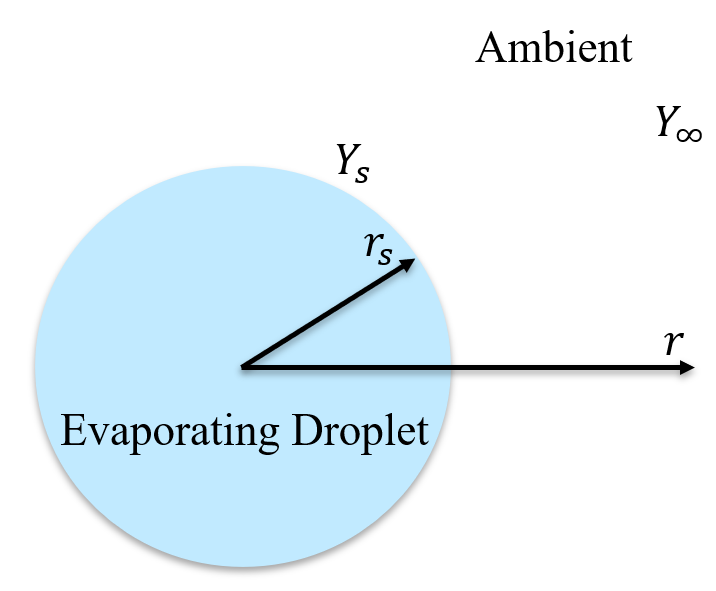
\includegraphics[width=0.4\textwidth]{Figures/Droplet_evap_concept.png}
    \caption{1D Droplet concept in radial coordinates}
    \label{f:D2 concept}
\end{figure}
Figure \ref{f:D2 concept} illustrates the observed domain for the $d^{2}$ derivation. The problem is essentially one-dimensional as the problem is defined in radial coordinates and is independent of any angular coordinates. Furthermore, due to the equilibrium properties assumption at the surface, the mass fraction, $Y_{s}$, can be defined by the saturation value of one species in the other, which can be found using a given temperature and pressure. $Y_{\infty}$, which is the mass fraction infinitely far away from the droplet, must be known or assumed zero in the case of injection of one species into the other \cite{turns2011introduction}. 

The mass conservation of the gas phase is considered
\begin{equation}\label{eq:D2_evap_mass_flux}
    \dot m(r)=\mathrm{constant}=4\pi r^{2}\dot m'',
\end{equation}
where $\dot m''$ is the total mass flux ($\mathrm{kg/m^{2}s}$) and $\dot m''=\dot m''_{A}+\dot m''_{B}=\dot m''_{A}$ (with $A$ and $B$ being, for example, water and air respectively) holds because only one species enters the gas-phase from the droplet. It should be noted, that the mass flow rate is constant and not the mass flux. Then, the species continuity equation is formulated at the droplet interface:
\begin{equation}\label{eq:D2_evap_ficks}
    \rho_{s}v_{s}= \rho_{s}v_{s}Y_{s}-\rho_{s}\mathcal{D}\frac{\mathrm{d}Y}{\mathrm{d}r} 
\end{equation}
Eq. \ref{eq:D2_evap_ficks} can be understood as the total mass flux is equal to the sum of mass flux associated with the bulk flow and mass flux associated with molecular diffusion (Fick's law) \cite{turns2011introduction}. Inserting Eq. \ref{eq:D2_evap_mass_flux} into Eq. \ref{eq:D2_evap_ficks}, rearranging and integrating between the surface value, $Y_{s}$, and at an infinite distance from the droplet, $Y_{\infty}$, yields
\begin{equation}\label{eq:D2_evap_mass_transfer}
    \begin{aligned}
        \dot m&=4\pi r_{s}\rho \mathcal{D}\ln(1+B_{M}),\\
        B_{M}&=\frac{Y_{s}-Y_{\infty}}{1-Y_{s}}    
    \end{aligned}
\end{equation}
$B_{M}$ is referred to as a dimensionless mass transfer number which is interpreted as the "driving potential" for mass transfer, due to the difference in mass fractions \cite{turns2011introduction}. Lastly, by incorporating droplet mass conservation (conservation of the liquid phase),
\begin{equation}
    \frac{\mathrm{d}m_{l}}{\mathrm{d}t}=-\dot m
\end{equation}
reformulating in terms of volume and density and inserting Eq. \ref{eq:D2_evap_mass_transfer} into the right-hand side, the following is acquired:
\begin{equation}\label{eq:D_evap}
    \frac{\mathrm{d}d}{\mathrm{d}t}=-\frac{4\rho\mathcal{D}}{\rho_{l}d}\ln(1+B_{M})
\end{equation}
However, combustion literature usually expresses Eq. \ref{eq:D_evap} in terms of the squared diameter, $d^{2}$, thus 
\begin{equation}\label{eq:D2_evap}
    \frac{\mathrm{d}d^{2}}{\mathrm{d}t}=-\frac{8\rho\mathcal{D}}{\rho_{l}}\ln(1+B_{M})
\end{equation}
According to Eq. \ref{eq:D2_evap}, the time derivatite of $d^{2}$ is constant, which implies that $d^{2}$ changes linearly over time. Labeling the right-hand side of Eq. \ref{eq:D2_evap} (without the sign) as $K$, the $d^{2}$-law is expressed in its common form:
\begin{equation}\label{eq:D2_e}
    d^{2}(t)=-Kt+d_{0}^{2}
\end{equation}
where $d_{0}$ is the initial droplet diameter. Eq. \ref{eq:D2_e} is consistent with experimental data after the newly nucleated droplets undergo an initial transient period \cite{turns2011introduction}. This period can also be observed in the reversed $d^{2}$-law and will be demonstrated in section \ref{s:Results}.

Both droplet growth/evaporation models enable evaluation of the gained/lost mass with respect to time within two different domains and thus influence field variables such as the mass fraction of a given CFD simulation. Nevertheless, Eq. \ref{eq:knudsen growth rate}, most commonly used in condensing turbine simulated flows, will not be solved by iterative means such as 4th order Runge-Kutta (RK45), but rather by averaging of the droplets radii. This is demonstrated in the following section.   
\subsubsection{CFD Models}\label{sss:Literature-Homogeneous-CFD}
The utilization of the aforementioned nucleation and droplet growth models are well demonstrated in research investigating the condensation phenomenon within a steam turbine. Therefore, it should be mentioned that this section will focus mainly on publications concerning this test case. 

When dealing with multi-phase flows, it is essential to select a frame of reference for both phases. Advanced computational fluid dynamics (CFD) codes incorporate an Eulerian/Lagrangian frame of reference, which accurately calculates the trajectories of liquid droplets, leading to precise flow behaviors. Nevertheless, the computational expenses associated with these codes may restrict their accessibility and usage \cite{francesco2017cfd}. This is especially true in turbine flows where nucleation rates can reach up to $10^{23}\:\mathrm{1/m^{3}s}$, hence making droplet tracking very computationally demanding \cite{francesco2017cfd}. As a result, recent studies often suggest an alternative approach that is more computationally accessible: the Eulerian/Eulerian frame of reference, incorporating a volume averaging of the liquid phase equations. However, it is important to note that this reduction in computational expenses comes with the trade-off of lower accuracy \cite{francesco2017cfd}.  Furthermore, the distinction between equilibrium steam models (EQS) and non-equilibrium steam models (NES) also must be made as they affect the formulation of the transport equations: EQS models assume the formation of droplets as soon as the vapor expands into the dome, while NES assumes that the vapor initially remains dry, reaching a non-equilibrium state and its fallback into equilibrium conditions through condensation is associated with an increase of entropy \cite{starzmann2010non}. This process and demonstrated in an enthalpy-entropy ($h-s$) diagram in Figure \ref{f:NES}. The revision to equilibrium conditions ($1_{NE}-1_{EQ^{*}}$) is demonstrated from the extrapolation of the isotherms and isobars into the dome i.e. the metastable extensions (see Figure \ref{f:metastable} for reference). As previously discussed, this revision occurs by droplets that reach the critical radius and allow spontaneous condensation \cite{starzmann2010non}.

Due to EQS models capturing idealized flow conditions \cite{starzmann2010non}, many publications which perform numerical investigations in the Eulerian/Eulerian frame of reference would asses the losses associated with the non-equilibrium conditions. This confirms that the steam turbine test case can serve as a pertinent reference to evaluate the application of the examined nucleation and growth models discussed earlier in the sections.
\begin{figure}[H]
    \centering
    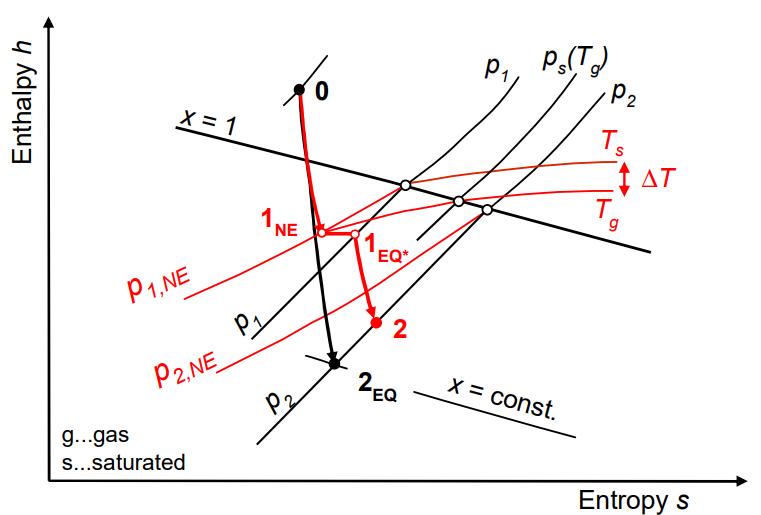
\includegraphics[width=0.7\textwidth]{Figures/NES_h_s.png}
    \caption{Schematic of non-equilibrium expansion within a turbine. Presented by Traupel \cite{traupel1977thermal}.}
    \label{f:NES}
\end{figure}
The conservation equations for this frame of reference and flow conditions are formulated following Gerber and Kermani, and Patel et al. \cite{gerber2004pressure,patel2016influence}:
Mass conservation for the vapor phase, conservation of the droplet number, momentum conservation for the vapor phase and energy conservation for the vapor phase respectively 
\begin{equation}
    \frac{\partial}{\partial t}(\rho_{v}\alpha_{v})+\frac{\partial}{\partial x_{j}}(\rho_{v}\alpha_{v}u_{j,v}) = - S_{d}- m^{*}\alpha_{v}J_{d},  
    \label{eq:v_conti}
\end{equation}
\begin{equation}
     \frac{\partial}{\partial t}(\rho_{l}\eta)+\frac{\partial}{\partial x_{}}(\rho_{l}\eta u_{j,l}) = \rho_{l}\alpha_{v}J_{d},  
    \label{eq:number_conti}
\end{equation}
\begin{equation}
    \frac{\partial}{\partial t}(\rho_{v}\alpha_{v}u_{i,v})+\frac{\partial}{\partial x_{j}}(\rho_{v}\alpha_{v}u_{i,v}u_{j,v}) = -\alpha_{v}\frac{\partial p}{\partial x_{i}}+\frac{\partial}{\partial x_{j}}(\alpha_{v}\tau_{ij,v}) + S_{d}u_{i}, 
    \label{eq:v_momentum}
\end{equation}
 \begin{equation}
    \frac{\partial}{\partial t}(\rho_{v}\alpha_{v}H_{v})+\frac{\partial}{\partial x_{j}}(\rho_{v}\alpha_{v}u_{i,v}H_{v}) =-\alpha_{v}\frac{\partial p}{\partial t}+\frac{\partial}{\partial x_{j}}(\alpha_{v}\Gamma\frac{\partial T_{v}}{\partial x_{j}})+\frac{\partial}{\partial x_{j}}(\alpha_{v}u_{i,v}\tau_{ij,v}) + S_{d}h_{l}, 
    \label{eq:v_energy}
\end{equation}
where $u_{i}$, $H$, $h$, $\Gamma$ and $\tau$ are the velocity component, enthalpy, specific enthalpy of a droplet, thermal diffusion coefficient and viscous stress tensor respectively. $\alpha$ is the volumetric phase fraction ($\alpha=1$ means cell is $100\%$ vapor), $\eta$ is the droplet number per unit volume of vapor ($1/\mathrm{m}^{3}$) and $m^{*}$ is the critical mass of a freshly nucleated droplet. Subscripts remain consistent for the vapor and liquid phases as done previously. Note, that the momentum equation is only formulated for the vapor phase due to negligible drag caused by the droplets. Therefore, it is assumed that both phases possess an identical velocity field \cite{patel2016influence}. This assumption can be otherwise explained by a no-slip condition between the droplets and the vapor. Slip condition could be accounted for by solving an additional transport equation for the liquid phase, however, Wroblewski \cite{wroblewski2009numerical} noted that the no-slip assumption is much less significant than the effects caused by the non-equilibrium conditions. The interaction between the two phases is modeled through the source terms $S_{d}$ and $J_{d}$ which are defined as follows
\begin{equation}
    J_{d}=\frac{1}{1+q_{c}}\sqrt{\frac{2\sigma}{\pi m^{*^{3}}}}\frac{\rho_{v}^{2}}{\rho_{l}}\exp\left[-\frac{4\pi r^{*^{2}}\sigma}{3k_{B}T_{v}}\right],
    \label{eq:nucleation gerber}
\end{equation}
where
\begin{equation}
    q_{c}=2\frac{\gamma-1}{\gamma+1}\frac{h_{vl}}{RT_{v}}\left(\frac{h_{vl}}{RT_{v}}-\frac{1}{2}\right)
    \label{eq:nucleation gerber theta}
\end{equation}
Here, $\gamma$ is the specific heat ratio. $q_{c}$ is a non-isothermal correction factor introduced by Kantrowitz and Arthur \cite{kantrowitz1951nucleation}. The rest of the pre-exponential factor is directly adopted from McDonald \cite{mcdonald1962homogeneous}. Compared to Eq. \ref{eq:CNT stat distribution} it is important to note that only nuclei that overcome that activation barrier (of radius $r^{*}$) are of interest as they will progress through the domain and do not evaporate immediately. $S_{d}$ captures the droplet growth given they will continue to grow through Eq. \ref{eq:nucleation gerber}:
\begin{equation}
    S_{d}=\rho_{v}\frac{3\alpha}{\bar{r}}\frac{\mathrm{d}r}{\mathrm{d}t}
\end{equation}
where the average radius $\bar{r}$ can be derived by considering the average mass of a droplet $\bar{m}$ defined by the droplet number and mass fraction
\begin{equation}\label{eq:average_radius}
    \bar{m}=\frac{\alpha}{\eta}\rho_{v} \rightarrow \bar{r}=\left(\frac{3\alpha\rho_{v}}{4\pi\eta\rho_{l}}\right)^{1/3}   
\end{equation}
and the time derivative of the radius is defined by the Knudsen model (Eq. \ref{eq:knudsen growth rate}) where $\bar{r}$ is inserted to solve the ODE. The temperature of the droplet, used for the calculation of the growth rate can be determined by capillarity effects as a function of the vapor temperature (see \cite{gerber2004pressure}). 

Other aspects of the simulations such as the turbulence models used for Reynolds Averaged Navier-Stokes (RANS) simulations will not be discussed due to the field variables of interest $\eta$ and $\alpha$ not influencing the transport equation directly. However, Patel et. al \cite{patel2016influence} offered a modification to the well-known $SST\:\kappa-\omega$ model by introducing additional source terms in their corresponding transport equations. It was concluded that the nucleation rate and growth rate were significantly influenced due to higher viscous dissipation and thus the temperature distribution was altered \cite{patel2016influence}. Such modifications were not implemented in the current model as it remains inconclusive if they provide more accurate results compared to experimental data.

Lastly, it should be noted that in the considered publications, fluid properties were consistently acquired from the standardized steam tables IAPWS-IF97 (International Association for the Properties of Water and Steam). The considered publications for the homogeneous case are summarized in Table \ref{t:literature-homogeneous}. Publications offering modifications to certain models are underlined and further information is provided in the footnotes.

\begin{table}[H]
\begin{threeparttable}[b]
\centering
% \captionsetup{justification=centering}
\caption{Summary of reviewed work on homogeneous condensation.}
\renewcommand{\arraystretch}{1.2}
\begin{tabular}{||c|c|c|c|c||}
\hline\hline
\textbf{Publication} & \textbf{Nucleation} & \textbf{Droplet Growth} & \textbf{EQS/NES} & \textbf{Turbulence Model}\\ \hline\hline
Bagheri \cite{bagheri2017effects}        &  CNT          &  Other              &  NES       &    Unknown                \\\hline
Brinckman \cite{brinckman2019numerical} \tnote{1}       &   CNT         &   Other             &   NES      &      $\kappa-\epsilon$          \\\hline
Gerber \cite{gerber2004pressure}        &        CNT    &    Knudsen            & NES        &    $\kappa-\epsilon$              \\ \hline
Liu \cite{liu2020condensation}        &   CNT         &      Knudsen          &    Both     &     $\kappa-\epsilon$               \\ \hline
Patel \cite{patel2016influence}        &    CNT        &     Knudsen           &   NES      &   \underline{$SST \:\kappa-\omega$} \tnote{2}             \\\hline
Starzmann \cite{starzmann2010non}        &    CNT       &    Knudsen            &   Both      &   $SST \:\kappa-\omega$               \\\hline
Tabata \cite{tabata2022experimental}        &   CNT         &   \underbar{Knudsen} \tnote{3}             & Both        &     $SST \:\kappa-\omega$               \\\hline
Wroblewski \cite{wroblewski2009numerical}        &    \underbar{CNT} \tnote{4}        &      Knudsen          &  NES       &     $SST \:\kappa-\omega$              \\\hline
\end{tabular}
\begin{tablenotes}
    \item [1] Supercritical $\mathrm{CO_{2}}$ compressor simulated.
    \item [2] Additional source term in transport equation.
    \item [3] Modifications proposed by Young \cite{young1982spontaneous}.
    \item [4] Heterogeneous nucleation due to flow impurities are also modeled.
\end{tablenotes}
\label{t:literature-homogeneous}
\end{threeparttable}
\end{table}
\subsection{Heterogeneous Condensation}\label{ss:Literature-Heterogeneous}
As previously mentioned, heterogeneous condensation implies that the process involves a foreign body such as flow impurities, surfaces etc. When considering cold surfaces, it is now clear that their presence provides the required activation energy to provoke spontaneous phase transformation. Therefore, it is expected that the nucleation process may require a different modeling approach which may be surface-dependent. Moreover, the growth process is also expected to be different, due to the participation of the surface in the heat transfer process.

From a technical standpoint, heterogeneous condensation represents the primary mechanism within a condenser, commonly employed in a closed Rankine cycle. Following expansion in the turbine, the working fluid passes through the condenser, releasing its thermal energy into a colder reservoir until it undergoes a complete phase transformation into liquid form. A schematic of a condenser presented by Massoud \cite{massoud2005engineering} is demonstrated in Figure \ref{f:Condenser_schematic}, where circulating water is used as the cold reservoir.
\begin{figure}[H]
    \centering
    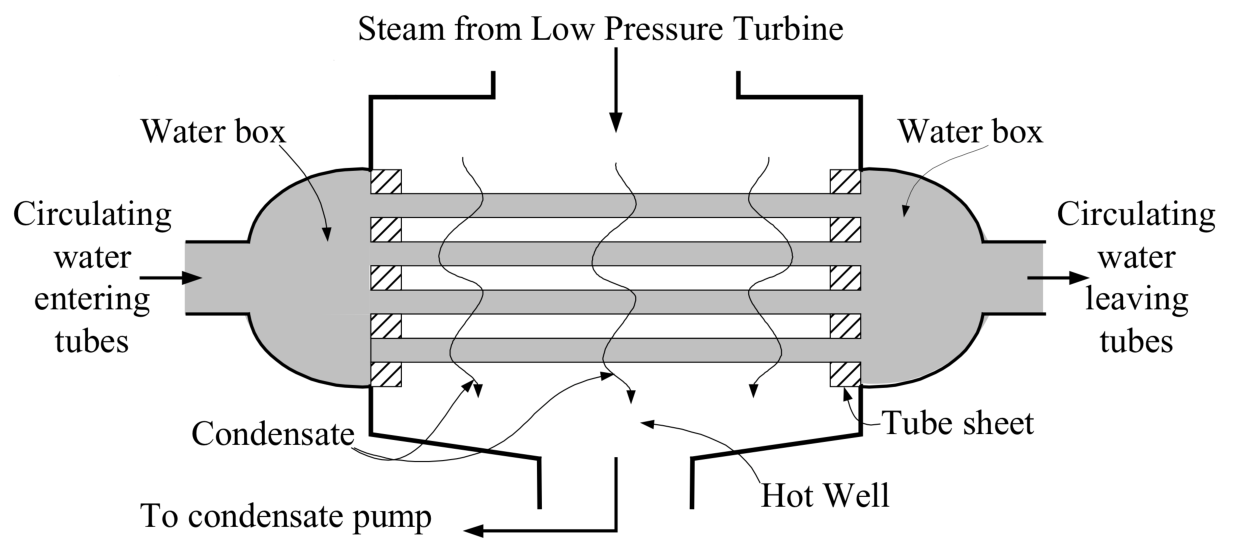
\includegraphics[width=0.8\textwidth]{Figures/Condenser_schematic.pdf}
    \caption{Schematic of a condenser. Presented by Massoud \cite{massoud2005engineering}.}
    \label{f:Condenser_schematic}
\end{figure}
One may observe two types of heterogeneous condensation on the pipes that separate the two fluids \cite{massoud2005engineering}:
\begin{enumerate}
    \item Film condensation occurs when the liquid wets the surface, essentially blanketing it with a liquid film.
    \item Dropwise condensation occurs when the liquid fails to wet the surface, giving rise to discrete droplets that form on the surface instead.
\end{enumerate}
The two scenarios are conceptually demonstrated in Figure \ref{f:drop_vs_film}. Regarding film formation, the substantially larger mass of liquid separating the vapor and the surface leads to reduced heat transfer capabilities. Consequently, under comparable boundary conditions, dropwise condensation exhibits a heat transfer coefficient that can be several magnitudes higher, as reported by Schmidt et al. about 90 years ago \cite{schmidt1930versuche}. Since then, a considerable amount of theoretical and experimental work has been carried out on dropwise condensation \cite{liu2015dropwise}.  
\begin{figure}[H]
    \centering
    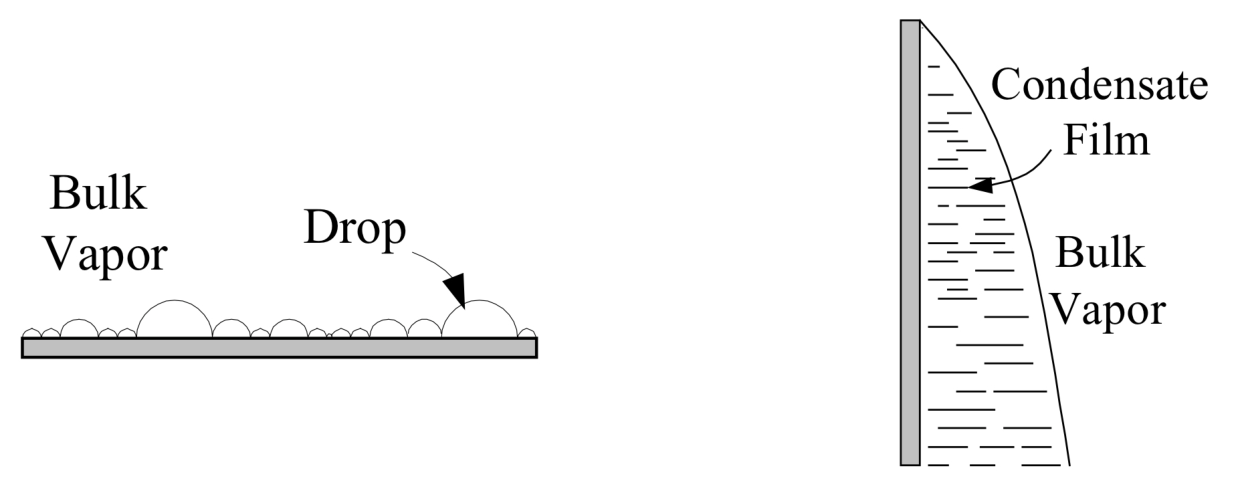
\includegraphics[width=0.8\textwidth]{Figures/Het_Cond_schematic.pdf}
    \caption{Schematic of dropwise condensation (left) and film condensation (right). Presented by Massoud \cite{massoud2005engineering}.}
    \label{f:drop_vs_film}
\end{figure}
However, it should be noted that dropwise condensation has the potential to transition into a film through droplet coalescence (merging of droplets). As a result, this mechanism is of significant interest for further research in understanding the factors that influence it and developing models for CFD applications. The subsequent subsections primarily draw upon the works of Khandekar \cite{khandekar2020drop} and Marengo \cite{marengo2022surface}, as presented in their recent books, which summarize prominent models from previous years. 
\subsubsection{Surface Nucleation}\label{sss:Literature-Heterogeneous-Nucleation}
Macroscopic dropwise condensation occurs as a result of various time-dependent sub-processes involving the creation of drops at nucleation sites, their growth through direct condensation and coalescence, sliding motion and fall-off (in the case of inclined/down-facing substrates), followed by subsequent renucleation on or beneath the substrate. Atomistic modeling of droplet surface formation reveals that the maximal stable cluster formation on an atomic scale is equal to the minimal stable radius derived from thermodynamical principles \cite{khandekar2020drop}. As in the homogeneous case, this critical radius is first sought as it contributes to the calculation of the nucleation site density.

From a chemical potential balance between the two phases at equilibrium conditions, Khandekar reaches a similar critical radius value as seen in Eq. \ref{eq:crit_rad} but in terms of the wall temperature.
\begin{equation}\label{eq:crit_rad_het}
    r_{min}=\frac{2\sigma}{\rho_{v} RT'\ln(p_{v}/p'(T_{w}))}
\end{equation}
Here, subscript $w$ refers to the value of the wall. This time, the critical radius is denoted as $r_{min}$, due to being the smallest possible stable droplet that can nucleate under such conditions \cite{khandekar2020drop}. It is however convenient to acquire $r_{min}$ in terms of the wall and vapor temperatures as they offer more direct boundary conditions. By combining the Clapeyron equation  with the ideal gas law and integrating between $p_{v}$ and $p'$ the following is acquired:
\begin{equation}
    \begin{aligned}
        \frac{\mathrm{d}p}{\mathrm{d}T}&=\frac{ph_{lv}}{RT_{w}^{2}} \\
        \int_{p'}^{p_{v}}\frac{\mathrm{d}p}{p}&=\frac{h_{lv}}{RT_{w}^{2}} \int_{T_{w}}^{T'}\mathrm{d}T\\
        \rightarrow\ln(p_{v}/p'(T_{w}))&=\frac{h_{lv}}{RT_{w}^{2}}(T'-T_{w})       
    \end{aligned}\label{eq:clapeyron_ideal_integration}
\end{equation}
Substituting Eq. \ref{eq:clapeyron_ideal_integration} into Eq. \ref{eq:crit_rad_het} the minimal radius in terms of temperatures is acquired:
\begin{equation}\label{eq:r_min_temp}
    r_{min}=\frac{2\sigma T'}{\rho_{v} h_{lv}(T'-T_{w})}
\end{equation}

In most applications, the magnitude of $r_{min}$ is typically a few nanometers. As a result, capturing the initial nucleation phenomenon on a surface exposed to vapor is challenging experimentally \cite{khandekar2020drop}. Additionally, the nucleation site density is influenced by various factors such as the thermophysical properties of the fluid, physio-chemical properties of the surface, and surface morphology. Consequently, determining the nucleation site density from either theoretical approaches or experiments is also a difficult task \cite{khandekar2020drop}. An empirical expression that yields an estimation of the nucleation site density, $N_{s}$, was proposed by Rose \cite{rose1976further} in 1976 for an untreated surface
\begin{equation}\label{eq:nucleation_site_density}
    N_{s}=\frac{0.037}{r_{min}^{2}}
\end{equation}
In affirmation of this statement, Zhao and Beysens \cite{zhao1995droplet} conducted experiments and found no notable association between the nucleation site density and the wettability of the condensing fluid. Nevertheless, it is essential to note that wettability does have a substantial impact on the droplet growth process, as discussed and demonstrated in the forthcoming section \cite{khandekar2020drop}. Marengo \cite{marengo2022surface} and Liu and Cheng \cite{liu2015dropwise} argued however that the nucleation site density calculated through Eq. \ref{eq:nucleation_site_density} tends to massively overestimate the real value for most applications. Therefore, in this study, $N_{s}$ will be consistently fixed to values reported by other works to match simulated conditions.

\subsubsection{Droplet Growth}\label{sss:Literature-Heterogeneous-Growth}
Unlike the homogeneous scenario, droplets in contact with a substrate experience mass gain solely through their free surface, which is the part of the droplet exposed to the vapor phase. The extent of this surface growth directly depends on the droplet's wettability. Wettability can be understood as the affinity of the liquid to the solid surface \cite{khandekar2020drop}. The shape and behavior of liquids on a solid surface depend on the surface energy of the solid-liquid interface. Liquids with low affinity for the solid will tend to gather into nearly spherical droplets, while liquids with high affinity for the solid will spread out to form a thin film, maximizing the contact area between the liquid and the solid surface \cite{khandekar2020drop}. Wettability can be quantified through the contact angle, $\theta$, and is portrayed in Figure \ref{f: dropwise growth}. $\theta$ can be derived through a force balance between the interfacial tensions, however, it does not pose great significance to the study at hand and therefore will not be demonstrated. Nevertheless, the contact angle provides information about the interactions occurring at different interfaces, encompassing solid/liquid, liquid/gas, solid/gas, and solid/liquid/gas interfaces. The surface tension between phases and further influence from surface roughness can be found in the literature \cite{doble2007perry,khandekar2020drop} or from empirical data. 
\begin{figure}[H]
    \centering
    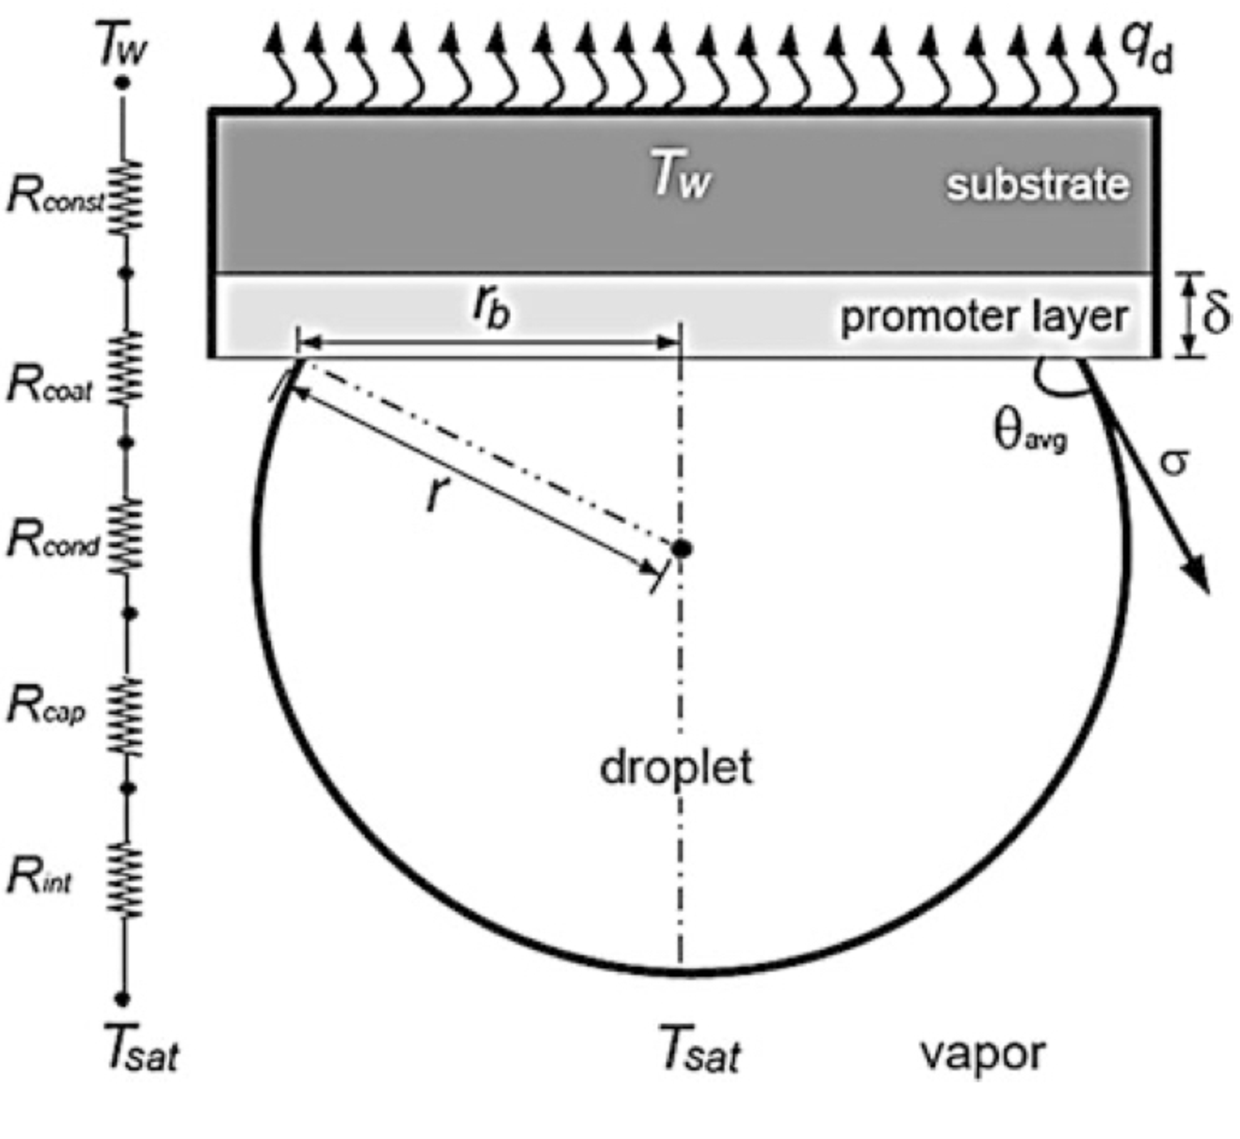
\includegraphics[width=0.5\textwidth]{Figures/Dropwise_growth.pdf}
    \caption{Schematic of thermal resistances for droplet growth. Presented by Khandekar \cite{khandekar2020drop}.}
    \label{f: dropwise growth}
\end{figure}
\noindent
The following angle ranges are classified:
\begin{itemize}
    \item Hydrophilic: wetting ($0^\circ<\theta<90^\circ$)
    \item Hydrophobic: partial wetting ($90^\circ<\theta<140^\circ$)
    \item Superhydrophobic: non-wetting ($140^\circ<\theta<180^\circ$)
\end{itemize}
Other than determining the size of the mass exchange surface between the vapor and the liquid, the contact angle also dictates the size of the surface between the liquid and the solid, thus, having implications on the amount of thermal energy transferred into the solid.

The latent heat release between the vapor-liquid interface is transferred through the volume of the droplet into the substrate. The proposed growth model is based on various thermal resistances in the path of heat transfer. These resistances are conceptually demonstrated in Figure \ref{f: dropwise growth} and are listed as follows \cite{khandekar2020drop}:
\begin{enumerate}
    \item Vapor-liquid interface resistance ($R_{int}$)
    \item Capillary resistance ($R_{cap}$) refers to the reduction in the driving temperature potential caused by the curvature of the interface
    \item Resistance due to heat conduction ($R_{cond}$) through the droplet 
    \item Constriction resistance ($R_{const}$) associated with substrate thermal conductivity 
\end{enumerate}
The promoter layer resistance seen in Figure \ref{f: dropwise growth} is not considered in this work.
The total temperature difference between the saturated vapor and the solid substrate is equal to the sum of temperature drops due to the resistances.
\begin{equation}
    T'-T_w=\Delta T_{cond}+\Delta T_{int}+\Delta T_{cap}+\Delta T_{const}
\end{equation}
In Appendix \ref{s:appendix A}, each temperature difference is thoroughly described and expressed in relation to the total heat transferred to the substrate. By employing the relationship that equates the total heat transferred through a droplet of a specific radius to the product of the mass flow rate and the latent heat, it becomes possible to represent the time derivative of the radius \cite{khandekar2020drop}. 
\begin{equation}\label{eq:het_droplet_growth}
        \frac{\mathrm{d}r}{\mathrm{d}t}= \left(\frac{4(T'-T_{w})}{\rho_{l}h_{vl}}\right)(1-\frac{r_{min}}{r})\left(\frac{2}{h_{int}}+\frac{r(1-\cos\theta)}{\lambda_{l}}\right)^{-1}  \cdot\left(\frac{1-\cos\theta}{2-3\cos\theta+\cos^{3}\theta}\right)
\end{equation}
where $\lambda_{l}$ and $h_{int}$ are the thermal conductivity of the droplet and the interfacial heat transfer coefficient respectively. $r_{min}$ is defined by Eq. \ref{eq:crit_rad_het}. Eq. \ref{eq:het_droplet_growth} is valid for either horizontal or inclined surfaces without a wettability gradient. Note that the thermal conductivity of the substrate does not appear in Eq. \ref{eq:het_droplet_growth}. The significance of the thermal conductivity of the condensing surface in the condensation process has been a subject of controversy. In situations where the assumption of uniform substrate temperature is made, no additional terms are taken into account, as pointed out by Khandekar \cite{khandekar2020drop}. However, this assumption may not hold true when considering a condenser configuration depicted in Figure \ref{f:Condenser_schematic}. Depending on the boundary conditions, it becomes essential to assess whether the pipe walls can be categorized as thermally "thin" or "thick" (by evaluating the Biot number) to determine the presence of a significant temperature gradient across them. 
%  For an inclined case, it is important to note that an average contact angle would be used for simplicity \cite{khandekar2020drop}.

Depending on the conditions of interest, growth by coalescence can occur when neighboring droplets come into contact when reaching sufficient size. For inclined substrate cases, coalescence can also occur when droplets reach a size that would satisfy a slide-off criteria (force of gravity would overcome the surface tension), thus merging with droplets in their path. Such phenomena add a significant amount of complexity to a CFD model and will not be directly considered in this work. However, it will be shown that the intricacies of this mechanism do not necessarily need to be modeled to acquire good estimations of variables such as the wall heat flux for a given droplet distribution. 
\subsubsection{Droplet Population Density and Wall Heat Flux}
Marengo \cite{marengo2022surface} describes dropwise condensation as a cyclic process that follows the following steps:
\begin{enumerate}
    \item Droplets of radius $r_{min}$ (determined thermodynamically, Eq. \ref{eq:r_min_temp}) form on favored nucleation sites, determined by substrate temperature, surface impurities etc.
    \item The droplets grow by direct condensation at first, possibly later by coalescence, until they reach a departing radius $r_{max}$, at which body forces overcome the surface adhesion and the droplets sweep away.
    \item Once swept, new surfaces are exposed for renewed nucleation.
\end{enumerate} 
Given this repetitive pattern, a nucleation site can manage droplets of diverse sizes spanning various length scales and undergo processes that vary over different time scales. Additionally, dealing with droplets at the smallest length scales remains challenging from an experimental perspective, as measurement techniques continue to pose difficulties to this day. The implementation of accurate CFD models for dropwise condensation is therefore of limited feasibility \cite{marengo2022surface}. Nevertheless, droplet population models also known as droplet size distribution models attempt to capture this cyclic behavior. They rely on the premise that the drop size distribution on a condensing surface remains in a statistically stable state \cite{marengo2022surface}.

The model proposed by Le Fevre and Rose in 1966 \cite{le1966theory} is often referenced in recent literature. This empirical expression describes the droplet population, $N(r)$, for droplets ranging from $r_{min}-r_{max}$.
\begin{equation}\label{eq:droplet_population}
    N(r)=\frac{1}{3\pi r^{2}r_{max}}\left(\frac{r}{r_{max}}\right)^{-2/3}
\end{equation}
From Eq. \ref{eq:droplet_population} it can be observed that the droplet size population only depends on the maximal radius, $r_{max}$, which is derived through the forces acting on the droplets. It's important to note that newer models enhance and refine this representation by integrating supplementary population models for smaller droplets and by accounting for various time scales within the condensation process \cite{marengo2022surface}. The difference in results will be presented in Section \ref{s:Results}. Nevertheless, these newer models add significant complexity which proves to be difficult to incorporate in an Eulerian/Eulerian code. Thus, the model proposed by Le Fevre and Rose will be used in this work.

If assumed that the vapor temperature is uniform and equal to saturation conditions, quiescent domain and no presence of non-condensable gases, by integrating the product of $N(r)$ with the heat transfer through a single droplet, $Q_{d}$, the average heat flux to the wall, $q$, can be obtained \cite{marengo2022surface}.
\begin{equation}\label{eq:wall_heat_flux}
    q=\int_{r_{min}}^{r_{max}}Q_{d}(r)N(r)\mathrm{d}r 
\end{equation} 
$Q_{d}$ can be obtained by knowledge of the radius rate of change (Eq. \ref{eq:het_droplet_growth}). This expression holds significant value as it enables the potential for comparing simulation outcomes to experimental data, primarily because $q$ is a quantifiable parameter. Eq. \ref{eq:wall_heat_flux} can be explained with words rather intuitively: the wall heat flux is represented by the life cycle of all droplets of different sizes multiplied by their respective heat transfer.
\subsubsection{CFD Models}\label{sss:Literature-Heterogeneous-CFD}
The majority of found literature employs the volume of fluid interface tracking methods (VOF) to simulate heterogeneous condensation. Such models may deliver accurate depictions of single droplet dynamics. Nevertheless, it is clear that when considering a nucleation site density of $10^{12}$ droplets, surface tracking will not be feasible. A question may be raised if specific droplet dynamics need to be accurately modeled altogether. Eulerian/Eulerian methods may be able to answer this question

The formulation of the transport equations used for an Eulerian/Eulerian frame of reference remains similar to that of the homogeneous case (Eqs. \ref{eq:v_conti}-\ref{eq:v_energy}) as presented by Janet et al. \cite{janet2015heterogeneous} who studied heterogeneous bubble nucleation in a converging-diverging nozzle. The changes employed occur evidently in the respective source terms. Note that Janet's work models heterogeneous condensation in a highly convective flow, which is not the case in a condenser. Nevertheless, principles from this publication can be utilized effectively.

At first, the area-based nucleation rate $S_{nu,A}$ is defined for a given domain in the following manner \cite{janet2015heterogeneous}
\begin{equation}
    S_{nu,A}=\begin{cases}
      J_{het}A & \text{for $A\subset \partial\Omega$}.\\
      0 & \text{otherwise}
    \end{cases}
\end{equation}
where $A$ is the surface area and $\partial\Omega$ is the wall boundary patch. Given a nucleation site density, $N_{s}$, it is possible to formulate a volumetric flux of droplets, $S_{nu}$, on the wall-adjacent cell by accessing the geometric properties of the mesh \cite{janet2015heterogeneous}.
\begin{equation}
    \begin{aligned}
        S_{nu}&=J_{het}\frac{A_{cell}}{V_{cell}}\\
        J_{het}&=fN_{s}
    \end{aligned}
\end{equation} 
Here, $A_{cell}$ and $V_{cell}$ represent the surface area of the cell face adjacent to the wall and the volume of that cell respectively. $f$ represents the nucleation frequency. $f$ may pose difficulties if considering a quiescent domain or not inclined substrates. This is due to the inability of the droplets to be transported away from the wall and thus not allowing exposure of surfaces for renewed nucleation. This will be addressed in Section \ref{s:Methodology}.

In his work, Wroblewski \cite{wroblewski2009numerical} conducted a thorough investigation into both homogeneous and heterogeneous condensation occurring within a steam turbine, employing both numerical simulations and experimental analysis. The study revealed that in heavily contaminated steam, heterogeneous condensation plays a more significant role in contributing to the wetness fraction. This conclusion was substantiated by comparing the results with experimental data. For the droplet growth source term, the formulation was similar to the homogeneous case, where the droplet growth ordinary differential equation (ODE) was solved using the average radius derived from the droplet number and phase volumetric fraction (Eq. \ref{eq:average_radius}).
\subsection{Discussion}\label{ss:Literature-discussion}
Due to dropwise condensation being a highly attractive topic in the past century, there exists a very large variety of models attempting to describe this process. This work was based on more recent literature, which presents models that have been acquired through many years of trial and error. The reasoning behind failed models could have provided better insight into the droplet growth rate and droplet population models, which could potentially assist in finding critical components in the proposed Eulerian/Eulerian model. If the proposed model is to be improved for future work, further literature would be needed to identify potential enhancements.

As part of the research project focused on the reversion of the $d^{2}$ evaporation law, no further models for air-vapor mixture condensation were inspected. Therefore, no quantitative comparisons to the literature were performed. Additional literature demonstrating other models would be useful to acquire further insight on air-vapor mixtures and further adjustment of the derived model could have been performed.

The review for the homogeneous scenario consisted of literature focusing on the steam turbine case. Although this case may provide a good basis for understanding the physical phenomenon, it includes correction terms and modifications to models which may be applicable in compressible transonic flows, but not applicable in other scenarios. The objective of this research project does not consist of understanding the complexities of such flows but rather purely of the condensation phenomenon. Thus it must be addressed that further literature in other flow configurations may have assisted in identifying such modifications, and perhaps provide insight into changes needed for the simulated cylinder case. Moreover, other droplet growth models may have been identified. Nevertheless, the principles of an Eulerian/Eulerian code were well demonstrated and assisted in constructing such code for the heterogeneous case. 


\newpage
\section{Methodology}\label{s:Methodology}
The considered models presented in Section \ref{s:Literature} were utilized and manipulated to provide solutions to various flow configurations. In this section, the solution procedure to these models will be presented and discussed. The following cases are to be investigated
\begin{enumerate}
    \item An extensive comparative and parametric analysis was carried out for droplet growth models. The Knudsen model, as proposed by Gyarmathy \cite{gyarmathy1962grundlagen}, the surface dropwise model presented by Khandekar \cite{khandekar2020drop}, and the derived $d^{2}$ condensation model were solved iteratively in Python and are presented in the form of a Pseudocode (Section \ref{ss:Methodology-Droplet Growth}).
    \item Cylinder case: A solver describing homogeneous nucleation and droplet growth following the CNT and Knudsen model respectively was implemented in OpenFOAM. Steady RANS simulations were conducted for different inlet conditions (Section \ref{ss:Methodology-Homogeneous}).
    \item Flat plate case: a solver describing heterogeneous nucleation and droplet growth on a cooled plate based on the work of Khandekar and Marengo \cite{khandekar2020drop,marengo2022surface} was implemented in OpenFOAM. Unsteady simulations were conducted and heat flux values were compared to values from the literature (Section \ref{ss:Methodology-Heterogeneous}).
\end{enumerate} 
 
\subsection{Droplet Growth}\label{ss:Methodology-Droplet Growth}
\subsubsection{Homogeneous Condensation in Pure Vapor}\label{sss:Methodology-Droplet-pure}
The Knudsen model (Eq. \ref{eq:knudsen growth rate}) is a first-order ODE. As seen in Section \ref{s:Literature}, CFD methods in the Eulerian/Eulerian frame of reference use the mean radius calculated from field variables to estimate the average time derivative of the radius. When investigating a single droplet, the equation can be treated as an initial value problem: given an initial radius, its progression in time can be solved using iterative methods. The explicit 4th-order Runge-Kutte (RK45) method was used to solve Eq. \ref{eq:knudsen growth rate}. For this, the Knudsen number, \textrm{Kn}, is first defined from the kinematics of gas dynamics \cite{gyarmathy1962grundlagen}
\begin{equation}
    \textrm{Kn}=\frac{(1.5\mu_{v}\sqrt{RT_{v}})/p}{2r}
\end{equation}   
as the proportion of the mean free path and the physical length scale (droplet diameter in this case). $\mu_{v}$ is the dynamic viscosity of the vapor. The mean free path refers to the average path that a water molecule travels before colliding with other molecules \cite{gyarmathy1962grundlagen}. Specifically, the continuum assumption remains valid only when the Knudsen number is smaller than $\textrm{Kn}<0.01$. A small \textrm{Kn} value implies that the droplet size is significantly larger than the mean free path of molecules, and as a result, specific molecular trajectories that could interact with the droplet need not be considered. Nevertheless, for very high supersaturation levels and thus the formation of extremely small nuclei is possible, $\mathrm{Kn}$ may be larger than this value. Its multiplication with the empirical constant and the droplet radius (see Eq. \ref{eq:knudsen convection coeff}) offers a correction to the droplet growth rate.

A demonstration of the code written in Python is expressed in Algorithm \ref{alg:knudsen} in the form of a Pseudocode.

\begin{algorithm}
    \caption{Knudsen Droplet Growth Model}
    \label{alg:knudsen}
    \begin{algorithmic}[1]
    \State \textbf{Initialize}: Boundary Conditions: $T_{l}$, $T_{\infty}$, $r_{0}$ \Comment{$r_{0}$: initial droplet size}
    \State \textbf{Initialize}: $\mathrm{d}t$ \Comment{time step of evaluated points}
    \State \textbf{Compute}: $p$ at $T_{\infty}$ \\  
    \quad \quad \quad \quad \quad$\lambda_{v}$ at $T_{\infty}$ \\
    \quad \quad \quad \quad \quad $h_{vl}$ at $p$\\
    \quad \quad \quad \quad \quad$\mu_{v}$ at $T_{\infty}$\\
    \quad \quad \quad \quad \quad $\rho_{l}$ at $T_{l}$ \\
    \quad \quad \quad \quad \quad $l=(1.5\mu_{v}\sqrt{T_{\infty}R})/p$ \Comment{Charactaristic length scale}\\ 
    \quad \quad \quad \quad \quad $\textrm{Kn}=l/2r_{0}$
    
    \State \textbf{Solve}: $\frac{\mathrm{d}r}{\mathrm{d}t}=\frac{\lambda_{v}}{r(1+3.18\textrm{Kn})}\frac{T_{l}-T_{\infty}}{h_{vl}\rho_{l}}$ \Comment{Eq. \ref{eq:knudsen growth rate} solved using RK45 method}
    \end{algorithmic}
\end{algorithm}
It should be noted that thermophysical and transport properties are calculated using various fitting functions based on empirical data proposed by Doble \cite{doble2007perry}. These can be found in Table \ref{t:perry_calcs} in Appendix \ref{s:appendix B}.

Lastly, due to the pure vapor assumption, $p$ must be determined by the temperature as the existence of pure vapor cannot be assumed under any given conditions. Therefore, it is calculated using the definition of the critical radius (Eq. \ref{eq:crit_rad}), thus imposing supersaturated conditions. 

\subsubsection{Homogeneous Condensation in Gas Mixtures}\label{sss:Methodology-Droplet-mix}
Because the Knudsen model is constrained in representing the growth of a condensing droplet in atmospheric conditions, involving a mixture of vapor and air, the $d^{2}$ evaporation model was modified to facilitate the simulation of the reversed process, namely condensation.

Firstly, quasi-steadiness of the droplet growth process can be demonstrated in the following manner. Consider the rate of the droplets mass change is equal to the mass entering the droplet
\begin{equation}
    \frac{\mathrm{d}}{\mathrm{d}t}(4/3 \pi r_{s}^{3}\rho_{l})=\dot {m},
\end{equation}
with the liquid density, $\rho_{l}$, assumed constant. Expanding the right-hand side to be equal to the mass flow rate from the gas phase, the following can be written
\begin{equation}
    \begin{aligned}
        4/3\pi \rho_{l}r_{s}^{2}\frac{\mathrm{d}r_{s}}{\mathrm{d}t}&=4\pi r_{s}^{2}\rho_{g}v \\
        \rightarrow \frac{\mathrm{d}r_{s}}{\mathrm{d}t}&=\frac{\rho_{g}}{\rho_{l}}v,
    \end{aligned}
\end{equation}
with $v$ being the velocity of the vapor due to diffusion. Because the proportion of densities is significantly smaller than 1, it can be concluded that the time derivative of the radius is much smaller than the velocity of the vapor due to mass diffusion. In other words, observing the droplet from the gas phase would seem as if the droplet does not change in size due to the significant difference in speed of the two processes. A time-scale analysis however is beyond the scope of this work and will not be demonstrated. 

The species conservation equation for the gas phase is formulated in its general form without a transient term due to the aforementioned assumption
\begin{equation}\label{eq: D2 species conservation}
     \frac{\partial }{\partial r}(r^{2}\rho_{g} vY)=\frac{\partial}{\partial r}\left (r^{2}\mathcal{D} \rho_{g} \frac{\partial Y}{\partial r} \right )
\end{equation}
Eq. \ref{eq: D2 species conservation} can be integrated over both sides of the droplet's interface and employing boundary conditions
\begin{equation}
     \left[(r^{2}\rho_{g} vY)-\left(r^{2} \rho_{g} \mathcal{D} \frac{\partial Y}{\partial r}\right)\right]_{s+}^{s-} =0
\end{equation}
where $s-$ and $s+$ are at positions within and outside the droplet respectively. Two boundaries are known within the droplet regarding the mass fraction: a) the droplet only consists of the water phase, thus, $Y|_{s-}=1$. b) There exists no concentration gradient of water within the droplet, thus, $\frac{\partial Y}{\partial r}|_{s-}=0$. The following balance is acquired:
\begin{equation}\label{eq:D2_cond_ficks}
    \rho_{g} v= \rho_{g} vY-\rho_{g}\mathcal{D}\frac{\mathrm{d}Y}{\mathrm{d}r} 
\end{equation}
Eq. \ref{eq:D2_cond_ficks} can be understood as the total mass flux is equal to the sum of mass flux associated with the bulk flow and mass flux associated with molecular diffusion (Fick's law) \cite{turns2011introduction}. When observing the gas phase mass conservation, the droplet can be considered a sink. Because $\rho_{g} v$ is nothing else than the mass flux, a negative mass flow rate divided by the surface area of the droplet is inserted into Eq. \ref{eq:D2_cond_ficks}. Then, the Fourier method is used to integrate across the domain between the droplet surface and an infinite distance away from it  
\begin{equation}\label{eq:D2 _mass_transfer_concen}
    \begin{aligned}
        (Y-1)\frac{\dot m}{4\pi r^{2}}&=-\rho_{g} \mathcal{D}\frac{\mathrm{d}Y}{\mathrm{d}r}\\
        \rightarrow \dot m&=-4\pi \rho_{g}r_{s}\mathcal{D}\ln\left({\frac{Y_{\infty}-1}{Y_{s}-1}}\right)
    \end{aligned}
\end{equation}
Similarly to the evaporation case, the term in the natural logarithmic function can be put in the following form
\begin{equation}
    \frac{Y_{\infty}-1}{Y_{s}-1}=1+B_{M}\Longleftrightarrow B_{M}=\frac{Y_{\infty}-Y_{s}}{Y_{s}-1}
\end{equation}
In this form, it becomes clear that the mass fraction at the droplet surface may not surpass that far away from the droplet due to the nature of a logarithmic function. Otherwise, the term in the logarithmic function ($1+B_{M}$) will be larger than one and the mass flow rate will be negative (evaporation). However, it is taken that the mass fraction reaches a saturation value at the surface. This assumption arises from the demonstrated quasi-steadiness of the process, indicating that the vapor transport is much faster than the mass growth process. It can be shown that $Y_{s}'$ can be calculated as follows \cite{turns2011introduction}
\begin{equation}
    Y_{s}'=\frac{p'W_{w}}{p'W_{w}+(p-p')W_{a}}
\end{equation}
where $W$ is the molecular weight of water or air and $p'$ can be calculated using the Clasius-Clapeyron equation. It remains therefore to determine the value of $Y_{\infty}$. If latent heat is to be extracted out of the droplet and hence provoke further mass gain, as for the Knudsen model, the temperature of the droplet must be higher than that of the vapor phase. However, higher temperatures indicate higher saturation pressure, thus indicating that the ambient must be supersaturated. This finding is consistent with the classical nucleation theory: droplets will only continue to condense after nucleation in the case that they reach a critical radius, which is only available in supersaturated conditions. Thus, it is proposed that $Y_{\infty}$ is calculated using the Kelvin equation. A simple derivation from hydrostatic principles was demonstrated by Galvin \cite{GALVIN20054659} where it was shown that the pressure exerted from a fluid on a curved surface is higher than that on a flat plate. In terms of mass concentration:
\begin{equation}\label{eq:kelvin}
    Y_{\infty}=Y_{s}'(T_{s})\exp\left(\frac{2W_{w}\sigma}{N_{A}k_{B}T_{s}\rho_{l}r_{s}}\right)
\end{equation}
Reformulating Eq. \ref{eq:kelvin} in terms of $r_{s}$ would yield a very similar expression to the critical radius derived by Gibbs. The Kelvin equation can be considered as imposing the CNT on the $d^2$ condensation model, or in other words, given an initial droplet radius, what supersaturation level is required to achieve growth. 

Figure \ref{f:kelvin_supersat} illustrates the required supersaturation level for continued droplet condensation. For example, Gerber et al. \cite{gerber2004pressure} observed droplet nucleation sizes in this scenario ranging between $10^{-9}<r_{s}<10^{-7}$. Although he considered pure vapor, it is still evident that smaller droplets may necessitate a substantial supersaturation level, while larger droplets require minimal supersaturation.
\begin{figure}[H]
    \centering
    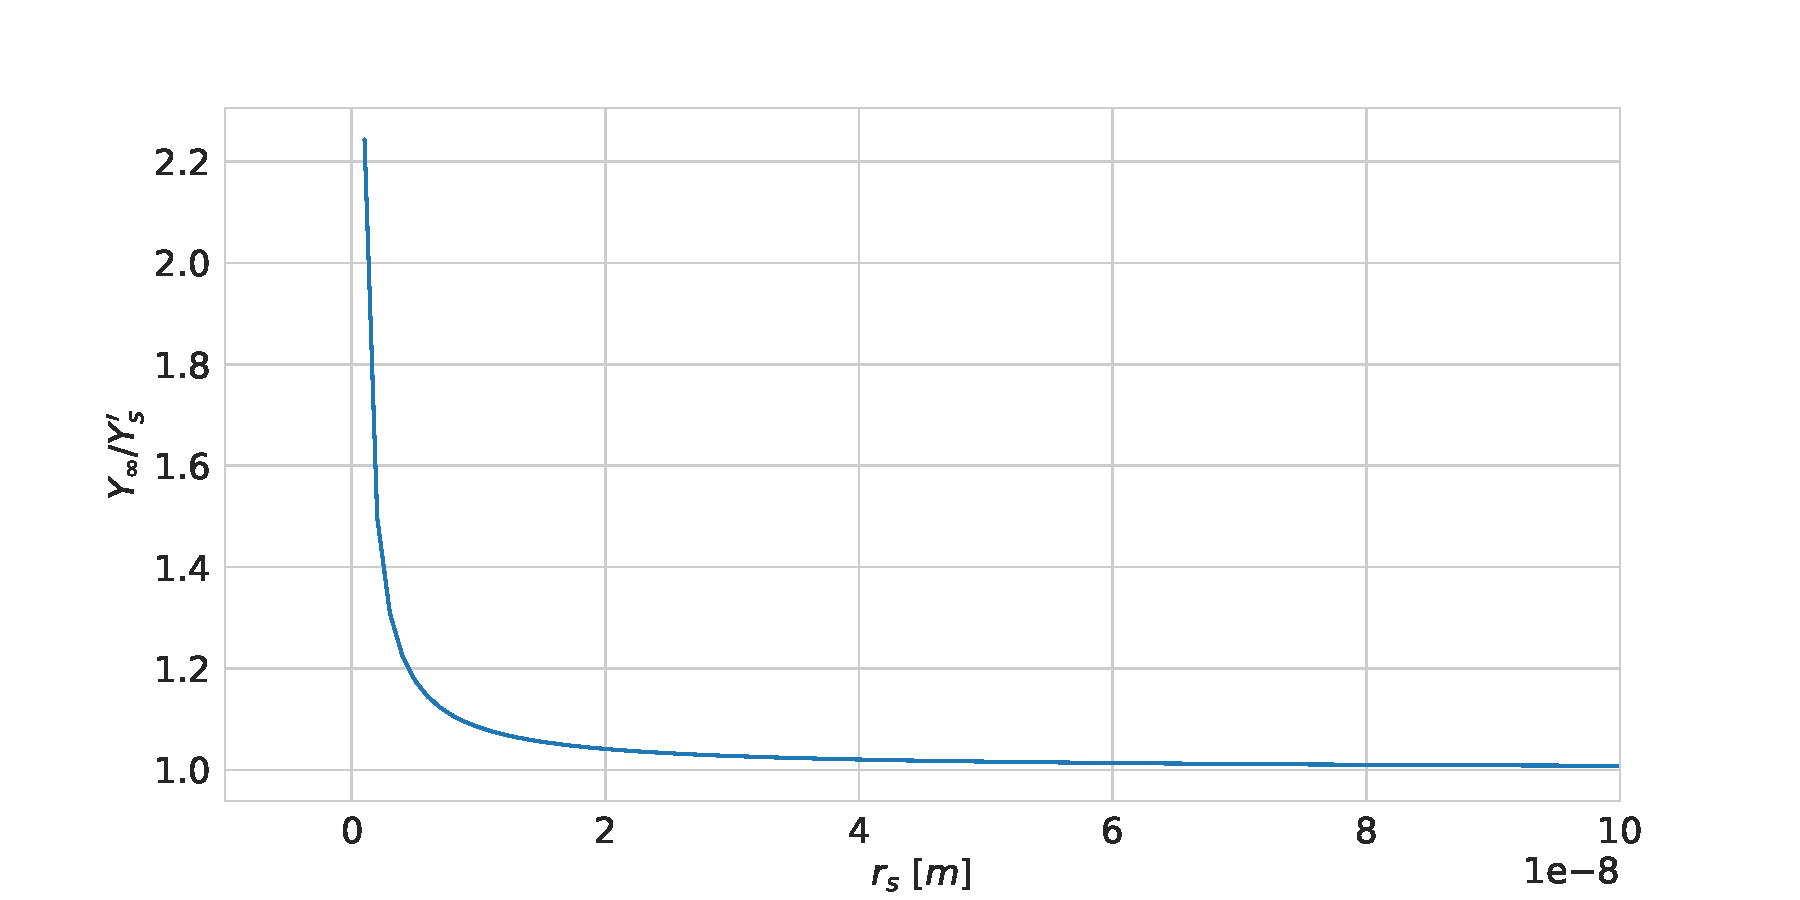
\includegraphics[trim={0 0 0 30},clip,width=1.0\textwidth]{Figures/Kelvin_supersat.pdf}
    \caption{Supersaturation value needed for droplet growth at $T=350 \mathrm{K}$ and $p=25\: \mathrm{kPa}$}
    \label{f:kelvin_supersat}
\end{figure}
The relationship between the heat flux and the mass change is now sought to describe equilibrium conditions i.e. constant temperature for which latent heat is exchanged for mass. For this, the energy equation is first formulated.
\begin{equation}\label{eq:d2_cond_energybalance}
    r^{2}\rho v c_{p}\frac{\partial T}{\partial r}-\frac{\partial}{\partial r}\left(\lambda r^{2}  \frac{\partial T}{\partial r}\right) =0
\end{equation}
As the species conservation equation, Eq. \ref{eq:d2_cond_energybalance} is integrated across the surface. If the transient temperature term is neglected due to equilibrium conditions, the following boundary condition is acquired 
\begin{equation}
    \lambda\frac{\partial T}{\partial r}|_{s}=\rho_{s} v_{s} h_{vl}
\end{equation}
Thus, the energy balance becomes
\begin{equation}
    r_{s}^{2}v_{s}(T_{s}-T+\frac{h_{vl}}{c_{p}})+\hat{\alpha} r^{2}\frac{\mathrm{d}T}{\mathrm{d}r}=0,
\end{equation}
with $\hat{\alpha}=\lambda/c_{p}\rho$. Lastly, the variables are split and the equations are integrated between the interface and a distance infinitely away from the droplet to acquire: 
\begin{equation}\label{eq:d2_cond_energygrowth}
    r_{s}v_{s}=\hat{\alpha}\ln\left(1+\frac{c_{p}(T_{\infty}-T_{s})}{h_{lv}}\right)
\end{equation}
The right term in the logarithmic function can be referred to as the thermal transfer number $B_{T}$. In the case that the Lewis number, \textrm{Le}, representing the proportion between mass and thermal diffusivity, is equal to unity, the equilibrium conditions are reached thus linking thermal and mass transfer:
\begin{equation}
    \begin{aligned}
        \hat{\alpha}\ln(1+B_{T})&=\mathcal{D}\ln(1+B_{M})\Longleftrightarrow B_{T}=B_{M}\\
        \rightarrow  \frac{c_{p}(T_{\infty}-T_{s})}{h_{lv}}&=\frac{Y_{\infty}-Y_{s}}{Y_{s}-1}
    \end{aligned}
\end{equation}
In addition to the found equilibrium conditions, the "Infinite Conductivity" model \cite{abramzon1989droplet} will be introduced to investigate a transient temperature progression of the droplet given an initial condition, until equilibrium is reached. This model assumes that the droplet temperature is still uniform yet time-dependent. With an energy balance, as presented in the Knudsen model (Eq. \ref{eq:knudsen balance}), the convective heat transfer coefficient can be replaced by definition with the Nusselt number, \textrm{Nu}, which represents the proportion of convective to conductive heat transfer. The total heat transferred out of the droplet, $Q_{conv}$, is written as:
\begin{equation}
    Q_{conv}=\pi d\lambda\textrm{Nu}(T_{\infty}-T_{s})
\end{equation}
A convection correction to \textrm{Nu} was introduced by Abramzon and Sirignano due to increased heat transfer in the case of non-quiescent conditions \cite{abramzon1989droplet}. Such a case is not considered in this study, however, it is used for the demonstration of the derivation. Nevertheless, the correction is implemented in the code, although it possesses negligible effects on the results. This is demonstrated in Appendix \ref{s:appendix A}. 
\begin{equation}
    \begin{aligned}
        \textrm{Nu}&=\textrm{Nu*}\frac{\ln(1+B_{T})}{B_{T}} \\
        \rightarrow Q_{conv}&=\pi d\lambda\textrm{Nu*}(T_{\infty}-T_{s})\frac{\ln(1+B_{T})}{B_{T}}
    \end{aligned}
\end{equation}
where \textrm{Nu*} represents the modified Nusselt number defined via empirical correction \cite{abramzon1989droplet}. Lastly, if Eq. \ref{eq:d2_cond_energygrowth} is corrected through \textrm{Nu*}, it can be inserted into the above equation to get the thermal energy transferred to the gas phase. 
\begin{equation}
    Q_{conv}=-\dot m \frac{c_{pg}(T_{\infty}-T_{s})}{B_{T}}
\end{equation}
Rearranging the energy balance (Eq. \ref{eq:knudsen balance}) yields the time derivative of the droplet's temperature. 
\begin{equation}\label{eq:heat_out_droplet}
    Q_{d}=m_{d}c_{pd}\frac{\mathrm{d}T_{d}}{\mathrm{d}t}=-\dot{m}\left(\frac{c_{pg}(T_{\infty}-T_{s})}{B_{T}}-h_{vl}\right)
\end{equation}

The $d^2$ droplet condensation model was written in Python and is presented in Algorithm \ref{alg:droplet}. Following Abramzon and Sirignano \cite{abramzon1989droplet} the "one-third averaging" was used to calculate the physical properties of the vapor phase.
\begin{algorithm}[H]
    \caption{Simplified droplet growth concept}
    \label{alg:droplet}
    \begin{algorithmic}[1]
    \State \textbf{Initialize}: Boundary Conditions: $T_{s}$, $T_{\infty}$, $p$, $r_{0}$ \Comment{$r_{0}$: initial droplet size}
    \State \textbf{Initialize}: $\mathrm{d}t$ 
    \State \textbf{Compute}: $p'$ at $T_{\infty}$\\ 
    \quad \quad \quad \quad \quad $p'_{s}$ at $T_{s}$ \\
    \quad \quad \quad \quad \quad$Y_{s}$ from $p'_{s}$ \& $p$\\
    \quad \quad \quad \quad \quad$Y_{\infty}$ at $T_{s}$ \Comment{Kelvin equation} \\
    
    \quad \quad \quad \quad \quad$m$ from $r_{0}$ \& $\rho_{l}$ \Comment{$m$: initial mass of droplet}
    \For{\emph{total number of iterations} }
    \State \textbf{Compute}: $\rho_{g}$, $c_{p}$, $\lambda_{g}$, $\mu_{g}$, $\mathcal{D}$ \Comment{Using one third law averaging at $T_{s}$ \& $T_{\infty}$}
    \State \textbf{Compute}: $\mathrm{Sh}$, $\mathrm{Nu}$, $\mathrm{Sh^*}$, $\mathrm{Nu^*}$ \Comment{Sherwood and Nusselt numbers. See Appendix \ref{s:appendix A}}
    \State $B_{M}=(Y_{\infty}-Y_{s})/(Y_{s}-1)$
    \State $\dot{m}=-2\pi\rho_{v}\mathcal{D}\cdot r \cdot \mathrm{Sh^*}\cdot \log(1+B_{M})$
    \State $B_{T}=c_{pg}(T_{\infty}-T_{s})/h_{vl}$ \Comment{Value is iteratively corrected using $\mathrm{Sh^*}\: \&\: \mathrm{Nu^*}$}
    \State $Q_{conv}=\dot{m}\cdot (c_{pg}(T_{\infty}-T_{s})/B_{T})-h_{vl}$
    \State $r_{s}=\sqrt[3]{(3/4\pi \rho_{l})\cdot m+\dot{m}\cdot \mathrm{d}t}$
    \State $m=r_{s}^{3}\cdot \rho_{l}\cdot 4\pi/3$
    \State $T_{s}=(6 Q_{conv}\mathrm{d}t)/(c_{pd}(m+\dot{m}\cdot \mathrm{d}t))+T_{s}$
    \State \textbf{Recompute}: $p'_{s}$ at $T_{s}$
    \State \textbf{Recompute}: $Y_{s}$ from $p'_{s}$ \& $p$
    \EndFor
    
    \end{algorithmic}
\end{algorithm}
Similarly to the Knudsen algorithm, thermophysical and transport properties are calculated using various
fitting functions (see Table \ref{t:perry_calcs} Appendix \ref{s:appendix B}).
\subsubsection{Heterogeneous Condensation in Pure Vapor}\label{sss:Methodology-Droplet-het}
Similar to the Knudsen model, the heterogeneous droplet growth rate model presented by Khandekar \cite{khandekar2020drop} is a first-order ODE that can be solved using the RK45 method. The interfacial heat transfer coefficient $h_{int}$ requires special attention due to various values and models found in the literature. The following formulation, derived from molecular dynamics, is often found in the literature:
\begin{equation}
    h_{int}=\frac{2\hat{\sigma}}{2-\hat{\sigma}}\frac{h_{vl}^{2}}{T'v_{vl}}\left(\frac{W_{w}}{2\pi R T'}\right)^{1/2}
\end{equation}
With $v_{vl}$ being the specific volume difference between the two phases. The problem originates from the choice of the accommodation coefficient $\hat{\sigma}$, as it illustrates the fraction of water molecules that heat the interface of the droplet and condense. In fact, the Knudsen model for the homogeneous case developed by Gyarmathy \cite{gyarmathy1962grundlagen} originated due to the difficulties of choosing an accurate $\hat{\sigma}$ under different configurations \cite{gerber2004pressure}. In some respect, the Knudsen number and the accommodation coefficient are two variables that attempt to convey the same information: the number of water molecules that will participate in the condensation process. While Khandekar proposes a value between $0.02-0.04$ for water, yielding $h_{int}\approx 0.3$ $\mathrm{MW/Km}^2$, Marengo and Tanasawa \cite{marengo2022surface} \cite{tanasawa1991advances} report a value around $1$, yielding $h_{int}\approx 16$ $\mathrm{MW/Km}^2$. Liu and Cheng \cite{liu2015dropwise} used a value of $0.3$. The influence of $\hat{\sigma}$ will be presented in Section \ref{s:Results}.

The manner in which the Python code operates is depicted in Algorithm \ref{alg:het}. The ODE is solved iteratively using the RK45 algorithm. 
\begin{algorithm}[H]
    \caption{Heterogeneous Condensation Growth Model}
    \label{alg:het}
    \begin{algorithmic}[1]
    \State \textbf{Initialize}: Boundary Conditions: $T_{wall}$, $T_{\infty}$,$p$, $\theta$  \Comment{$\theta$: depending on surface of interest}
    \State \textbf{Initialize}: $\mathrm{d}t$ \Comment{time step of evaluated points}
    \State \textbf{Compute}: $h_{vl}$ at $p$\\ 
    \quad \quad \quad \quad \quad$T'$ at $T_{\infty}$ \\
    \quad \quad \quad \quad \quad$\sigma$ at $T_{\infty}$ \\
    \quad \quad \quad \quad \quad$\lambda_{l}$ at $T_{\infty}$ \\
    \quad \quad \quad \quad \quad$h_{int}$ at $T_{\infty}$ \\
    \State \textbf{Solve}: $\frac{\mathrm{d}r}{\mathrm{d}t}= \left(\frac{4(T'-T_{w})}{\rho_{l}h_{vl}}\right)(1-\frac{r_{min}}{r})\left(\frac{2}{h_{int}}+\frac{r(1-\cos\theta)}{\lambda_{l}}\right)^{-1}  \cdot\left(\frac{1-\cos\theta}{2-3\cos\theta+\cos^{3}\theta}\right)$ \Comment{RK45}
    \end{algorithmic}
\end{algorithm}
\noindent
The functions used for the calculation of variables such as surface tension and thermal conductivity are presented in Appendix \ref{s:appendix B}.

Lastly, to integrate the product of the heat transfer through the droplet and the population distribution, a simple trapezoidal integration method was utilized. For this, radius values, growth rate values and droplet population values at each time step were saved to allow and accurate evaluation of the integral. 

\subsection{Homogeneous Condensation: Numerical Method}\label{ss:Methodology-Homogeneous}
\subsubsection{Computational Domain}\label{sss:Methodology-homogeneous-Domain}
A 2D mesh of a cylinder was created in OpenFOAM. Because resolving the modes of wake instabilities are not of interest in this study, only half of the domain was created with a symmetry boundary condition to reduce the number of cells and thus reduce computational demands. The total number of cells used in the streamwise direction is $200$, and $30$ in the spanwise direction.   
\begin{figure}[H]
    \centering
    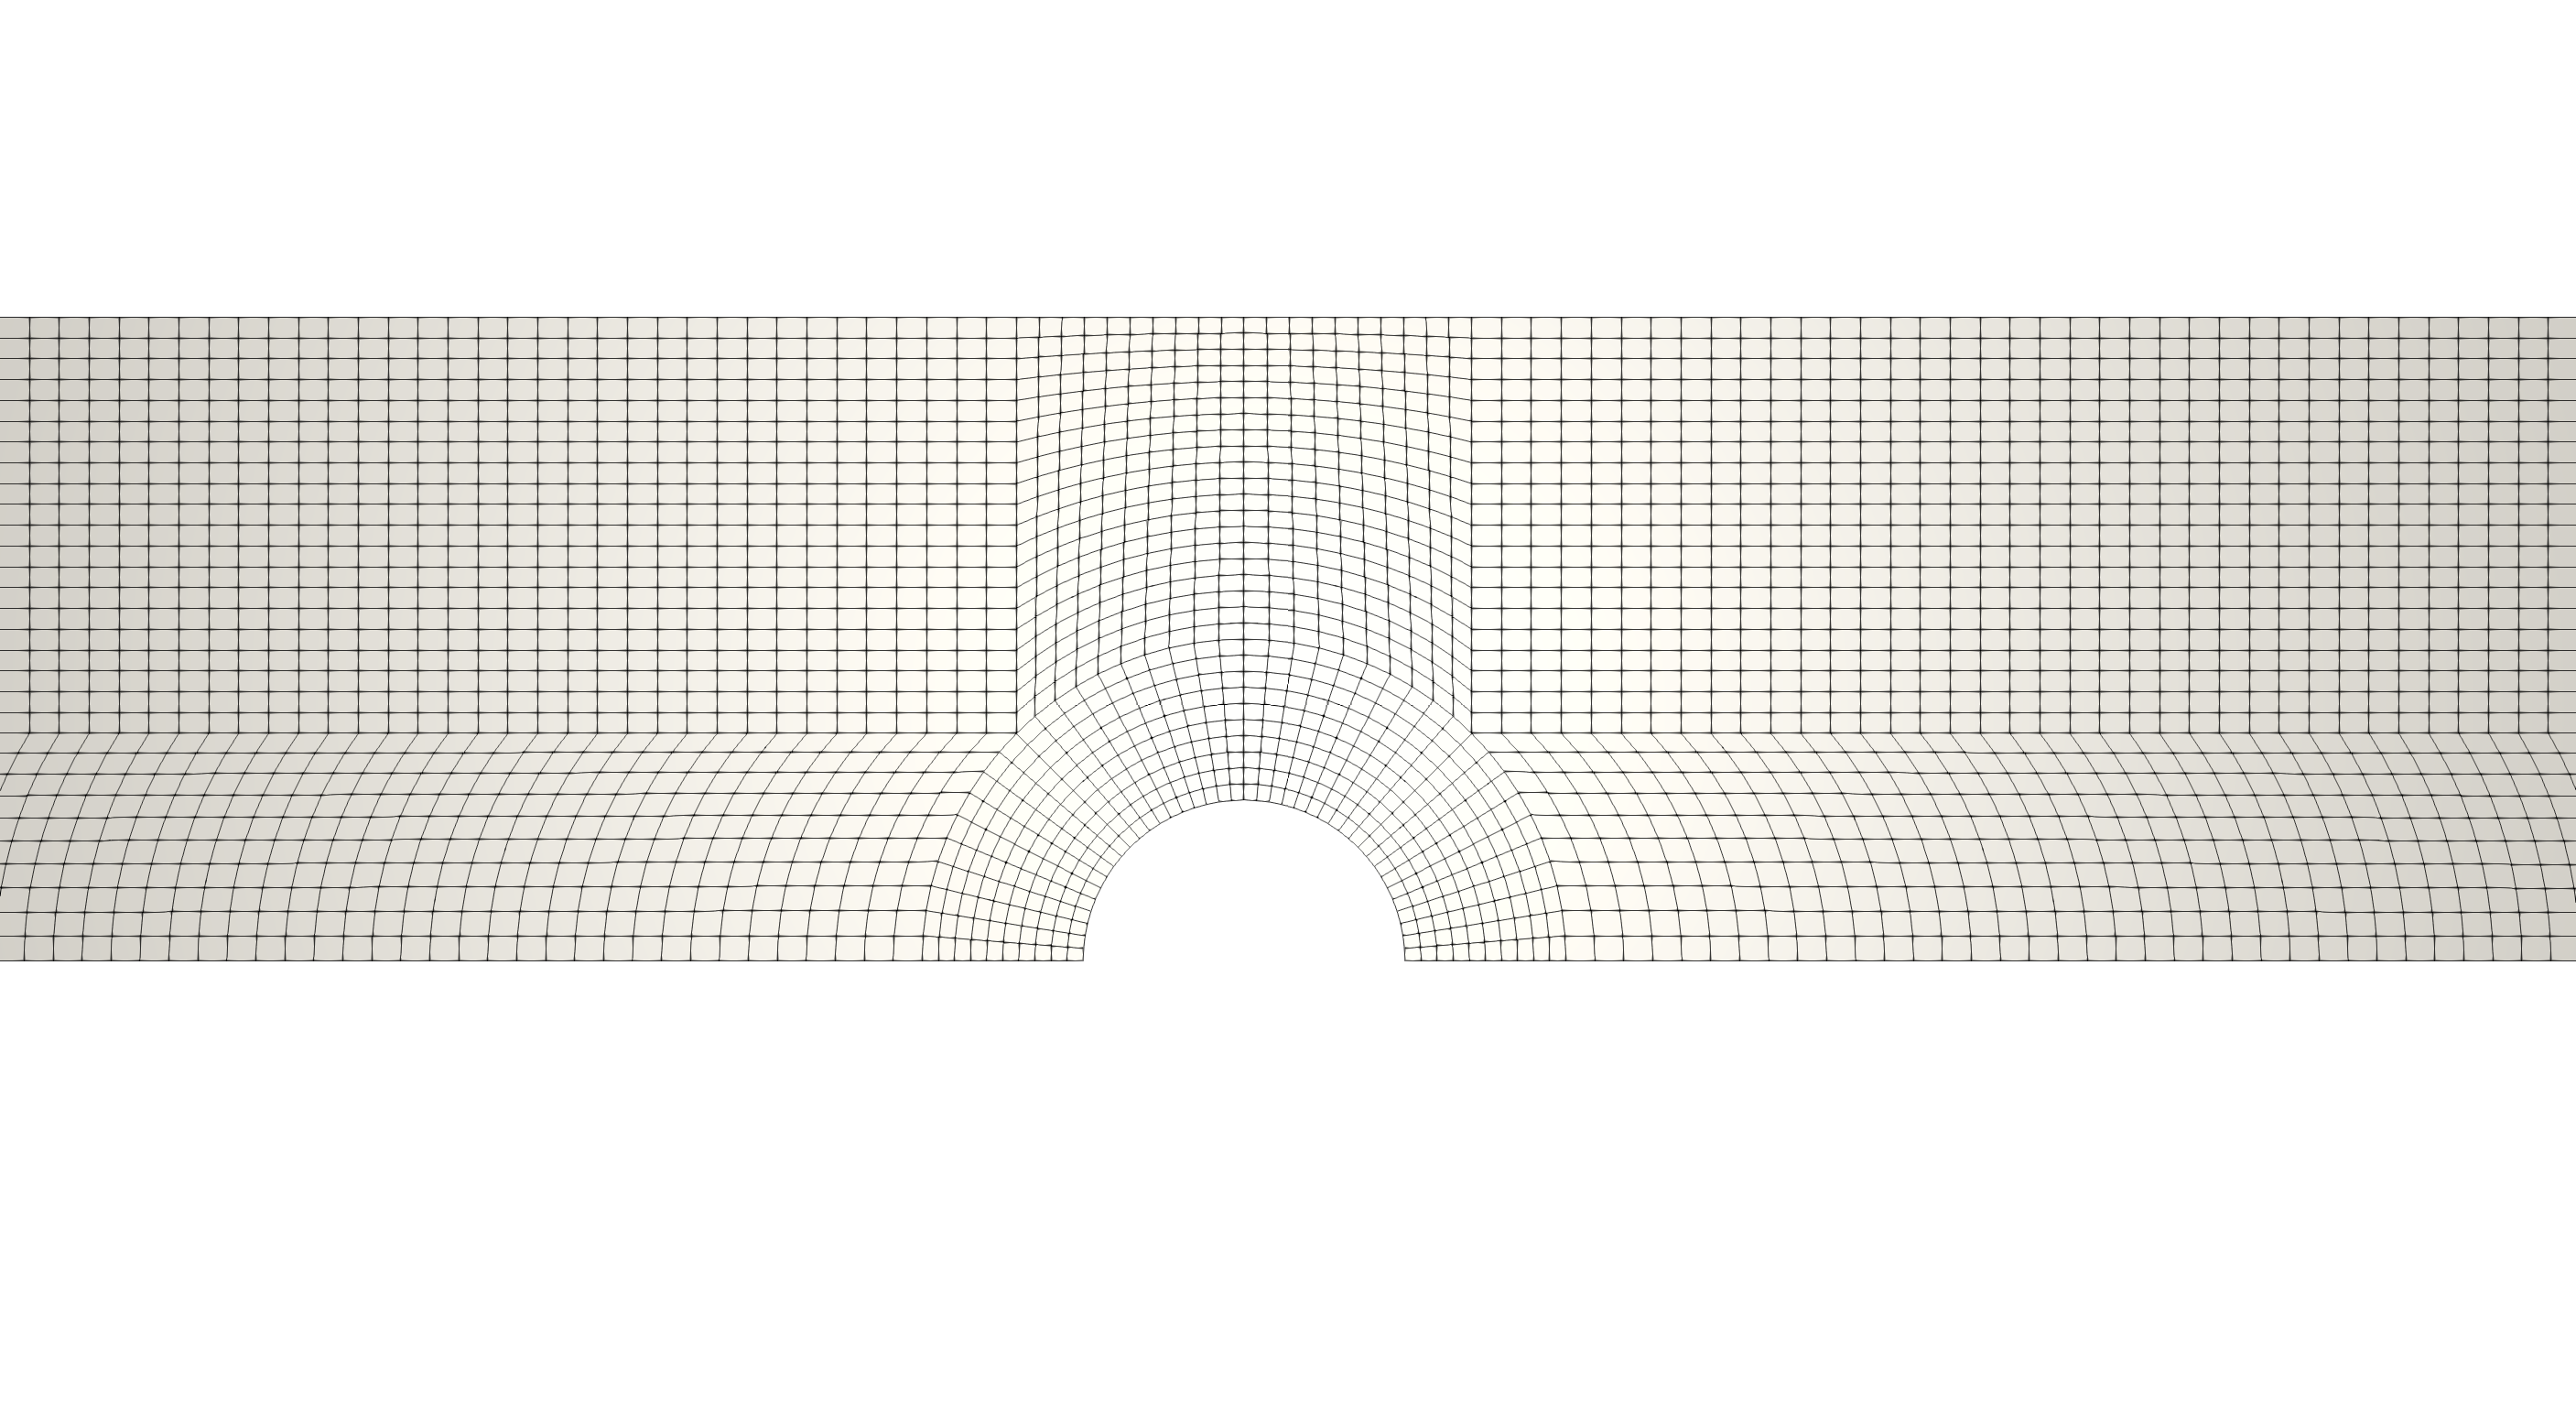
\includegraphics[trim={0 400 0 300},clip,width=1\textwidth]{Figures/Mesh_Cylinder.png}
    \caption{Cylinder mesh }
    \label{f:cylinderMesh}
\end{figure}
\begin{table}[H]
    \centering
    \begin{threeparttable}[b]
    
    % \captionsetup{justification=centering}
    \caption{Boundary Conditions of Cylinder Case}
    \renewcommand{\arraystretch}{1.3}
    \begin{tabular}{||c|c|c|c|c|c||}
    \hline
    \textbf{Variable} & \textbf{Left}& \textbf{Right}& \textbf{Up} & \textbf{Down}& \textbf{Cylinder (Wall)}\\ \hline\hline
     $U \:[\mathrm{m/s}]$&$([50,90,130],0,0)\tnote{1}$&Zero Gradient&Zero Gradient&Symmetry&No Slip\\\hline
     $p \:[\mathrm{Pa}]$&Zero Gradient& $101325$&Zero Gradient&Symmetry&Zero Gradient \\\hline
     $T \:[\mathrm{K}]$&$373$&Zero Gradient&Zero Gradient&Symmetry&Zero Gradient\\ \hline
     $\alpha$&$1$&Zero Gradient&Zero Gradient&Symmetry&Zero Gradient\\\hline
     $\eta\:[\mathrm{1/m^3}]$&$0$&Zero Gradient&Zero Gradient&Symmetry&Zero Gradient\\\hline
     \end{tabular}
     \begin{tablenotes}
        \item [1] Three simulated inlet conditions
    \end{tablenotes}
    \label{t:Cylinder BC}
    \end{threeparttable}
\end{table}
The Boundary conditions for all cylinder simulations are listed in Table \ref{t:Cylinder BC}. Note, that three different inlet velocities are under investigation (depicted in Table \ref{t:Cylinder BC} as square brackets). In doing so, the influence of supercooling on droplet nucleation can be qualitatively demonstrated. Furthermore, it should be mentioned that all three velocities are below a Mach number of $0.3$. The flow configuration is thus very different than that of a steam turbine, where choked conditions are often the case. As a result, high non-equilibrium conditions can't be reached and thus high levels of nucleations will not be observed. The next section will provide details on the nucleation model modifications which will allow the observation of nucleation under such flow configuration. Finally, an upwind scheme was employed to discretize the convective term in the momentum equation, while a limited linear scheme was utilized for handling the convective term in the other transport equations. For the limited linear scheme, a coefficient of $1$ was used which indicates strong limiting of the linear scheme towards upwind at regions of high gradients \cite{greenshields2022}.
\subsubsection{Transport Equations and Condensation Models}\label{sss:Methodology-homogeneous-Transport} 
The transport equations are modeled consistently with those presented by Gerber and Kermani following the Eulerian/Eulerian formulation \cite{gerber2004pressure} (Eqs. \ref{eq:v_conti}-\ref{eq:v_energy}). In addition to these, the $\kappa-\epsilon$ transport equations are used to solve the closure and remain unmodified i.e. no influence from the mass fraction and droplet number. Furthermore, the droplets nucleation and growth model and their respective source term remain unchanged and follow the Knudsen model (Eqs. \ref{eq:nucleation gerber}-\ref{eq:average_radius}). For simplicity, the nucleated droplet temperatures are fixed at the saturation conditions set by the inlet temperature.  However, the critical radius, $r^*$, of nucleation will be modified to enable the nucleation of additional droplets. This is done because substantial non-equilibrium conditions can only be acquired for much larger velocities, such as a transonic flow within a steam turbine, where rapid vapor expansion takes place. Although this would lead to an unphysical number of droplets under such conditions, the dependency of the temperature on the nucleation rate and droplet count can be qualitatively evaluated. The level of supersaturation, $S$, is computed as follows:
\begin{equation}
    S=\frac{p}{p'(T_{v})}+1
\end{equation}
where the saturation pressure is calculated using the Clasius-Clapeyron equation. As the flow accelerates around the cylinder, its temperature will sink consistently following the first law of thermodynamics. $p$ on the other hand, should be determined by extrapolating the isotherm into the dome (metastable extensions) and thus acquiring a higher static pressure than the saturation value \cite{gerber2004pressure}. However, this feature was not incorporated into the solver because the research project's primary focus does not entail a quantitative examination of this specific flow configuration. The fundamental physics governing the flow should remain unchanged even when artificially increasing the supersaturation. Nevertheless, $p'$ will decrease faster than the reduction of the static pressure due to the increase in velocity, and supersaturation will be achieved. Thus, for each supersaturation level acquired, $1$ will be added to increase the sensitivity of nucleation.

Because the temperature range is relatively small, thermophysical properties such as viscosity, surface tension, liquid density and latent heat were assumed constant and defined according to the inlet conditions. The density was determined by the Peng Robinson model, a two-constant equation of state, given by OpenFOAM, with critical values for steam \cite{pengrobinson}.  
\subsection{Heterogeneous Condensation: Numerical Method}\label{ss:Methodology-Heterogeneous}

\subsubsection{Computational Domain}\label{sss:Methodology-Heterogeneous-Domain}
A basic 3D flat plate in a quiescent domain may not give the most accurate depiction of a flow within a condenser, nevertheless, the physics involved are similar enough to allow a quantitative comparison of wall heat flux with values found in the literature. The domain for the coarse mesh is illustrated in Figure \ref{f:flatplate_Mesh} and the respective boundary conditions in Table \ref{t:flatplate BC}. For the coarse mesh, $20\times 4$ (length $\times$ depth) cells were used for the wall patch and $10$ cells for the height, with an expansion ratio of $4$ away from the wall. Domain dimensions are $20\times 4\times 10$ (length $\times$ depth $\times$ height)  
\begin{figure}[H]
    \centering
    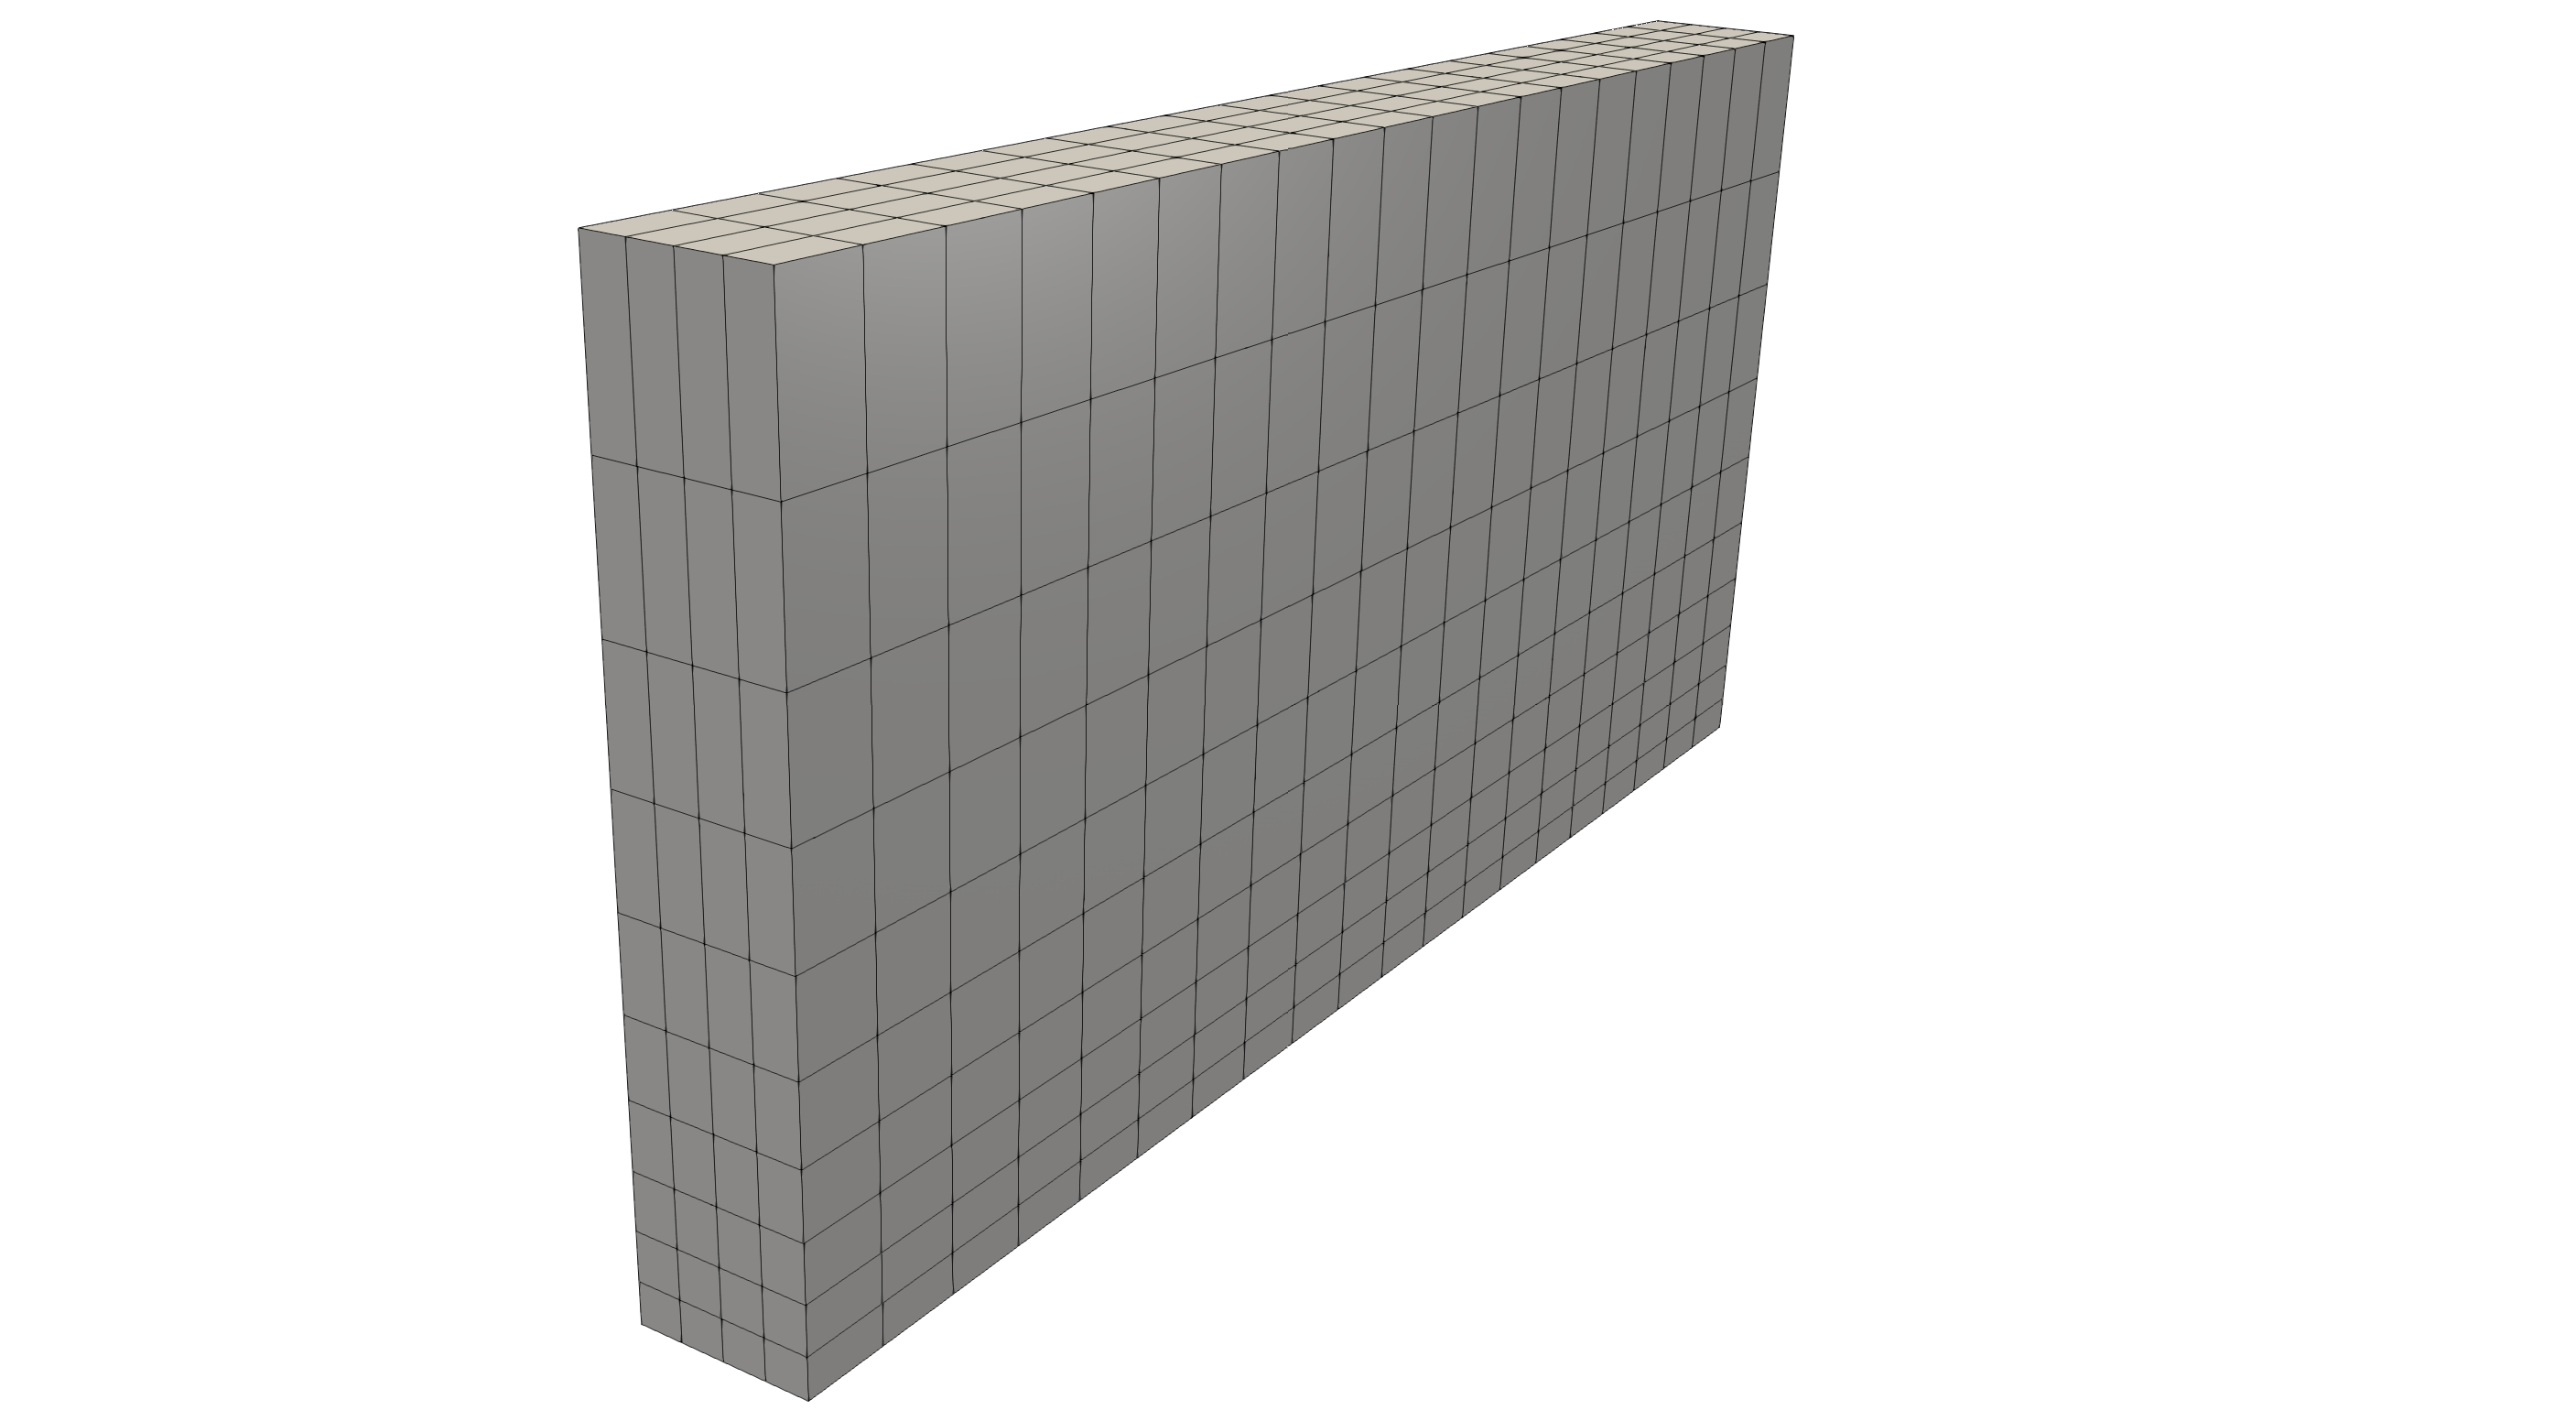
\includegraphics[trim={50 0 200 20},clip,width=0.75\textwidth]{Figures/FlatPlate_Mesh.png}
    \caption{Flat plate mesh }
    \label{f:flatplate_Mesh}
\end{figure}
It was found that refinement of the wall surface area does not have any influence on the results. Therefore, refinement of the mesh was only performed in the height direction. In this case, $200$ cells between the wall and free stream ("up" boundary) with the same expansion rate were used. Lastly, the divergence discretization was performed using the linear upwind for the velocity and limited linear for the other transport equations. However, it is noted that this does not pose great significance due to the domain being quiescent (no flow velocity).   
\begin{table}[H]
    \centering
    \begin{threeparttable}[b]
    
    % \captionsetup{justification=centering}
    \caption{Boundary Conditions of Cylinder Case}
    \renewcommand{\arraystretch}{1.3}
    \begin{tabular}{||c|c|c|c|c|c||}
    \hline
    \textbf{Variable} & \textbf{Left}& \textbf{Right}& \textbf{Up} & \textbf{Down (Wall)}& \textbf{Front and Back}\\ \hline\hline
     $U \:[\mathrm{m/s}]$&No Slip&No Slip&No Slip&No Slip&No Slip\\\hline
     $p\: [\mathrm{Pa}]$&Zero Gradient& Zero Gradient&$101325$&Zero Gradient&Zero Gradient \\\hline
     $T\: [\mathrm{K}]$&Zero Gradient&Zero Gradient&$373$&$367-372$ \tnote{1}&Zero Gradient\\ \hline
     $\alpha$&Zero Gradient&Zero Gradient&$1$&Zero Gradient&Zero Gradient\\\hline
     $\eta\: [1\mathrm{/m}^3]$&Zero Gradient&Zero Gradient&$0$&Zero Gradient&Zero Gradient\\\hline
     \end{tabular}
     \begin{tablenotes}
        \item [1] Vapor-wall temperature difference: $\mathrm{d}T=[1,2,4,6]$
    \end{tablenotes}
    \label{t:flatplate BC}
    \end{threeparttable}
\end{table}
It should be noted that the "up" boundary conditions for $\alpha$ and $\eta$ are unnecessary, due to nucleation source terms that appear only in the wall first cell. Nevertheless, they were fixed for consistency purposes only. Furthermore, $\mathrm{d}T$ values are chosen following values presented by Liu and Cheng \cite{liu2015dropwise}.
\subsubsection{Transport Equations and Condensation Models}\label{sss:Methodology-Heterogeneous-transport}
Consistent with the homogeneous case, the transport equations are modeled following the Eulerian/Eulerian formulation \cite{gerber2004pressure} (Eqs. \ref{eq:v_conti}-\ref{eq:v_energy}). Due to the simulation being unsteady to capture the time progression of the boundary, the source terms require special attention to avoid excessive nucleation on the boundary. This would be the case for a quiescent flat plate configuration because the droplets are not transported away from a nucleation site to allow further nucleation. Therefore, nucleation will accumulate with each time step and yield unphysical results. For instance, for a total simulation time of $t_{total}=10\mathrm{s}$ and an iterative timestep of $\mathrm{d}t=10^{-4}\mathrm{s}$ the nucleation rate is defined as follows 
\begin{equation}\label{eq:sim_nucleation_process}
    J_{d}=\frac{1}{t_{total}}\cdot\mathrm{d}t\cdot N_{s}\frac{A_{cell}}{V_{cell}} =0.1\cdot10^{-4}\cdot N_{s}\frac{A_{cell}}{V_{cell}}
\end{equation}
In terms of physical aspects, this implies that in every simulated second, one-tenth of a droplet forms, and during this second, the formed droplet is further portioned, which is determined by the chosen timestep. 

Since only rectangular cuboid cells were utilized in the case of the flat plate, it can be deduced from Equation \ref{eq:sim_nucleation_process} that the fraction of cell surface area, denoted as $A_{cell}$, and its volume, denoted as $V_{cell}$, are inversely proportional to the cell height. Given that the distribution density provides the number of droplets per unit surface area, it can be reasonably assumed that simulating a one-dimensional problem (with one cell in the length and depth directions) should yield equivalent results to those obtained across the entire domain (as depicted in Figure \ref{f:flatplate_Mesh}), provided that the cell height remains consistent. This assumption was subsequently verified, leading to the utilization of fewer wall cells in the finer mesh simulations.  

For the droplet growth source term, $S_{d}$, several modifications need to be made due to the droplet volume being a function of $\theta$. The average mass and thus radius of a droplet is defined as follows
\begin{equation}
    \begin{aligned}
        \bar{m}=\frac{\alpha}{\eta}\rho_{v}&=\rho_{l}\frac{\pi \bar{r}^{3}}{3}(2-3\cos(\theta)+\cos^{3}(\theta))\\
        \rightarrow \bar{r}&=\left[\frac{3\alpha\rho_{v}}{\rho_{l}\eta\pi(2-3\cos(\theta)+\cos^{3}(\theta))} \right]^{1/3} 
    \end{aligned}
\end{equation}
Compared to the homogeneous case, the average radius would be smaller due to its smaller volume. $\bar{r}$ may be then inserted to Eq. \ref{eq:het_droplet_growth} to acquire the growth rate. Once calculated, $S_{d}$ can be inserted as a source term. Gerber and Kermani \cite{gerber2004pressure} describe $S_{d}$ by considering the mass growth rate of a droplet of size $\bar{r}$ with $\eta$ being the total number of droplets per unit volume of the vapor. Therefore, derived from its general form, one obtains the following
\begin{equation}
    S_{d}= \eta\frac{\mathrm{d}\bar{m}}{\mathrm{d}t}=\eta\rho_{l}\pi\bar{r}^{2}(2-3\cos(\theta)+\cos^{3}(\theta))\frac{\mathrm{d}\bar{r}}{\mathrm{d}t}
\end{equation}
The heat transfer through a single droplet, $Q_{d}$, can be calculated by definition of the mass rate of change
\begin{equation}
    Q_{d}=h_{vl}\frac{\mathrm{d}\bar{m}}{\mathrm{d}t}=h_{vl}\rho_{l}\pi\bar{r}^{2}(2-3\cos(\theta)+\cos^{3}(\theta))\frac{\mathrm{d}\bar{r}}{\mathrm{d}t}
\end{equation}

Integrating the product of $Q_{d}$ with the droplet population distribution $N(r)$ to acquire the wall heat flux can be challenging using numerical methods such as the trapezoidal rule, due to the nature of the simulation: It will be shown in Section \ref{s:Results} that the calculated averaged radius and thus its rate of change will yield good results once the initial growth period is complete. Therefore, integration with respect to $r$ will result in inaccurate wall heat flux. It is thus proposed that the integration will be done analytically with the use of an additional assumption.

By assuming $\mathrm{d}\bar{r}/\mathrm{d}t$ as constant with respect to $\bar{r}$, an obvious error will be made in the integration. Nevertheless, it will be shown that this assumption can hold well for small $\mathrm{d}T$. The analytical integration can then be easily performed. A step-by-step demonstration can be found in Appendix \ref{s:appendix A}.
\begin{equation}\label{eq:wall_heat_flux_analytical}
        q=\frac{h_{vl}\rho_{l}(2-3\cos(\theta)+\cos^{3}(\theta))}{(r_{max})^{\frac{1}{3}}}((r_{max})^{\frac{1}{3}}-(r_{min})^{\frac{1}{3}})\frac{\mathrm{d}\bar{r}}{\mathrm{d}t}
\end{equation}
The simulation will not attempt to depict the departure of droplets from the surface due to their weight. $r_{max}$ can nevertheless be calculated from a basic force balance and will be used as the upper limit of the integration. Khandekar \cite{khandekar2020drop} provides a basic derivation and the resulting equation is a function of the contact angle, the density of the liquid and vapor, surface tension and the gravitational acceleration constant. 


\newpage
\section{Results}\label{s:Results}
In this section, the outcomes displayed encompass the Python code outputs used to address droplet growth models, along with the results obtained from the two OpenFOAM solvers, which simulate nucleation and growth phenomena.

The section will showcase the three droplet growth models (comprising two homogeneous models and one heterogeneous model) in a comparative manner, allowing the assessment of their behaviors under analogous conditions. These findings can offer enhanced insights for interpreting data generated by the OpenFOAM solver, and potentially provide an estimate of the feasibility of incorporating the $d^2$ model into future solver implementations.

Initially, the CNT nucleation model and Knudsen droplet growth were integrated into OpenFOAM to validate the model's reliability qualitatively. Adhering to the same modeling principles, a heterogeneous condensation solver was developed with the aim of obtaining results that align quantitatively with values documented in existing literature.  
\subsection{Droplet Growth: Parametric Analysis and Comparison}\label{ss:Dropwise-D2-Knudsen}
\subsubsection{Homogeneous Droplets}\label{sss:Results-homogeneous-droplets}
At first, the three homogeneous cases will be presented side by side, as some degree of similarity is expected for the same boundary conditions. For this, the domain is fixed at a temperature of $T_{\infty}=350 \mathrm{K}$ for the $d^{2}$ models and $T_{\infty}=373 \mathrm{K}$ for the Knudsen model, while the temperature of the droplets will vary to establish a difference. If the $d^{2}$-law was fixed at $373\mathrm{K}$, it would suggest that the domain is pure vapor thus defeating the purpose of the model. $\mathrm{d}T$ is fixed consistently, therefore, individual temperature values should not have significance regarding the driving force of the process. Notwithstanding, values such as density, viscosity, conductivity, heat capacity and more are a direct function of the temperature, therefore the results may not lead to a quantitative comparison between the models. This comparison is also made difficult due to the pressure and thus latent heat being different for each simulation (due to different $T'$). Trends may still be observed and conclusions regarding the physical nature of the results may still be drawn.  
\begin{figure}[H]
    \centering
    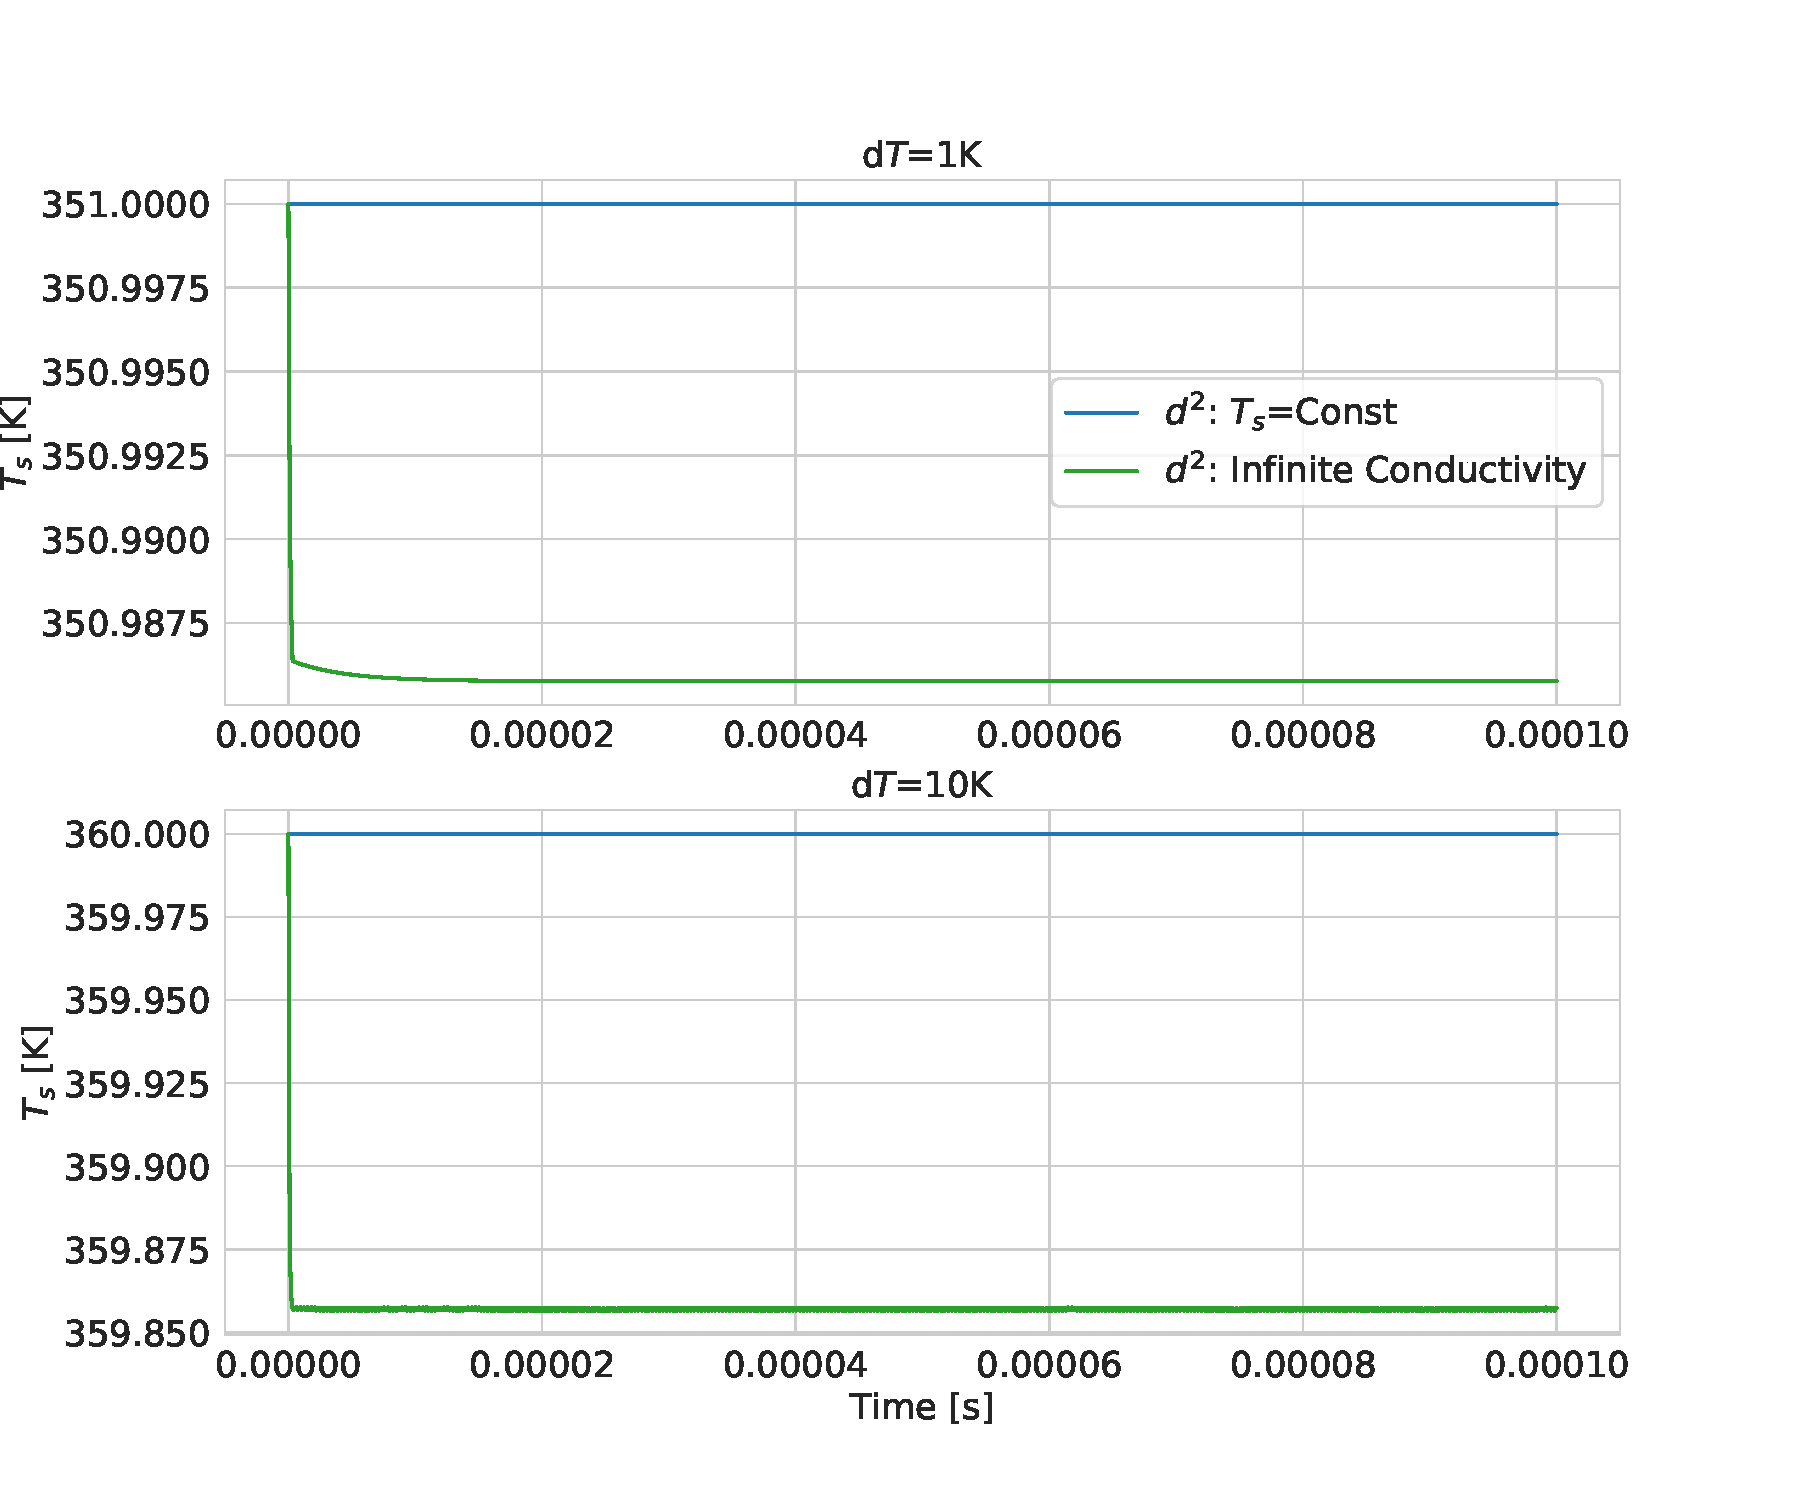
\includegraphics[trim={0 30 0 30},clip,width=1.0\textwidth]{Figures/D2_dT.pdf}
    \caption{$d^{2}$ droplet temperature time progression for two gas-liquid temperature differences.}
    \label{f:dT_hom_vs_D2}
\end{figure}
The progression of the droplet temperature with the infinite conductivity model was inspected to acquire a better understanding of the time scale to reach equilibrium and the value to which the droplet would converge. The findings are presented in Figure \ref{f:dT_hom_vs_D2}. It can be seen that the time to reach the equilibrium temperature is very small. The value to which the temperature converges is for obvious reasons still larger than the ambient, nevertheless, for $\mathrm{d}T=10\mathrm{K}$, the droplet still does not cool down more than $1\mathrm{K}$. This can be explained by the nature of the boundary conditions:  The supersaturation level of the ambient dictated by the Kelvin equation (Eq. \ref{eq:kelvin}) is fixed for the initial droplet temperature.  

Consequently, as the droplet cools with each iteration, the mass fraction at the droplet surface decreases with the saturation pressure (the boundary condition at the droplet surface). As a result, the mass transfer parameter $B_{M}$ and thermal transfer parameter $B_{T}$ will increase and decrease respectively until they are equal for equilibrium to be established. Thus, given the level of supersaturation, established by $\mathrm{d}T$, the droplet temperature will adapt to fulfill the imposed conditions for an equilibrium state. The change in droplet temperature hence does not necessarily need to be scaled with an increase in $\mathrm{d}T$. Illustrating the radius during this initial transient time can reveal further information about their relationship.
\begin{figure}[H]
    \centering
    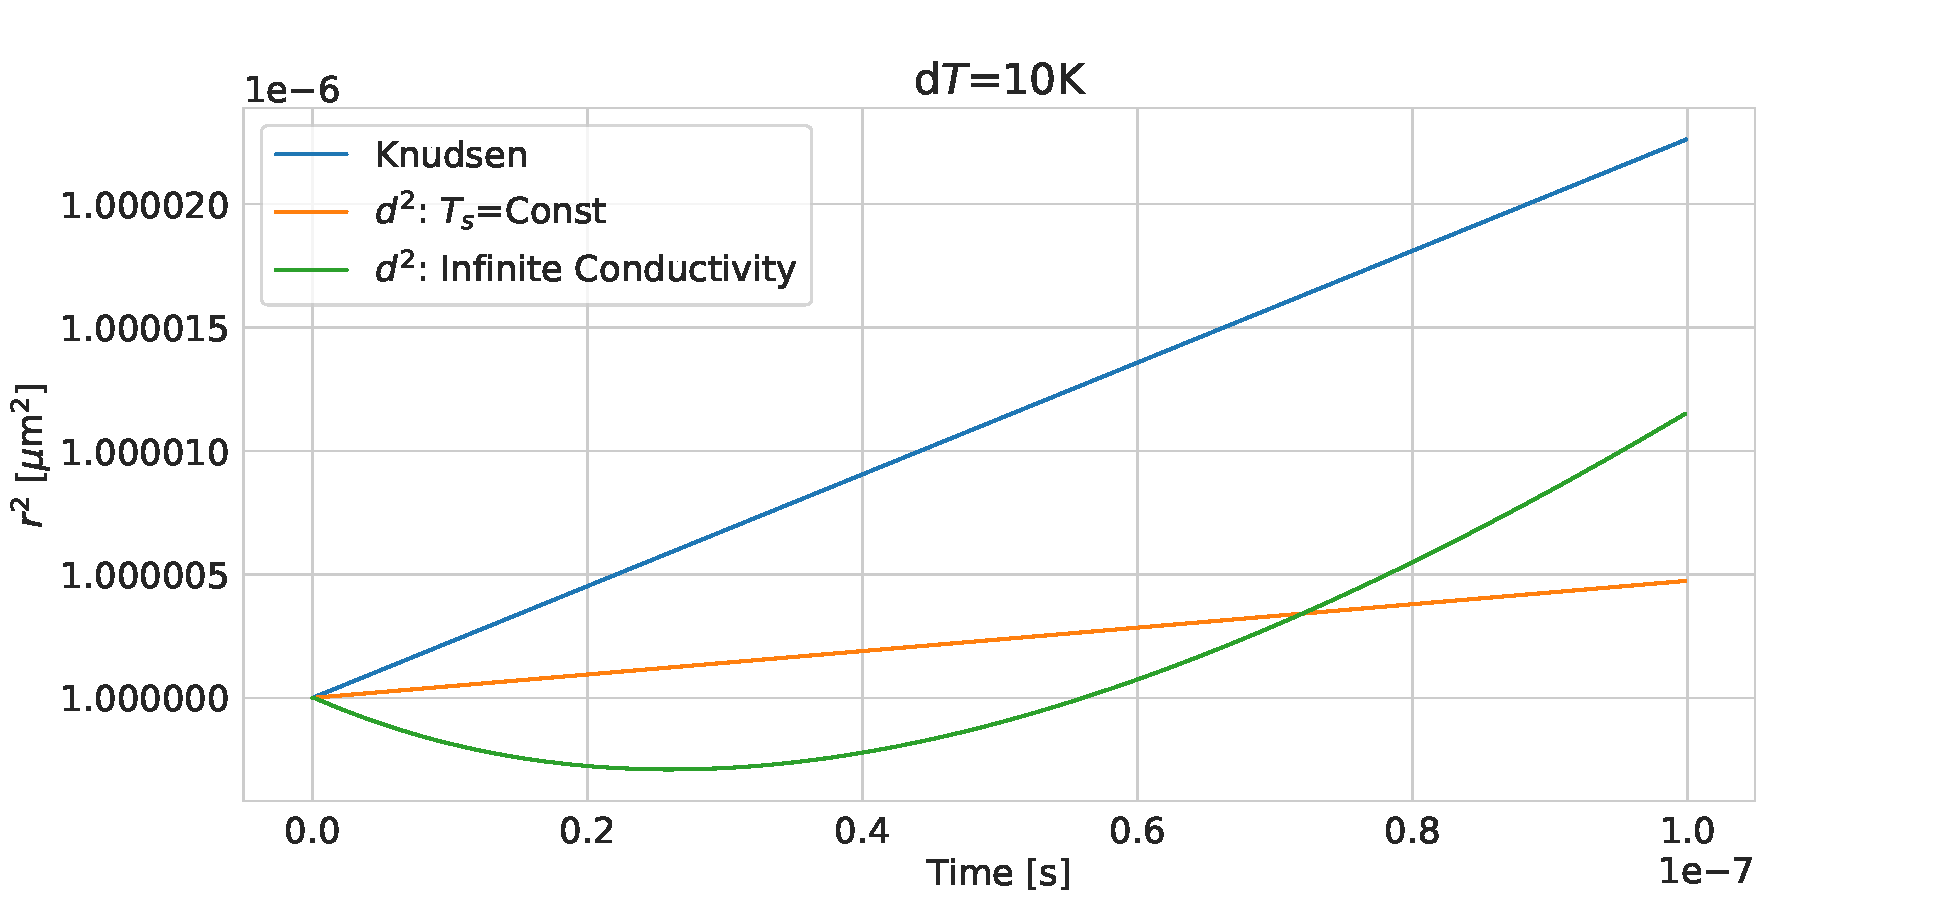
\includegraphics[trim={0 0 0 30},clip,width=1.0\textwidth]{Figures/r_sq_transient_initial.pdf}
    \caption{Droplet squared radius time progression enlarged initial transient state.}
    \label{f:transient_hom_vs_D2}
\end{figure}
Figure \ref{f:transient_hom_vs_D2} illustrates the time progression of the squared droplet radius. It is clear that the Knudsen model and the $d^{2}$ model with constant $\mathrm{d}T$ scale linearly when squaring the radius. Interestingly, the infinite conductivity model suggests that the droplet evaporates initially, and then progresses to grow quicker than the two other models. This initial transient period originates presumably through the strict boundary conditions given to the code. The temperature drop observed in Figure \ref{f:dT_hom_vs_D2}, related to the finding of the equilibrium conditions may be the cause of the initial radius drop.
\begin{figure}[H]
    \centering
    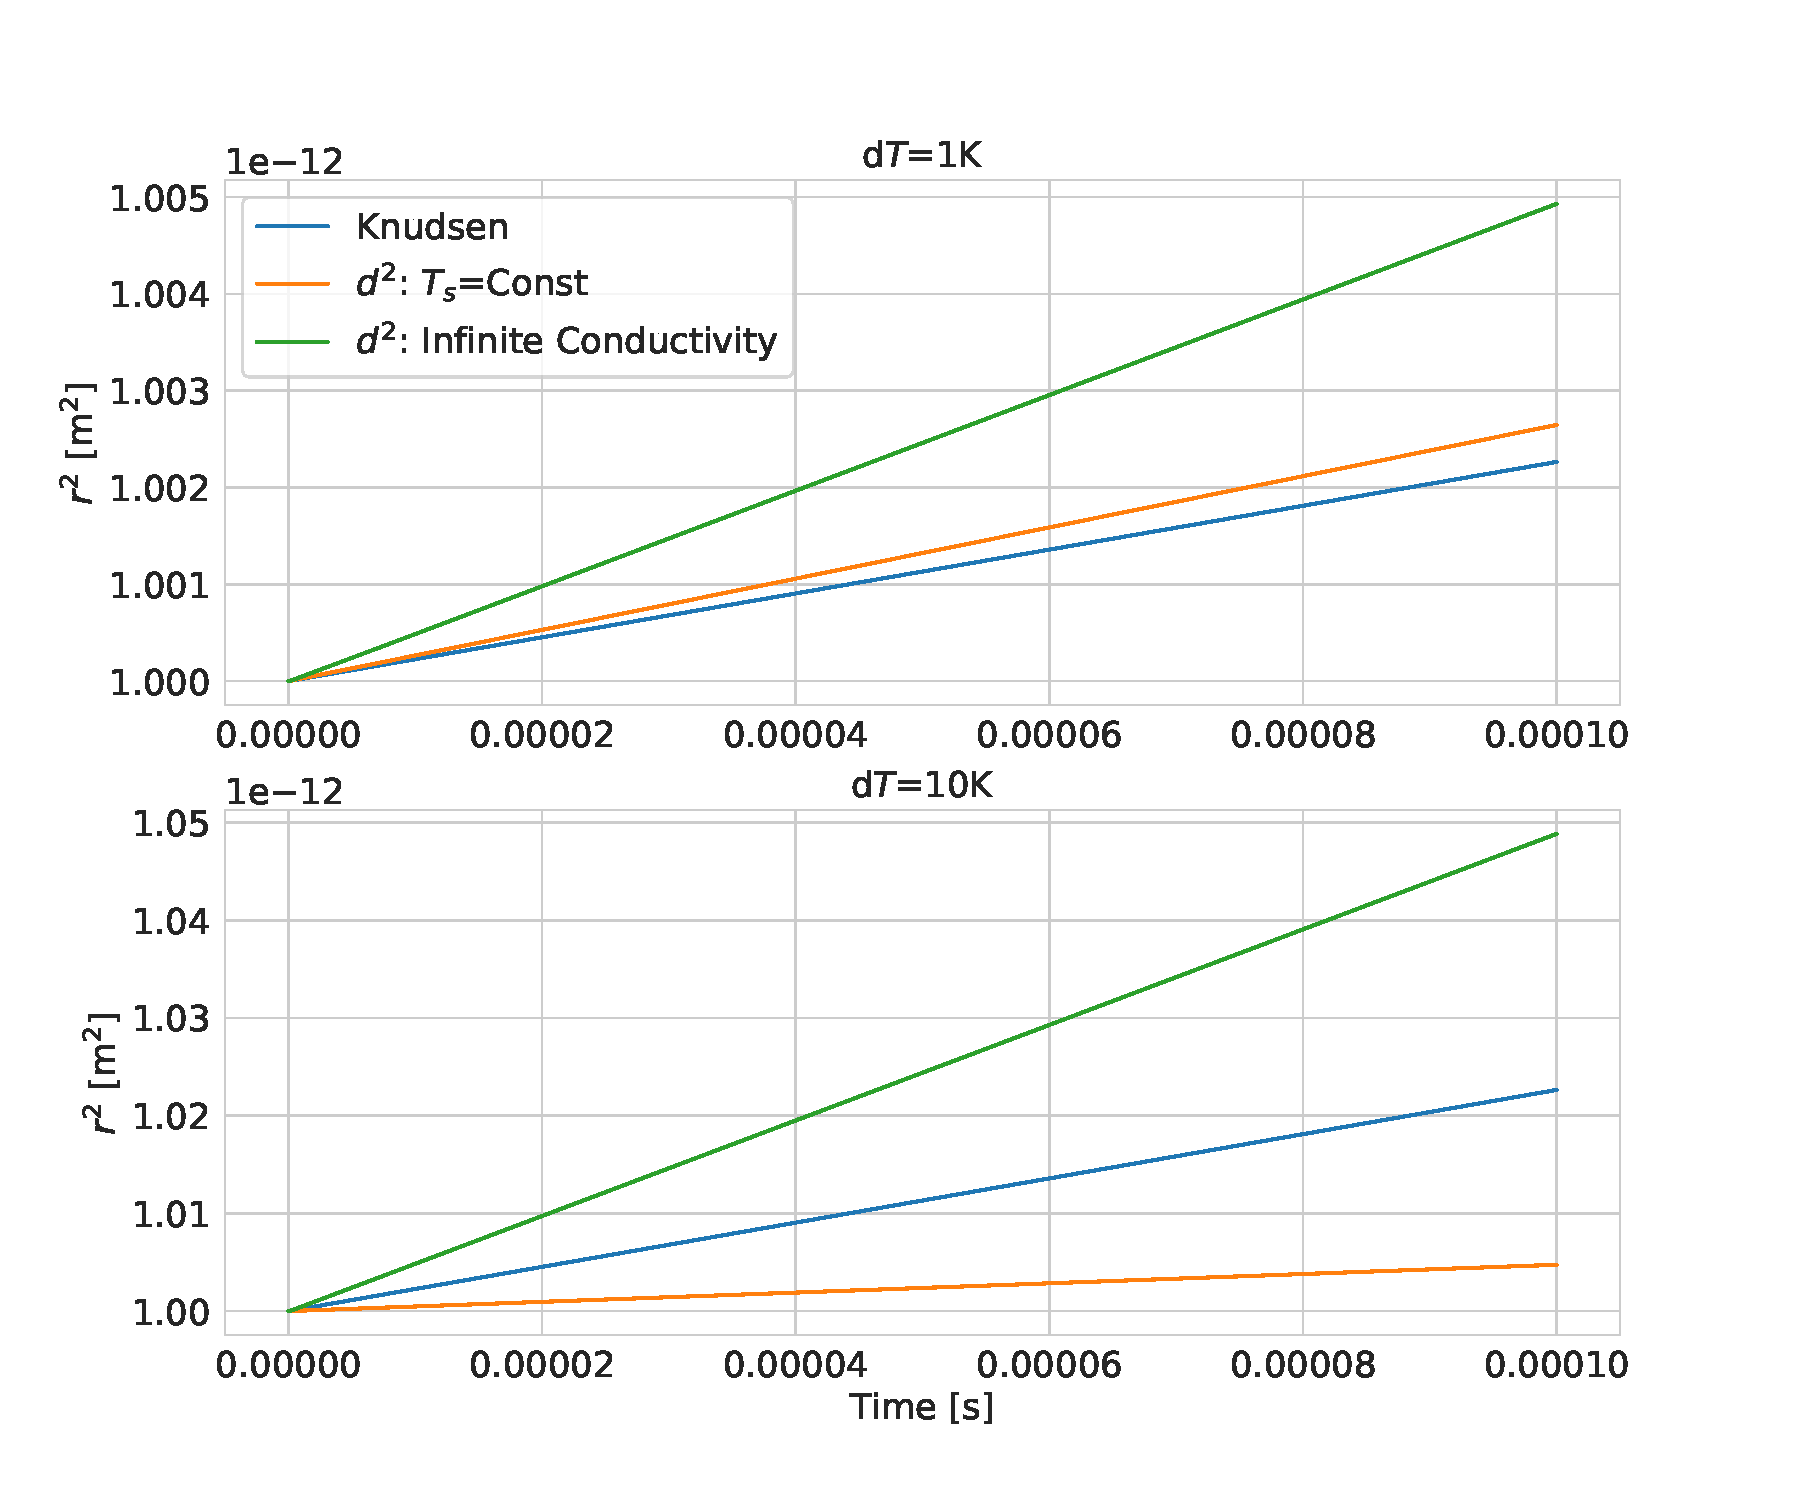
\includegraphics[trim={0 30 0 40},clip,width=1.0\textwidth]{Figures/r_sq_hom_vs_D2_lin.pdf}
    \caption{Droplet squared radius time progression for two gas/vapor-liquid temperature differences.}
    \label{f:r_sq_hom_vs_D2}
\end{figure}
On a larger time scale (Figure \ref{f:r_sq_hom_vs_D2}) it is clear that all models consistently exhibit linear behavior. While the infinite conductivity and Knudsen models scale accordingly when increasing the initial temperature difference, holding the droplet temperature constant for the $d^{2}$ model seems to make the model significantly less sensitive to $\mathrm{d}T$.

To a certain extent, this outcome is predictable as the model doesn't consider thermal interactions, resulting in the problem being entirely dependent on concentration differences at non-equilibrium conditions. In contrast, the Knudsen model, whose driving force is only characterized by the temperature difference, scales appropriately.
\begin{figure}[H]
    \centering
    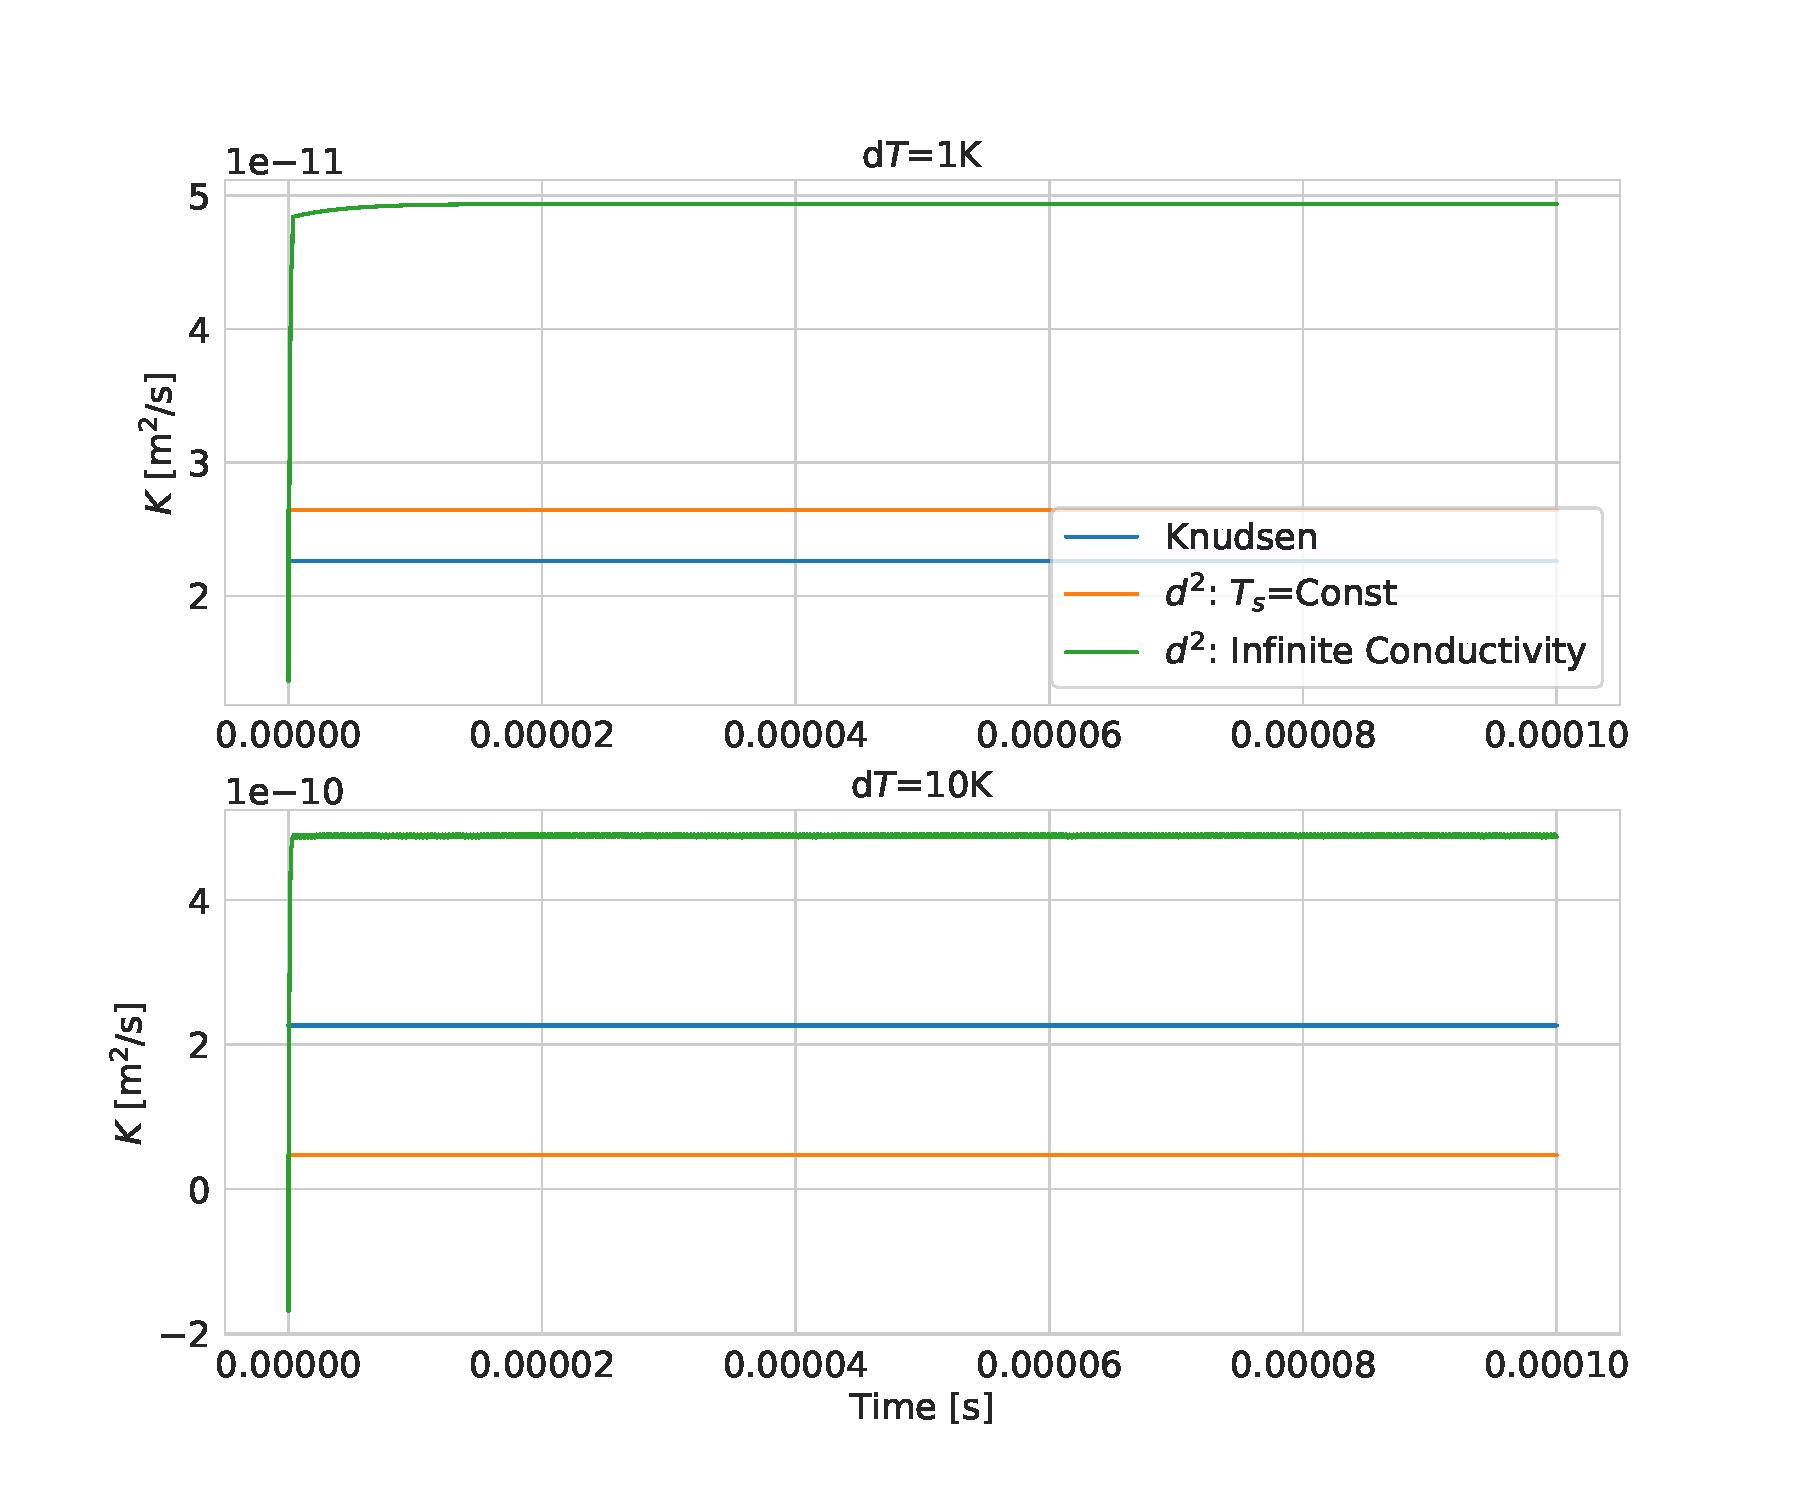
\includegraphics[trim={0 30 0 40},clip,width=1.0\textwidth]{Figures/k_sq_hom_vs_D2.pdf}
    \caption{Droplet squared radius time derivative, $K$, time progression for two gas/vapor-liquid temperature differences.}
    \label{f:K_hom_vs_D2}
\end{figure}
The linearity of the squared radii can be further demonstrated by observing its time derivative. Figure \ref{f:K_hom_vs_D2} illustrates that all three models possess constant growth rates for their squared diameters. Moreover, $K$ scales consistently with $\mathrm{d}T$ as observed in the $r^{2}$ curves. 
\subsubsection{Heterogeneous Droplets}
Because of the relatively higher complexity of dropwise condensation due to the interaction with the surface, several variables are varied at first to assess their influence on the nature of the growth. The contact angle, $\theta$, is of interest as it characterizes the affinity of water molecules to the material of the surface. In Figure \ref{f:dropwise theta change}, a contact angle in the range of $30^{\circ}-120^{\circ}$ are plotted for $\mathrm{d}T=1\mathrm{K}$.
\begin{figure}[H]
    \centering
    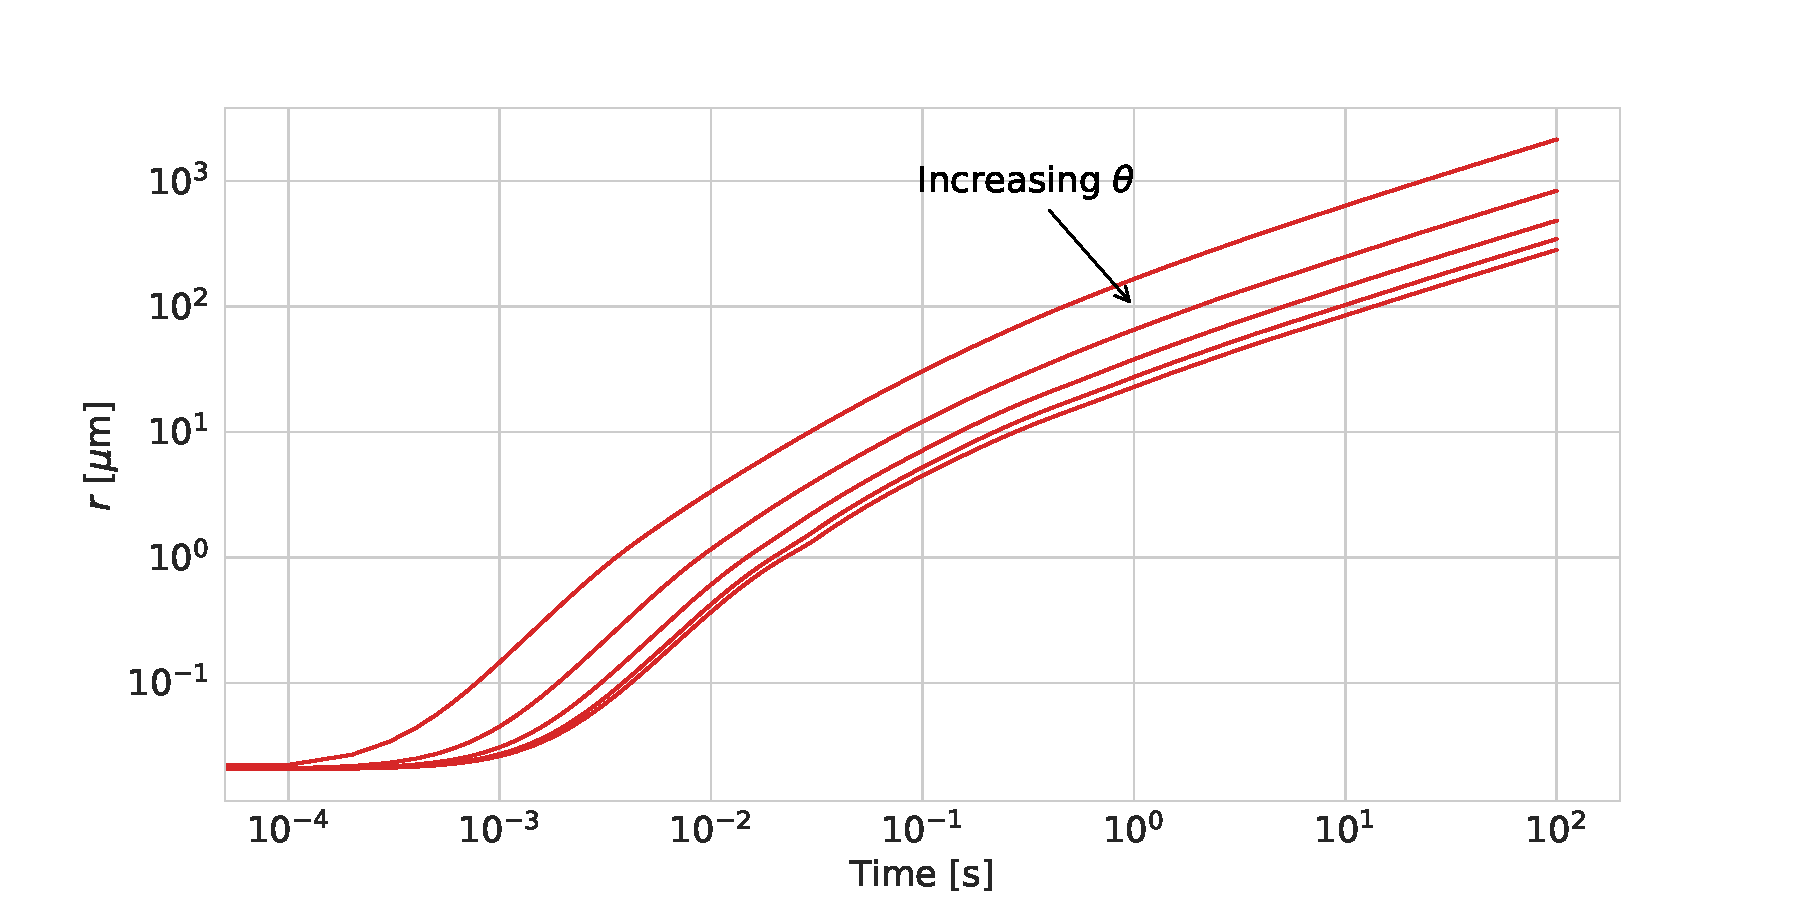
\includegraphics[trim={0 0 0 40},clip,width=1.0\textwidth]{Figures/dropwise_theta.pdf}
    \caption{Dropwise condensation of a single droplet for different contact angles}
    \label{f:dropwise theta change}
\end{figure}
The results show remarkable agreement with data presented by Marengo \cite{marengo2022surface}: The droplets grow in an "S" shaped manner and then tend to a linear curve (in this log-log representation) while remaining relatively parallel to each other. The most prominent observation involves the slowed growth for various angles. As the surface becomes more hydrophilic, the time delay decreases, leading to a shorter duration to achieve a specific radius. Marengo explains this observation by attributing it to the thermal conduction resistance of the droplet itself, which becomes more significant for the higher angles. Since the hydrophobic setup requires a greater increase in volume to expand the droplet radius, it will take a longer period to achieve condensation \cite{marengo2022surface}.

The choice of accommodation coefficient, which greatly influences the heat transfer constant, provides a similar delay as the contact angle. This is demonstrated in Figure \ref{f:dropwise h_i}, where the droplet radius progression with time is plotted on top and the growth rate as a function of the droplet radius on the bottom.
\begin{figure}[H]
    \centering
    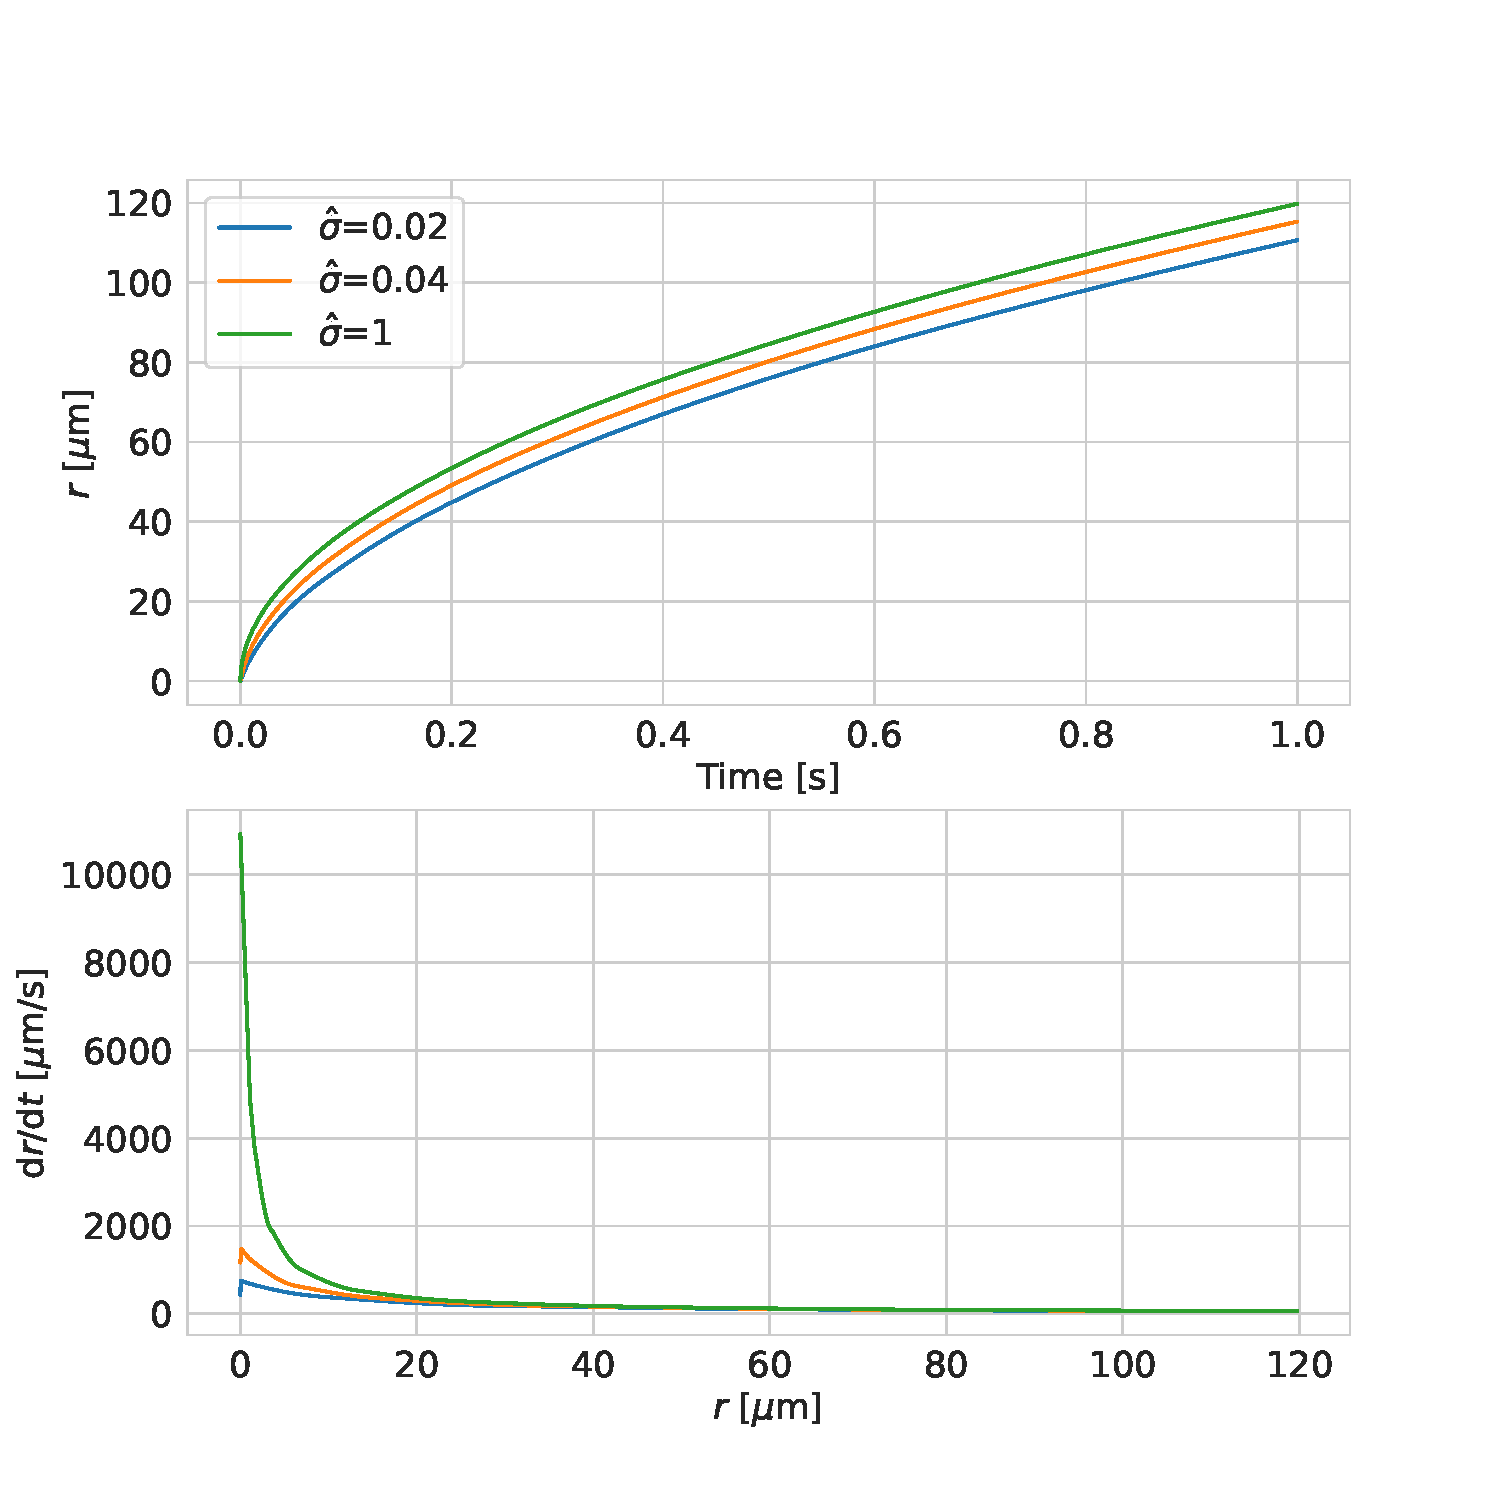
\includegraphics[trim={0 0 0 60},clip,width=1.0\textwidth]{Figures/dropwise_sigma_drdt.pdf}
    \caption{Dropwise condensation of a single droplet for different accommodation factors}
    \label{f:dropwise h_i}
\end{figure}
This behavior is attributed similarly to the interfacial heat resistance for a varying $\hat{\sigma}$; higher interfacial resistance (lower $\hat{\sigma}$) provides a longer growth delay. Nevertheless, after a certain period, the curves converge to reach linear steady growth. Nevertheless, this factor has proven to be detrimental to the wall heat flux calculation, due to the varying radius progression. This will be discussed further in Section \ref{s:future_work} 

As both the dropwise and Knudsen models replicate the expansion of a droplet in a vapor-only environment, it is valuable to examine the impact of temperature variation on these two models. It's crucial to note, however, that a significant distinction exists between these models beyond the surface presence. Specifically, the Knudsen model presupposes a uniform temperature within the droplet, whereas the dropwise model does not. Therefore, conclusive remarks cannot be made about their differences, as one is a product of thermodynamic principles while the other is essentially a heat transfer problem.
\begin{figure}[H]
    \centering
    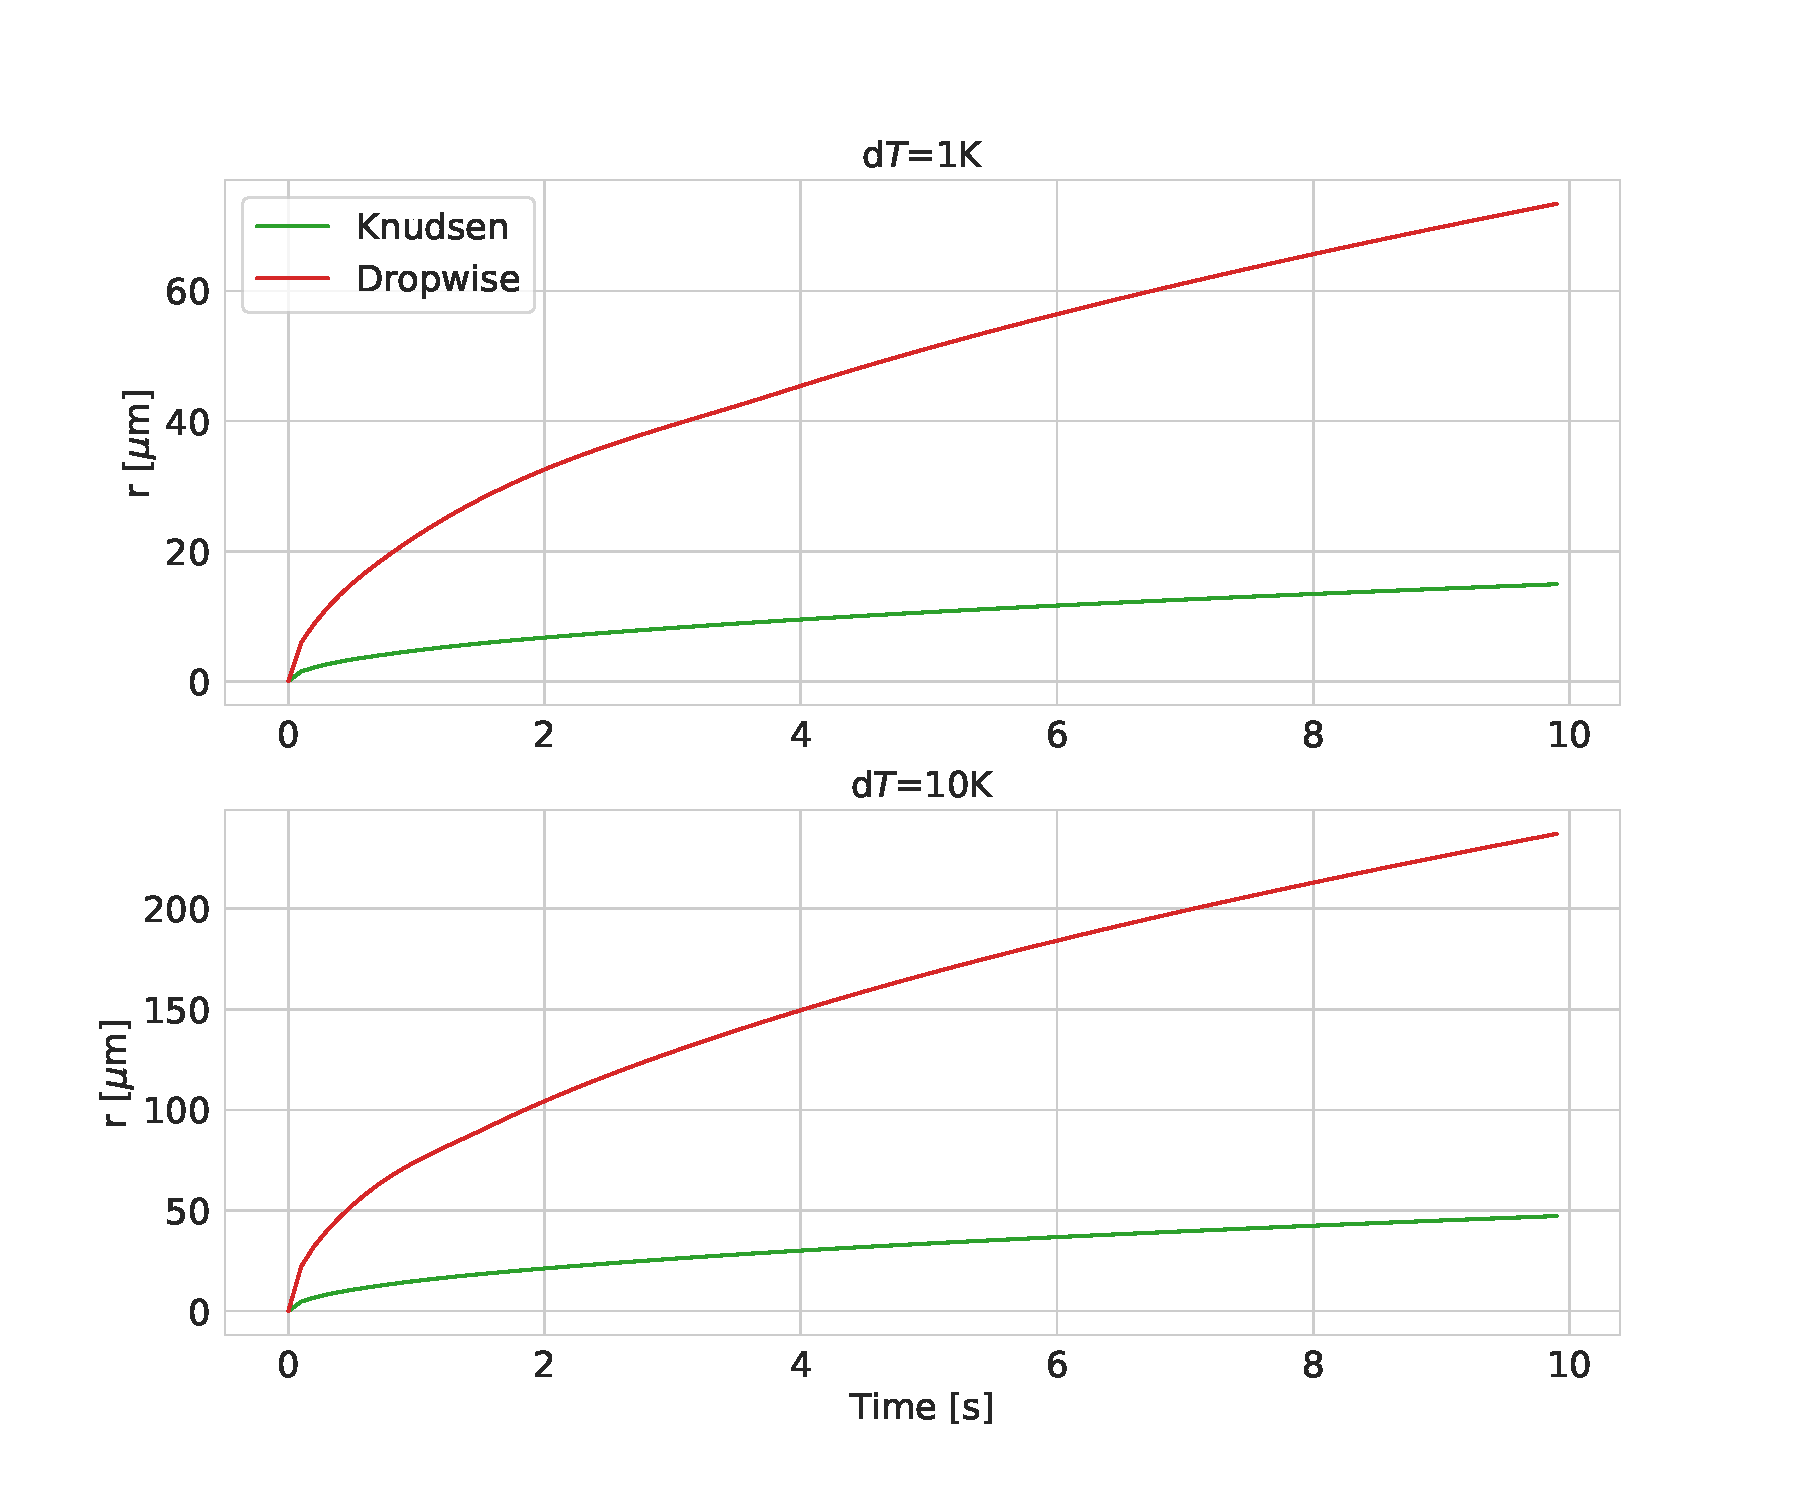
\includegraphics[trim={0 30 0 40},clip,width=1.0\textwidth]{Figures/r_knud_vs_dropwise.pdf}
    \caption{Dropwise condensation compared with the Knudsen model for two different temperature differences}
    \label{f:r_knud_vs_dropwise}
\end{figure}
The simulation configuration was established at an ambient temperature of $373\mathrm{K}$, with the dropwise model featuring a lower wall temperature and the Knudsen model having a higher droplet temperature. For the sake of demonstration, the radius is plotted in Figure \ref{f:r_knud_vs_dropwise} to feature its non-linearity when not squared.

Furthermore, the simulation was set up so that the initial droplet radius acquired from the dropwise model (Eq. \ref{eq:r_min_temp}) would serve as the initial radius for the Knudsen model. The contact angle was set to $\theta=175^\circ$ to acquire similar droplet volumes.

In comparison to the Knudsen model, it's evident that a droplet undergoing condensation on a surface is significantly more responsive to an increase in temperature differences. Within a span of $10\mathrm{s}$, the difference in the last recorded radii is about $50\mu\mathrm{m}$ and when increasing $\mathrm{d}T$, it increases to about $200\mu\mathrm{m}$. While both curves show similar growth progression with time, the gradients observed (especially for small droplets) for the surface case are much larger.
\begin{figure}[H]
    \centering
    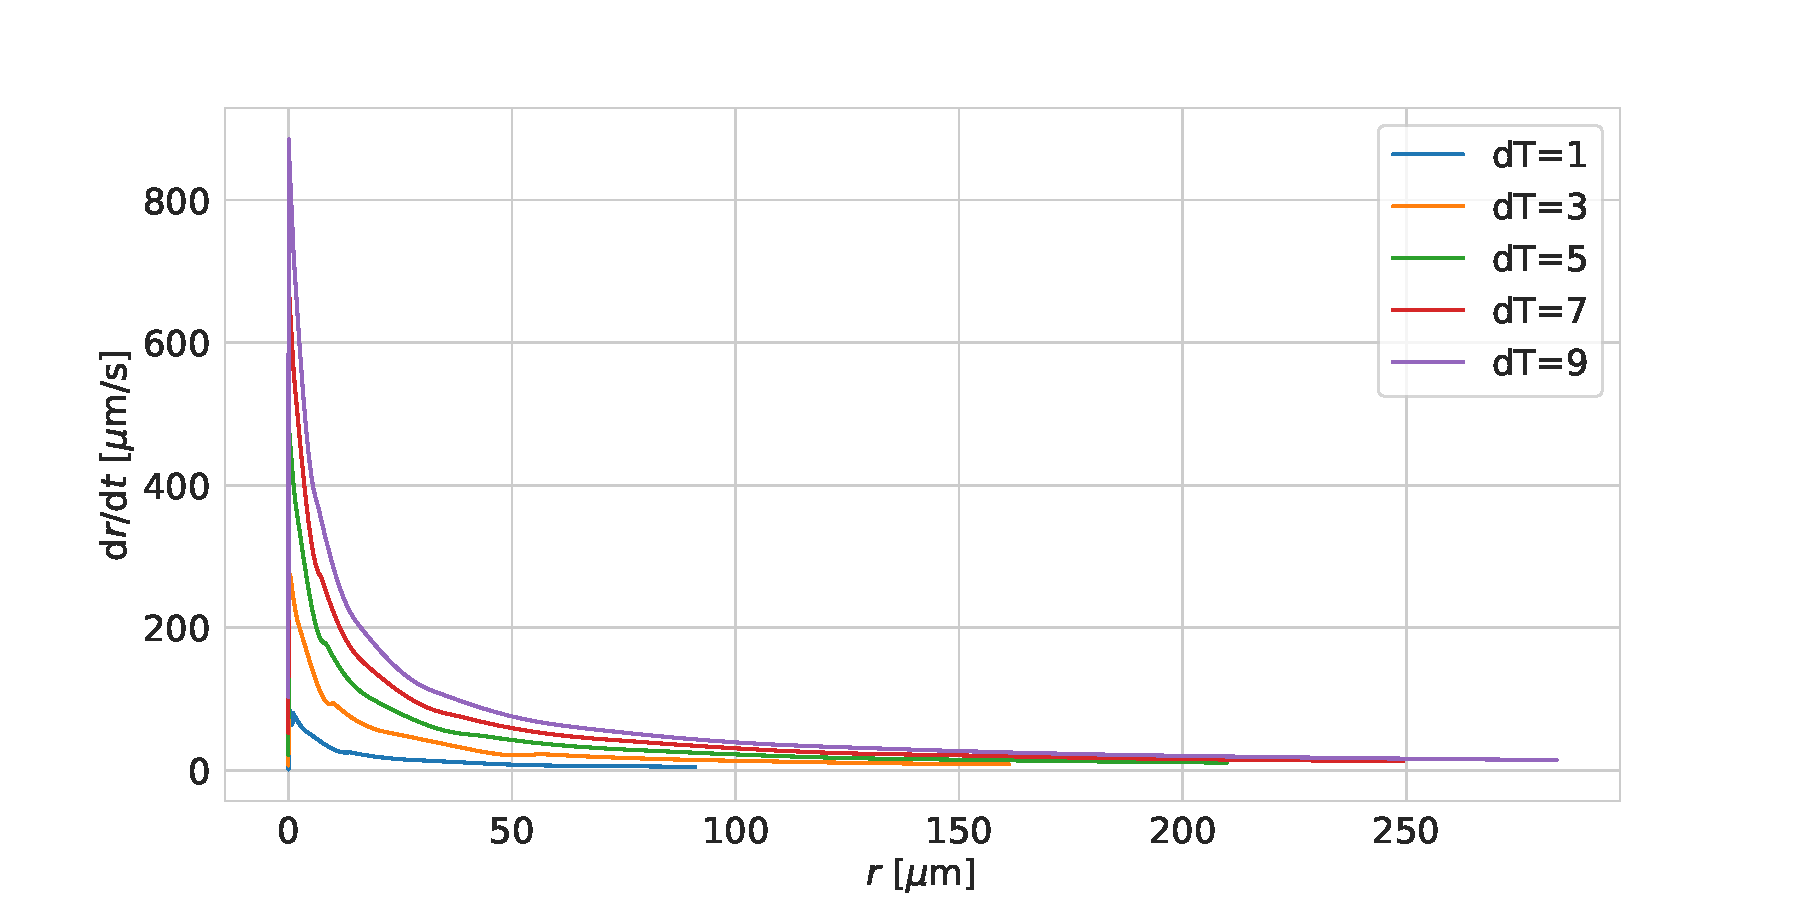
\includegraphics[trim={0 0 0 40},clip,width=1.0\textwidth]{Figures/drdt_const_assumption.pdf}
    \caption{Droplet growth rate for different wall temperatures}
    \label{f:drdt_het_constant}
\end{figure}
Lastly, the droplet growth rate is illustrated to assess the quality of the constant value assumption made in Section \ref{sss:Methodology-Heterogeneous-transport}. For this, the boundary conditions are fixed to values that will be comparable to data found in the literature. The saturation temperature is set to $T'=303\mathrm{K}$, which implies a saturation pressure of $p'=4.247\mathrm{kPa}$ and latent heat of $h_{vl}=2429\mathrm{kJ/kg}$. In addition, several wall temperatures are iterated through. The droplet growth rate is plotted against the droplet radius in Figure \ref{f:drdt_het_constant}.

An initial transient period can be observed for all $\mathrm{d}T$, where quick growth is observed for the freshly nucleated droplet. However, as $\mathrm{d}T$ increases, the amplitude of the growth rate changes significantly. After the initial period, the value can be seen as constant. It is thus anticipated, that the constant growth rate assumption might perform better for small wall-vapor temperature differences. Note that the simulation was fixed for $10\mathrm{s}$, therefore, the last value of $r$ will change, due to droplets reaching bigger sizes at higher $\mathrm{d}T$. It is also anticipated, that a larger maximal radius, dictated by the force balance, will provide better results under this assumption. This is due to the majority of the droplet's lifespan will be spent in this constant growth rate state.     
\subsection{Cylinder Case}\label{ss:Cylinder_case}
It is of interest to first inspect the influence of velocity on the supersaturation levels found in the classical cylinder flow. Because the supersaturation of the flow was artificially increased to provoke higher nucleation rates, the values are normalized by the maximal value of the reference case, $U=50\:\mathrm{m/s}$. This is demonstrated in Figure \ref{f:cylinder supersat}.
\begin{figure}[H]
    \centering
    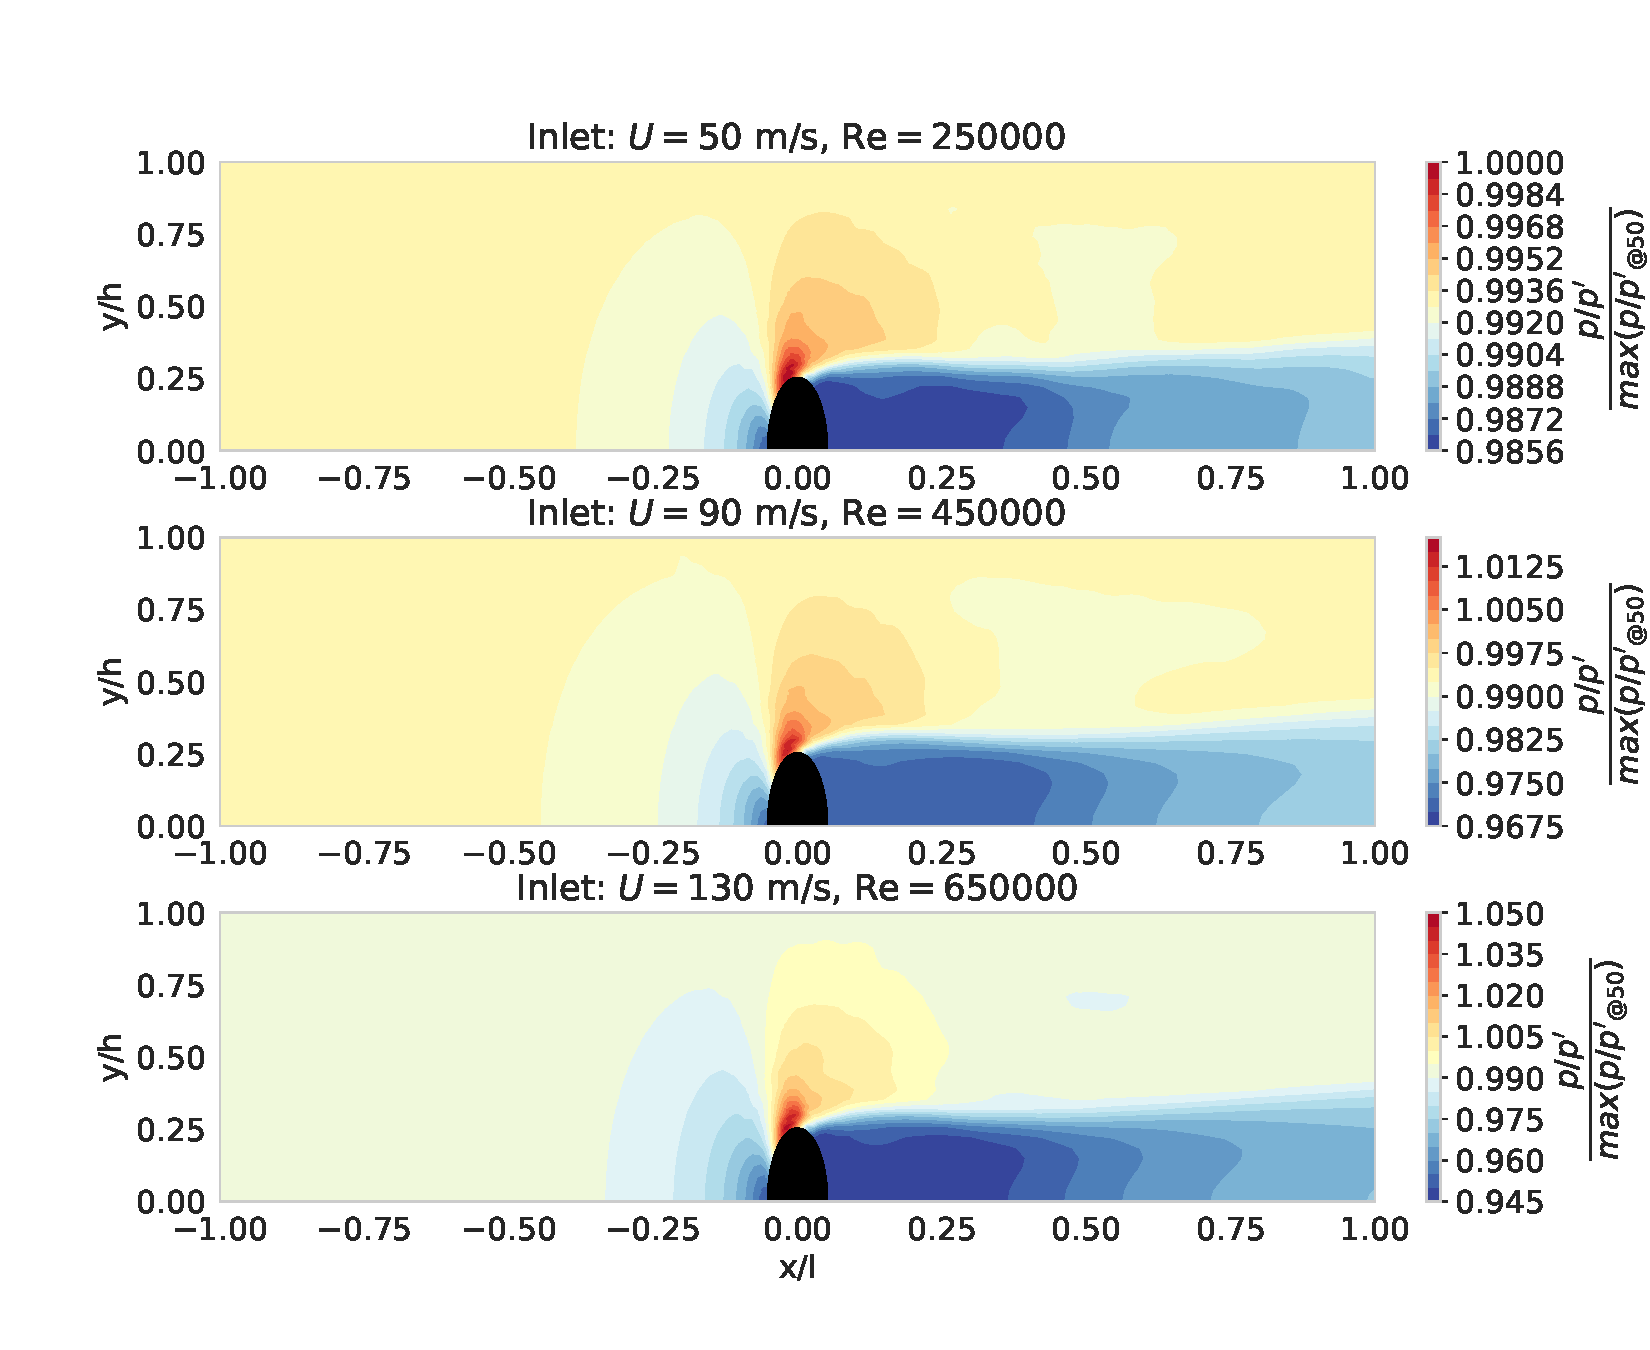
\includegraphics[trim={0 30 0 40},clip,width=1\textwidth]{Figures/supersat_plot_speed_compare.pdf}
    \caption{Supersaturation level in reference to the maximal value at $U=50$ $\mathrm{m/s}$}
    \label{f:cylinder supersat}
\end{figure}
It is noticeable that as the velocity rises, there is a rise of several percentage points in supersaturation levels. However, the pattern of the flow in relation to supersaturation remains consistent: the area beside the cylinder, where the maximum velocity is attained, results in the highest supersaturation. It can also be well observed that the supersaturation levels at the stagnation point and wake are relatively low. This strengthens the notion that the saturation pressure calculation is more sensitive to the temperature change than the local pressure change due to the change in velocity.
\begin{figure}[H]
    \centering
    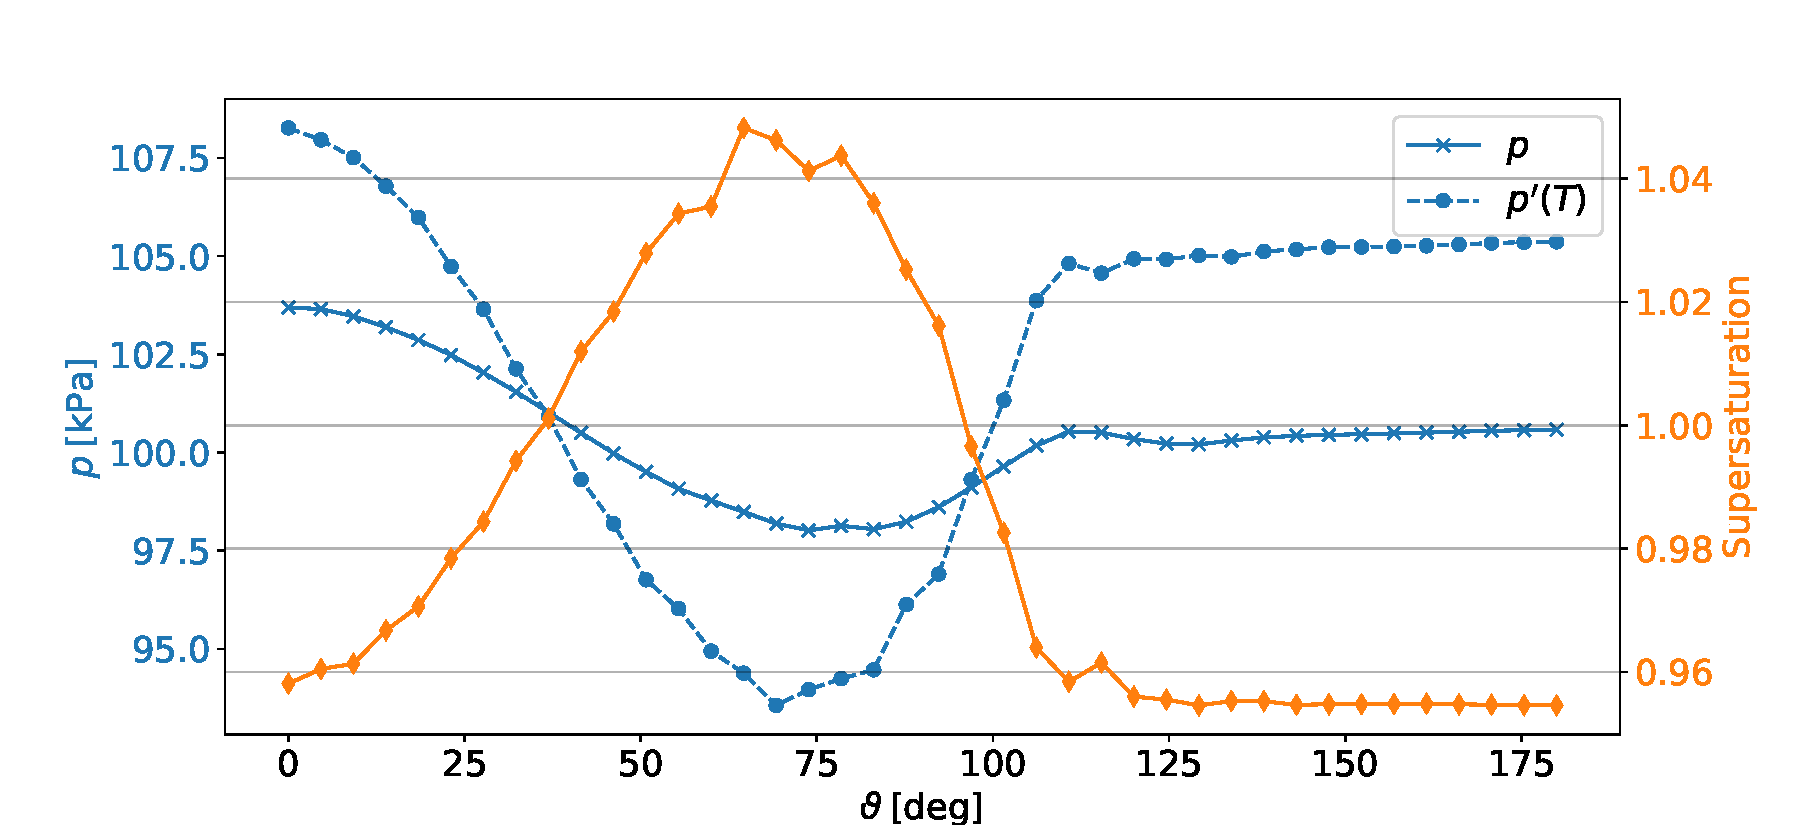
\includegraphics[trim={0 0 0 40},clip,width=1\textwidth]{Figures/supersat_angular.pdf}
    \caption{Acquired pressure values along the cylinder wall cells for $U=50$ $\mathrm{m/s}$ case.}
    \label{f:angular_supersat}
\end{figure}
These findings are further demonstrated in Figure \ref{f:angular_supersat}. Here, the calculated pressures and the corresponding supersaturation levels are plotted as a function of the angular coordinates around the cylinder, $\vartheta$, which varies between $0^\circ$ (stagnation point) and $180^\circ$ (wake center). This was done by acquiring the pressure and temperature values of the wall cells around the cylinder. The saturation pressure was then calculated using the temperature values with the Clausius-Clapeyron equation. The change in pressures can be easily followed: at the stagnation point, a higher pressure and temperature are observed as the flow is decelerated. Continuing around the cylinder body, the flow is accelerated and it can be observed that the saturation pressure drops quicker than the static pressure. The flow then reaches supersaturation conditions at the point where the two pressure curves cross. The flow is then again decelerated and detaches from the cylinder, which is depicted through the constant pressure observed at around $\vartheta=110^\circ$.
\begin{figure}[H]
    \centering
    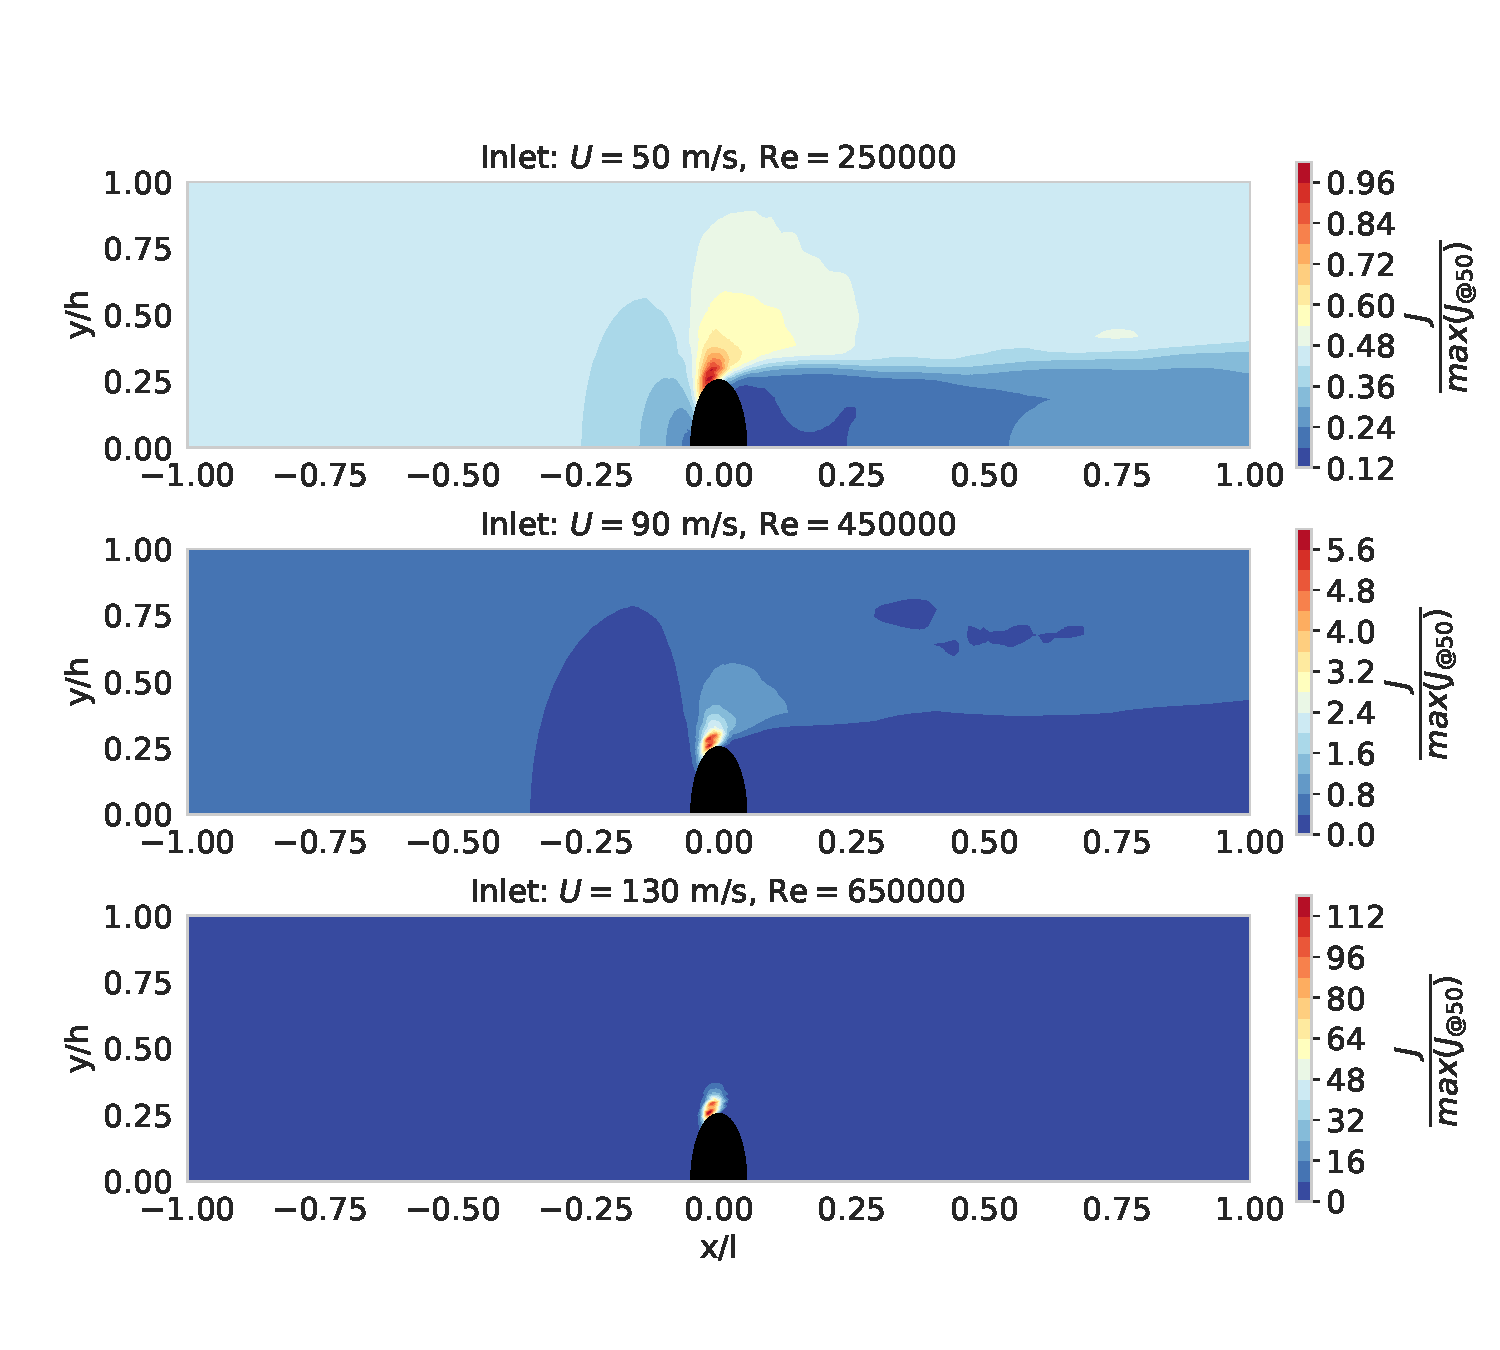
\includegraphics[trim={0 40 0 50},clip,width=1.0\textwidth]{Figures/I_plot_speed_compare.pdf}
    \caption{Nucleation rate in reference to the maximal value at $U=50\: \mathrm{m/s}$}
    \label{f:cylinder_nucleation}
\end{figure}
Although the change in supersaturation levels may seem small, Figure \ref{f:cylinder_nucleation} demonstrates that it has high significance concerning the nucleation rate. Similarly, the nucleation rate is normalized by the maximal value of the reference case. When almost doubling the inlet velocity, $J$ is increased more than fivefold. For the fastest inlet velocity case, the nucleation rate is more than a hundred times higher than the reference. This sensitivity to the supersaturation levels originates presumably from the exponential nature of the nucleation rate (Eq. \ref{eq:nucleation gerber}) and explains the need for further research for such occurrences in steam turbines. A small optimization of the turbine flow field can lead to a significant change in droplet formation rate. Although the results suggest that a hundred times more droplets are produced every second in the fastest velocity case, it is important to note that the flow is highly convective, resulting in the droplets being transported away from the vicinity of the cylinder quickly. In terms of droplet growth through the Knudsen model, it is difficult to conclude which source term influences the mass fraction $\alpha$ more significantly: higher droplet number due to higher nucleation, or lower droplet numbers but therefore more time is spent in the domain leading to more time for droplet growth.

Because the nucleation rate is not sufficiently high enough, $\alpha$ does not provide a wide enough range to acquire results capable of meaningful comparisons. These findings are consistent with ones found in literature, where nucleation rates reaching $10^{22}$ only result in $5\%$ of wetness fraction \cite{patel2016influence}. Moreover, due to evaporation observed in the wake, $\alpha$ may be further underestimated. The results for the droplets growth rate are presented in Appendix \ref{s:appendix A}. As the droplet temperatures were fixed at $373\mathrm{K}$, evaporation can take place if the vapor temperature exceeds this value. Thus, the wake acts as a source for $\alpha$. 
\begin{figure}[H]
    \centering
    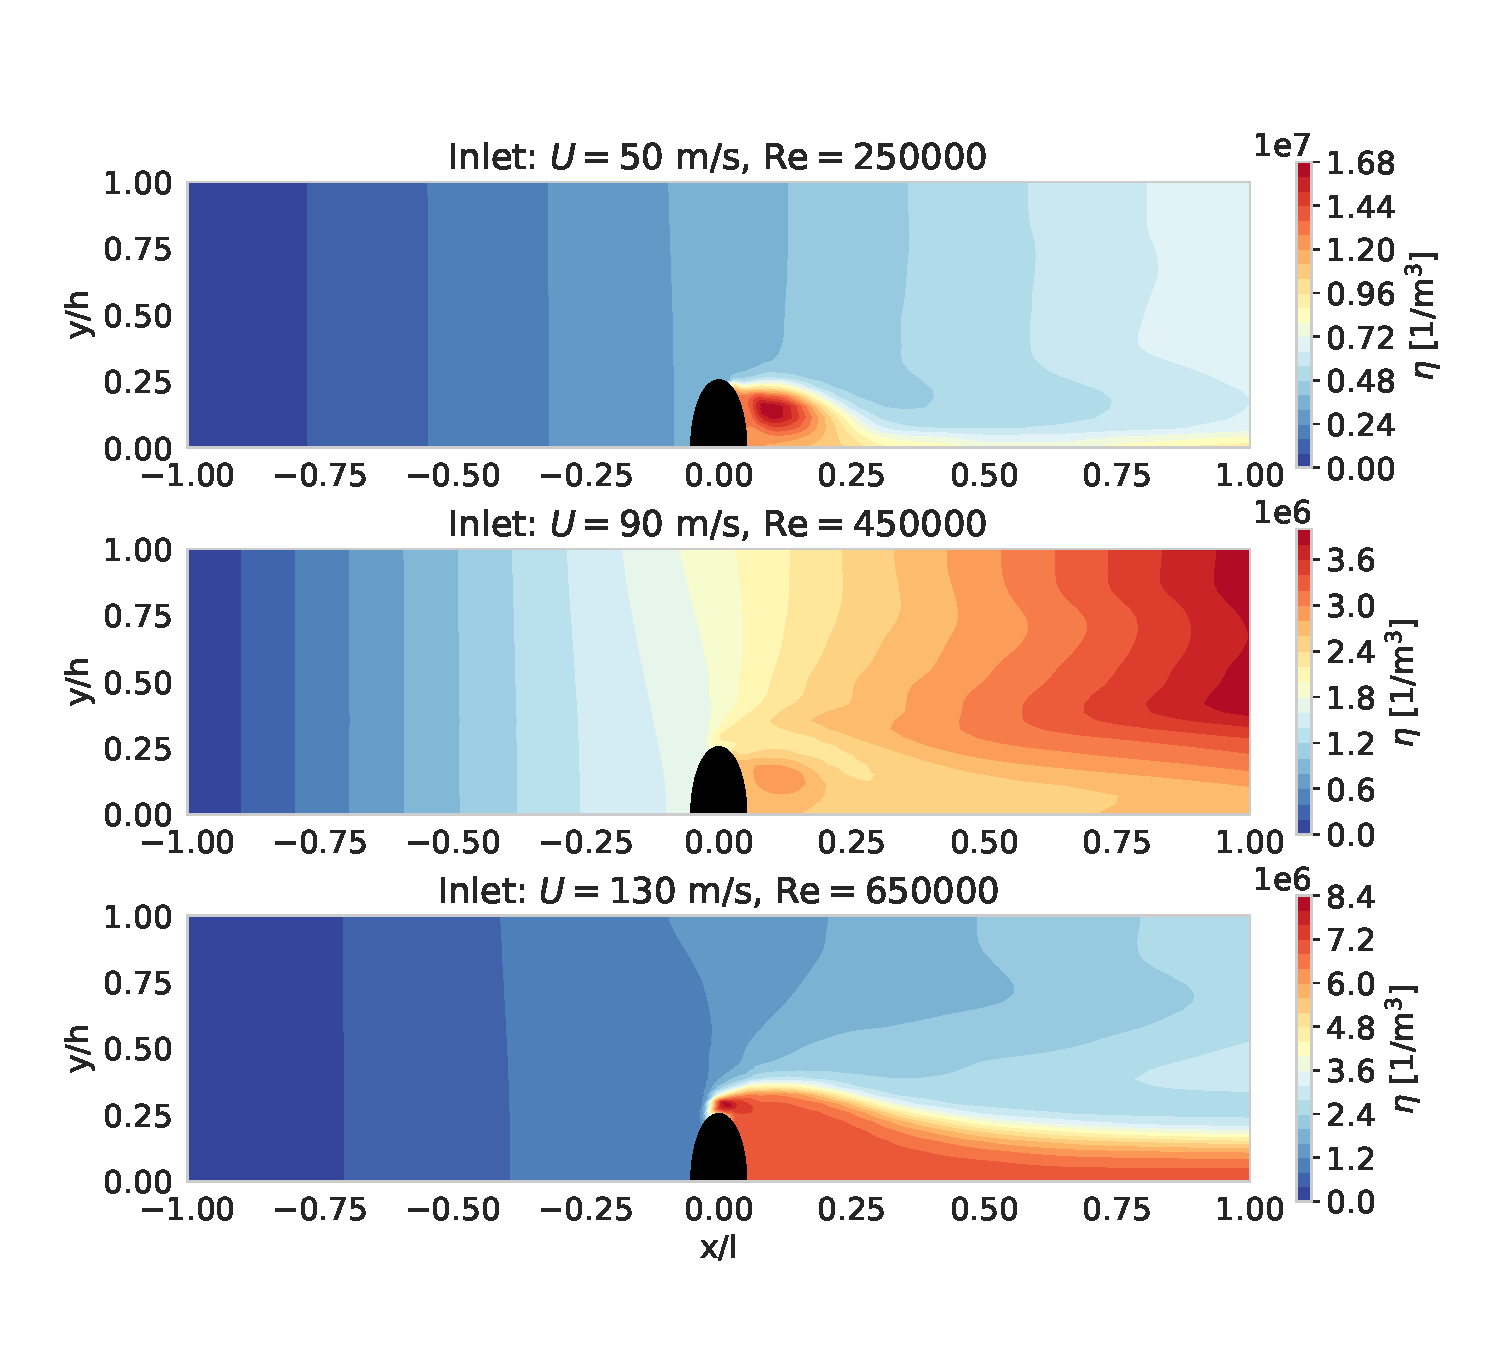
\includegraphics[trim={0 40 0 50},clip,width=1.0\textwidth]{Figures/N_plot_speed_compare.pdf}
    \caption{Droplet number per unit volume of vapor}
    \label{f:cylinder_dropletnum}
\end{figure}
The droplet number, $\eta$, can reveal some tendencies of the dispersed droplets within the domain. Figure \ref{f:cylinder_dropletnum} demonstrates the absolute $\eta$ for the three flow configurations. The distribution of droplets within the domain is very different for the three velocities. At $U=50\:\mathrm{m/s}$ and $U=130\:\mathrm{m/s}$ the droplets remain within the wake of the cylinder, while the wake of the higher velocity is significantly thicker up to the outlet. Although the nucleation rate is a hundred times higher for that case, it can be seen that the droplets are spread out more throughout the domain, presumably due to high convection. On the other hand, in the lower velocity configuration, it seems as if the droplets are "stuck" just behind the cylinder, which is supported by the droplet number in that region which is an order of magnitude higher than the two other cases. 

For $U=90\:\mathrm{m/s}$ a very different field is observed. Although some of the droplets remain within the wake, the majority escape it, dispersed within the flow far from the cylinder. The velocity profile and other transport quantities of this case do not reveal further information about these findings. It is therefore assumed that some interaction of the cylinder's boundary layer with the droplets causes them to escape the wake.

\subsection{Flat Plate Case}\label{ss:Dropwise_case}
For the calculation of the wall heat flux, the solution of $\bar{r}$ and $\mathrm{d}\bar{r}/\mathrm{d}t$ from the OpenFOAM solver will be first compared to that acquired from the Python RK45 method. For this, two meshes were utilized, where the one referred to as "High first cell" has a wall cell height of $400 \mathrm{mm}$ and the "Low first cell" has a height of $20 \mathrm{mm}$. For reference, the domain height is $10\mathrm{m}$. It was observed that refinement of the wall surface area does not influence the results. The results acquired for $\bar{r}$ are demonstrated in Figure \ref{f:r_hat_OF}. 
\begin{figure}[H]
    \centering
    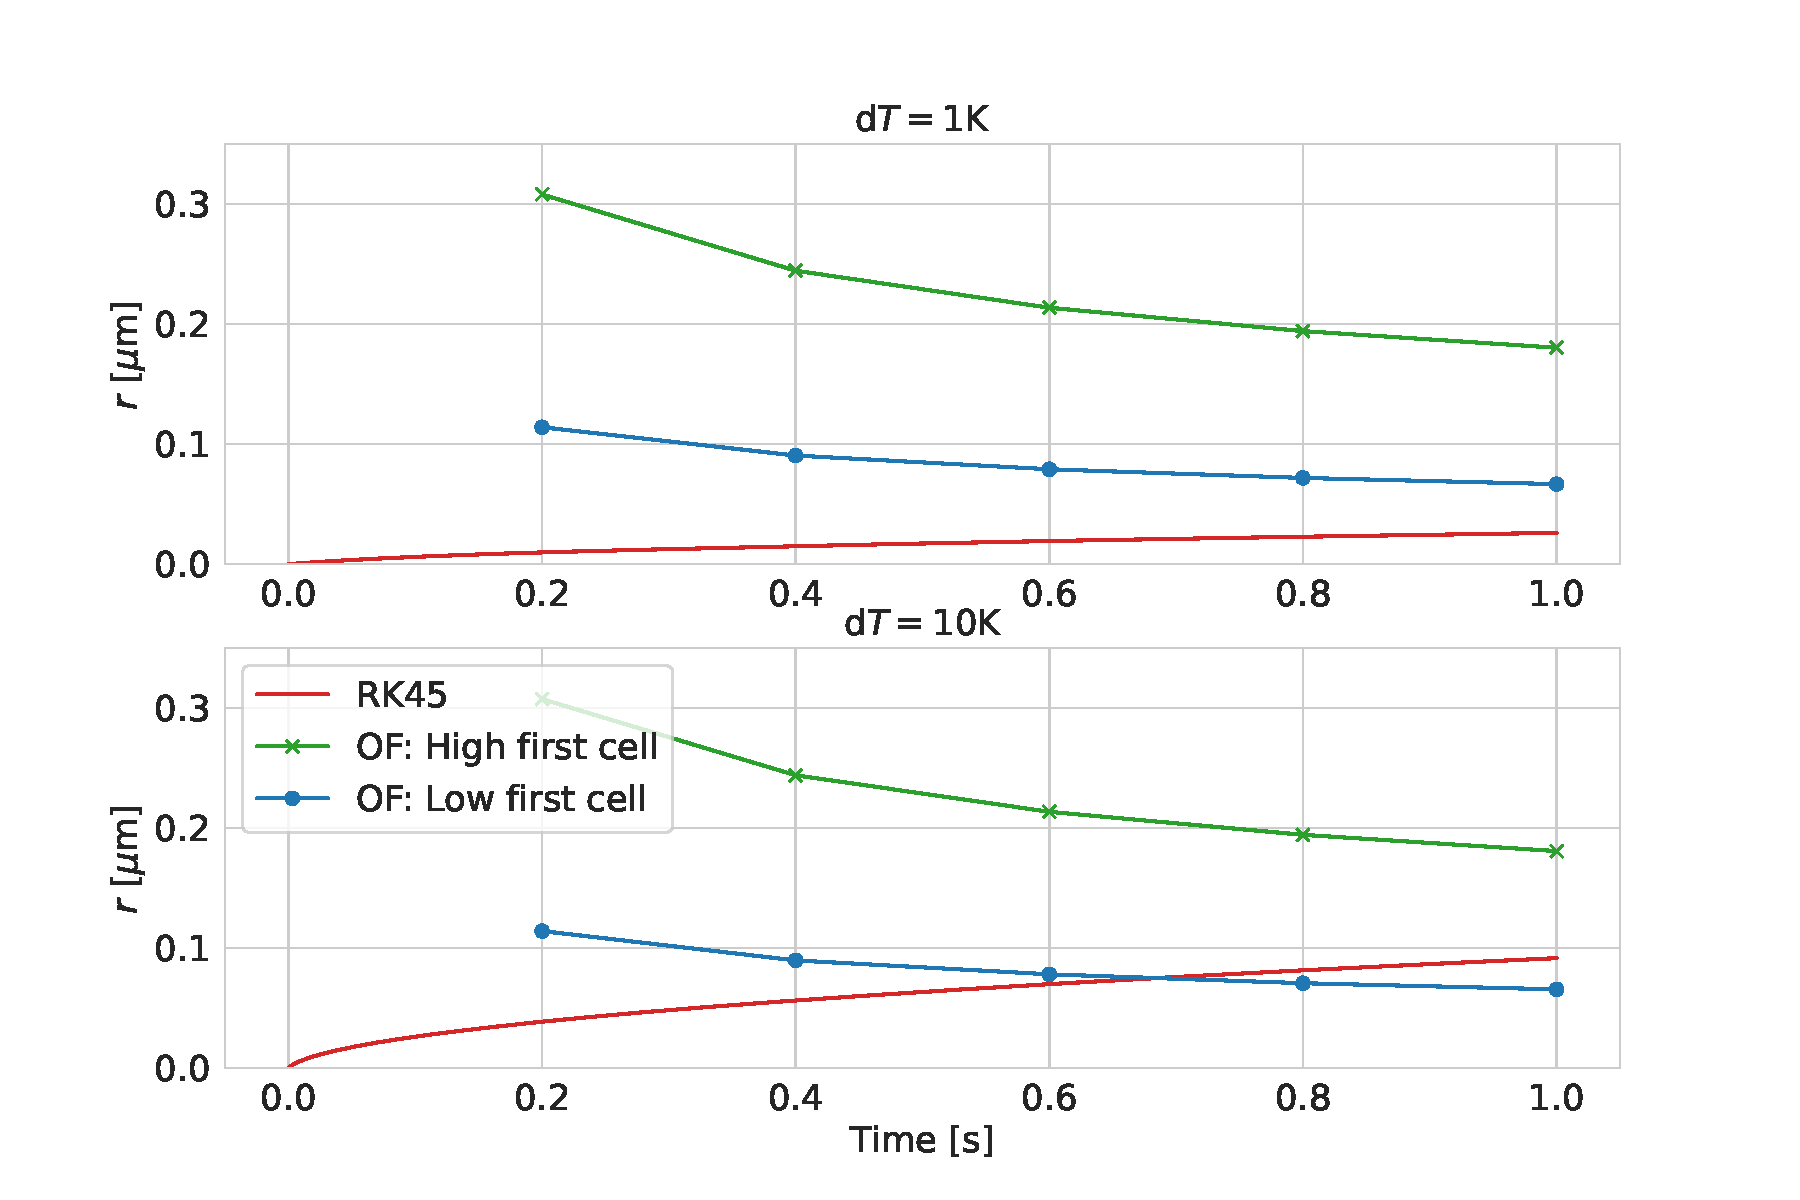
\includegraphics[trim={0 20 0 50},clip,width=1\textwidth]{Figures/r_bar_OF.pdf}
    \caption{Droplet radius progression with time. Comparison between RK45 solution and OpenFOAM simulations for two cell refinements.}
    \label{f:r_hat_OF}
\end{figure}
It can be directly observed that the height of the first cell has a significant influence on the acquired results. Furthermore, the sensitivity of the OpenFOAM solution to a varying $\mathrm{d}T$ is extremely minimal. For the "Low first cell" solution, the end value would be overestimated for $\mathrm{d}T=1\mathrm{K}$ and underestimated for $\mathrm{d}T=10\mathrm{K}$. It can also be observed that $\bar{r}$ starts from a higher value and then decreases. This is possibly due to $\eta$ increasing rapidly as the nucleation process continues with each timestep, while $\alpha$ only decreases marginally. The progression of the mass fraction with time is illustrated in Appendix \ref{s:appendix A} Figure \ref{f:Mass_Fraction_het}.
\begin{figure}[H]
    \centering
    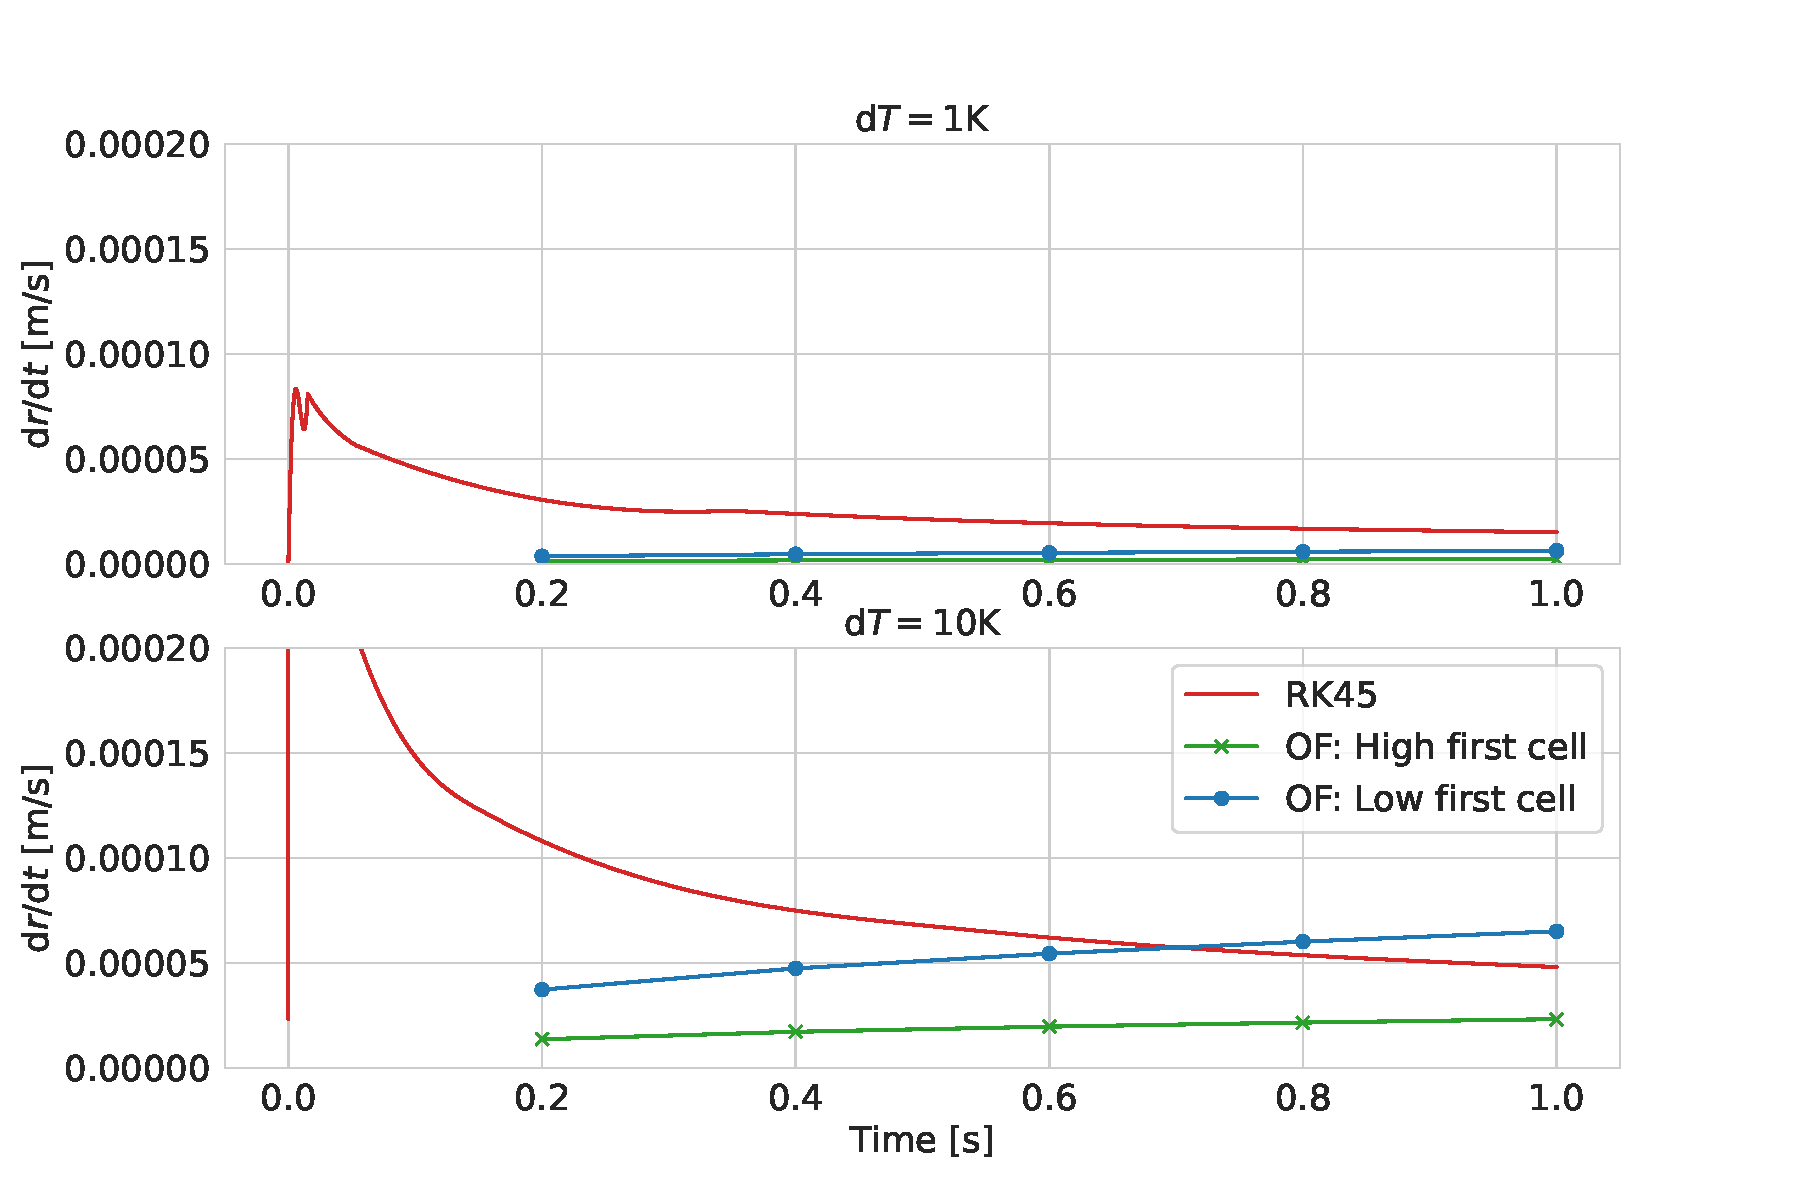
\includegraphics[trim={0 20 0 50},clip,width=1\textwidth]{Figures/drdt_OF.pdf}
    \caption{Droplet growth rate progression with time. Comparison between RK45 solution and OpenFOAM simulations for two cell refinements.}
    \label{f:drdt_OF}
\end{figure}
The droplet growth rate calculated in OpenFOAM is however much more sensitive to $\mathrm{d}T$, presumably due to being a direct function of it. This is illustrated in Figure \ref{f:drdt_OF}. Here, both meshes underestimate $\mathrm{d}\bar{r}/\mathrm{d}t$ for the lower $\mathrm{d}T$ while for the higher one, the finer mesh case almost manages to acquire a similar solution as the RK45 solver. This result has big significance on the calculation of the wall heat flux as it is a direct function of $\mathrm{d}\bar{r}/\mathrm{d}t$. Nevertheless, the initial transient period is not reproduced by the OpenFOAM solver and will therefore lead to a higher average error. 

It should be noted that the temperature values at the first cell acquire a value lower than the wall boundary condition. The reason for this and its potential to influence the aforementioned variables will be discussed in Section \ref{s:future_work}. 
\begin{figure}[H]
    \centering
    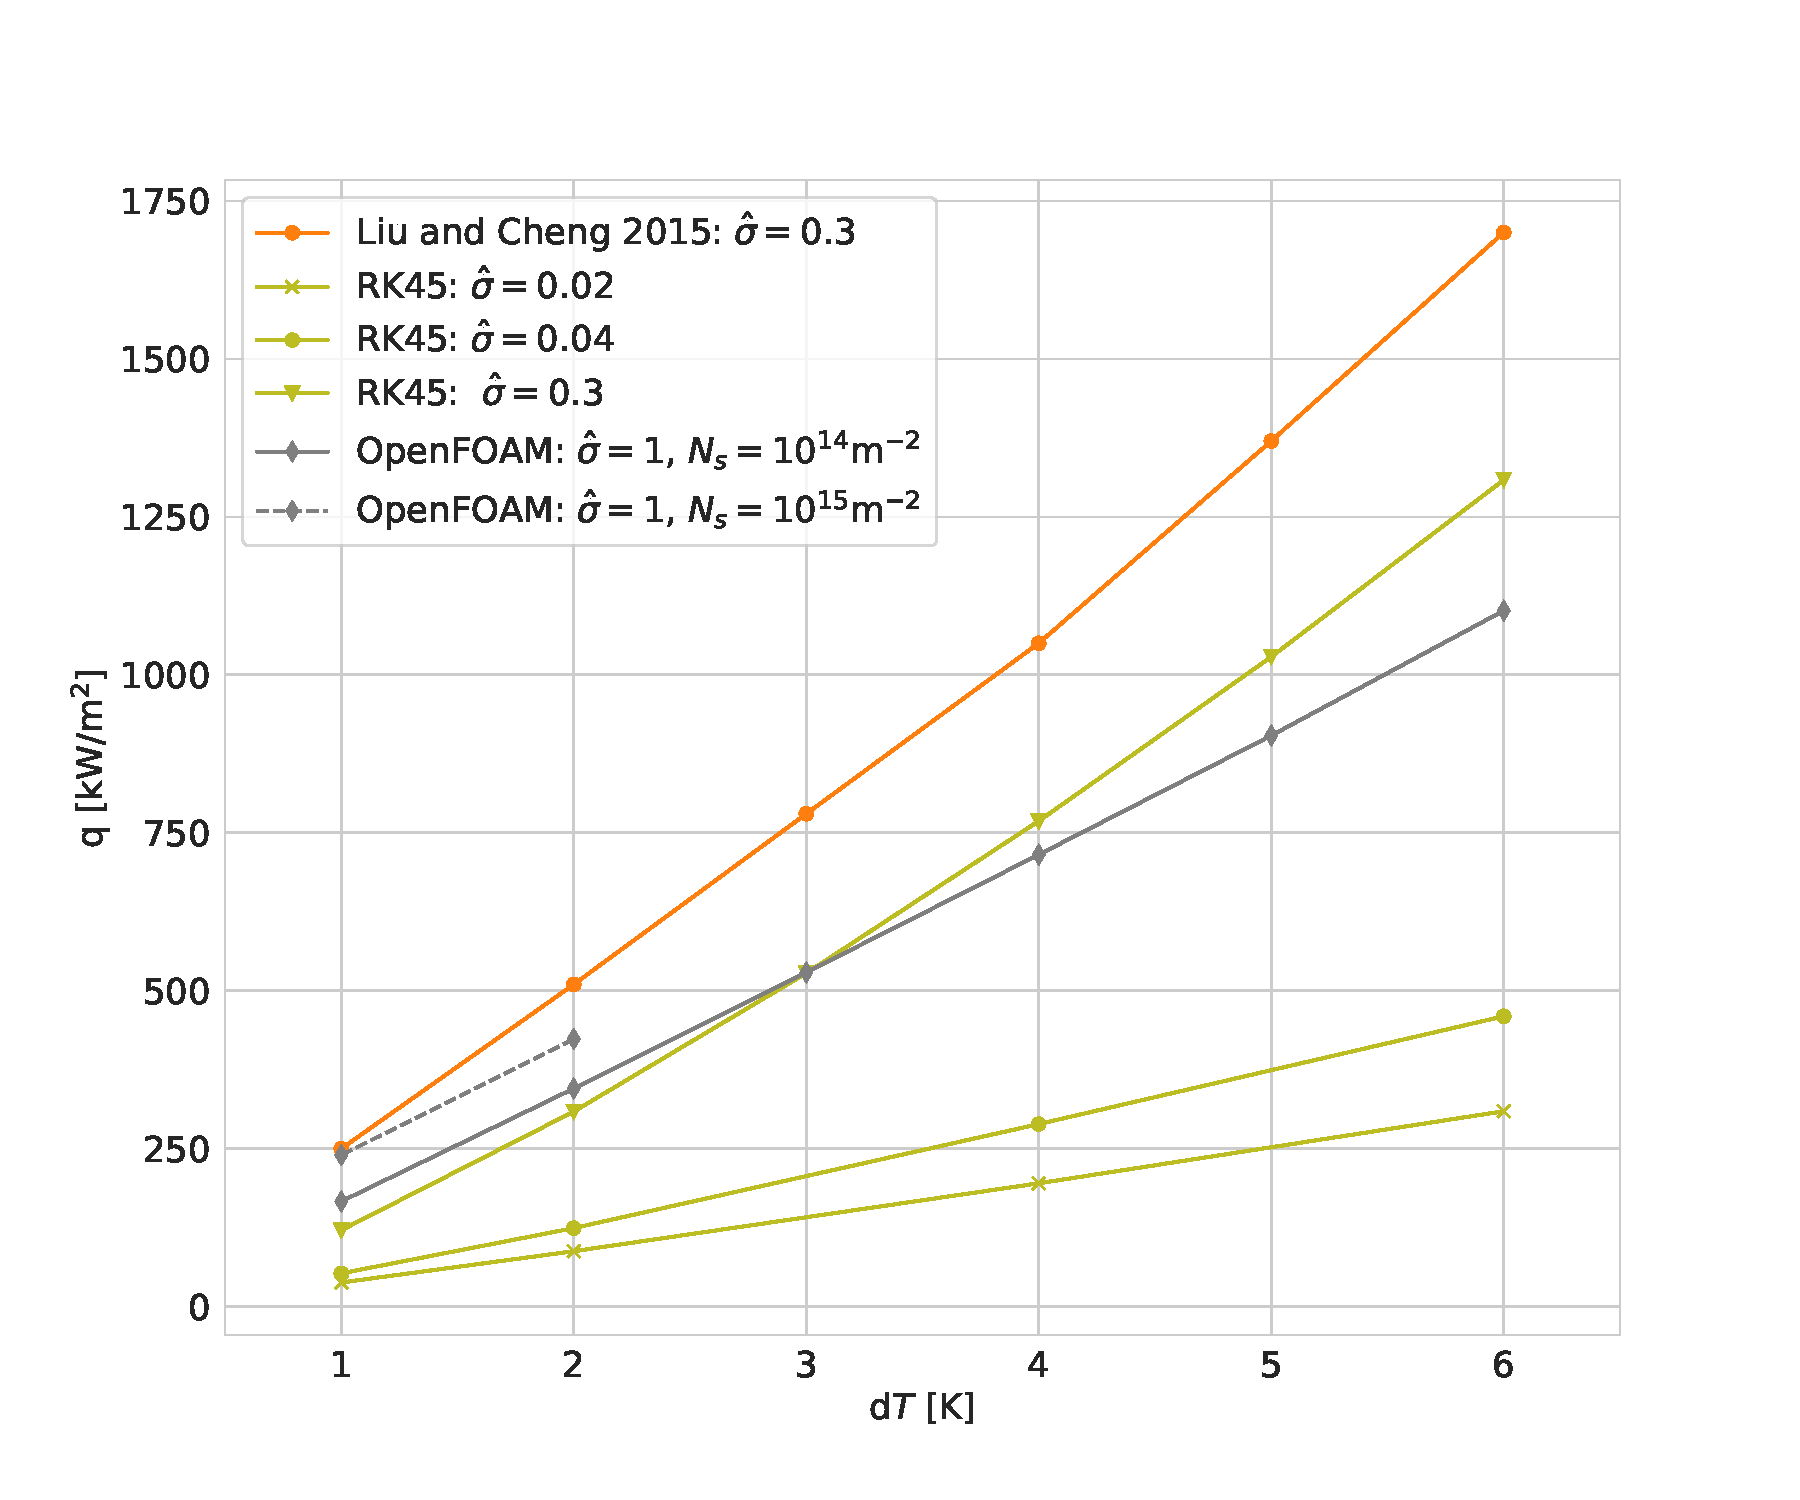
\includegraphics[trim={0 20 0 70},clip,width=1\textwidth]{Figures/heatflux_compare.pdf}
    \caption{Wall heat flux values for increasing saturation-wall temperature differences at a constant vapor temperature of $T'=373\mathrm{K}$. Results are compared with the work of Liu and Cheng \cite{liu2015dropwise2}.}
    \label{f:heat_flux_compare}
\end{figure}
The wall heat flux as a function of the wall-vapor temperature difference is presented in Figure \ref{f:heat_flux_compare}. Results acquired from the RK45 method and OpenFOAM solver are compared with values found in the literature and several critical values were iterated through (see legend). As mentioned before, the droplet size distribution models used in this work are different to the compared data: Liu and Cheng \cite{liu2015dropwise} have utilized an additional model for very small droplets while using the Le Fevre and Rose model \cite{le1966theory} for droplets bigger than a few microns. The saturation temperature investigated is $373\mathrm{K}$. Pressure and latent heat were selected accordingly. Lastly, it should be mentioned that the maximal droplet radius calculated under these conditions is approximately $r_{max}\approx 3\mathrm{mm}$.

The RK45 solution shows a great amount of dependency on the accommodation coefficient $\hat{\sigma}$. As seen in Figure \ref{f:dropwise h_i}, $\hat{\sigma}$ influences mostly the initial transient period. When integrating the product of heat flow and droplet population with respect to the radius, it is expected that different growth progression will have implications for the heat transfer, thus resulting in different heat flux to the wall. Liu and Cheng provided a value for the accommodation coefficient of $\hat{\sigma}= 0.3$ but only provided a range for the nucleation density $N_{s}$. Two values were therefore assessed. 

The OpenFOAM solver does not react significantly to $\hat{\sigma}$ and aligns well for the lower $\mathrm{d}T$ with the RK45 solution. Moreover, for both cases, its slope is consistently lower than that of the RK45. This originates presumably from the constant droplet growth rate assumption which breaks down at higher $\mathrm{d}T$. At $N_{s}=10^{15}\mathrm{m}^{-2}$, the solution is shifted upwards, retaining the slope of the other solution. Higher $\mathrm{d}T$ values for this case were not acquired, due to the temperature of the first cell acquiring unphysical temperatures.

Although both solvers do not recreate the values found in the literature with high accuracy for a recommended $\hat{\sigma}$, the trend of the curves can be well observed. A good agreement can be found with values provided by Liu and Cheng \cite{liu2015dropwise} where given constants allowed an accurate recreation of the case. In their proposed model, very small droplets acquire a different droplet population model. Furthermore, their model takes into account the observation, that droplet growth at those sizes is purely driven by condensation and not by coalescence, a property that Le Fevre and Rose assumed is similar to all droplet sizes. It is thus assumed, that further implementation of more accurate population models may yield even better results than those presented in this study.  
\newpage
\section{Discussion and Future Work}\label{s:future_work}
\subsection{Droplet Growth}
The Knudsen and dropwise condensation models directly adapted from the literature have been used as helpful tools for two applications
\begin{enumerate}
    \item Provide a reference for the derived $d^{2}$ growth model.
    \item Provide qualitative information on their properties for the development of the OpenFOAM solver.
\end{enumerate}

Concerning the first point, it was observed that the implementation of the "infinite conductivity" model in the code leads to similar properties such as the Knudsen model. When increasing $\mathrm{d}T$, the $d^{2}$-law scaled proportionally as the Knudsen model. Furthermore, it was shown that the implementation of the Kelvin equation for the calculation of the supersaturation level of the ambient mass fraction would deliver comparable conditions as the supersaturation level of vapor in a pure domain. On the other hand, removing the infinite conductivity term in the $d^{2}$ code has provided significantly different results which did not scale accordingly with $\mathrm{d}T$. 

It is thus to be answered if removing the infinite conductivity term would be appropriate for air-vapor mixtures when potentially implementing such a model in a CFD code. Nevertheless, results show that it is feasible to implement such a model for droplet growth in multi-species CFD simulations. Difficulties may arise when for example implementing the $d^{2}$ model with the infinite conductivity term in an Eulerian/Eulerian code due to the iterative nature of the calculation: solving the ODE using $\bar{r}$ would presumably lead to inaccurate mass growth rates, leading to inaccurate heat flux out of the droplet and thus leading to false droplet temperatures. Therefore, an approach to determine the temperature using capillarity effects proposed by Gyarmathy \cite{gyarmathy1962grundlagen} could be appropriate. Such an approach would suggest that the droplet temperature could be calculated using field variables such as the saturation temperature, the temperature of the gas, the critical radius and the average radius. For future work, it would be appropriate to assess the quality of the results using such an approach compared with the infinite conductivity term.

The dropwise model for heterogeneous condensation provided droplet growth results that agree well with data presented by Marengo \cite{marengo2022surface}. Furthermore, the model has shown that considering the growth rate as constant for low $\mathrm{d}T$ could be a strong assumption. However, this must be further investigated for different saturation conditions, thermal conductivities, accommodation coefficients etc. Thus, it can't be concluded that such an assumption holds under all conditions. It is therefore suggested that further investigation concerning this assumption is needed for further utilization of the model in an Eulerian/Eulerian code.

Lastly, although the radius does converge to the same value, its dependence on the accommodation coefficient proves that it may need tuning for different scenarios to fit experimental data. This difficulty in the selection of an appropriate accommodation factor is the reason why the Knudsen model was developed by Gyarmathy \cite{gyarmathy1962grundlagen}. Utilizing the Knudsen number to model the convection coefficient may prove to be beneficial in the heterogeneous case as well and thus provide a more robust model. Perhaps, tuning the empirical factor in the Knudsen model may prove to be sufficient for an increase in model accuracy. 
\subsection{Homogeneous Condensation}
The Eulerian/Eulerian model, thoroughly presented by Gerber and Kermani \cite{gerber2004pressure}, for the simulation of non-equilibrium condensation within steam turbines proved to be a simple and ready-to-use approach. Although non-equilibrium conditions were artificially imposed, the results provided have shown qualitatively physical properties. An exception is the droplet number for the case of $U=90\:\mathrm{m/s}$ where it was observed that the majority of the droplets escaped the wake of the cylinder. The reason behind this behavior is yet to be discovered. However, variables such as the turbulent kinetic energy and dissipation rate have revealed that they are consistent with the other cases and show physical characteristics in general. Therefore, further investigation of this case must be conducted.

The sensitivity of the nucleation rate to the velocity has provided further insight into the importance of accurate modeling of such flows in turbines. With high non-equilibrium conditions due to the presence of shock waves, turbulence and other complex flow characteristics, it is clear that a strong engineering tool such as an Eulerian/Eulerian code can assist when making design choices and thus potentially reduce the nucleation rates by marginally reducing the supersaturation levels. 

If the manufacturing of a turbojet engine with a hydrogen combustor is feasible within the near future, the Eulerian/Eulerian formulation for pure vapor will need to undergo further modifications, such as introducing additional species conservation equations, besides the replacement of the Knudsen with the $d^{2}$ condensation model.   
\subsection{Heterogeneous Condensation}
It was firstly assessed, whether the principles of the Eulerian/Eulerian code manage to reproduce the behavior of the droplet radius and its growth rate. Changes consisted of a correction term to the calculation of the average radius, and the nucleation of the droplets was distributed over each time step. It was observed that the average radius calculated with the solver had two significant characteristics: a) highly insensitive to $\mathrm{d}T$, and b) highly sensitive to the first cell height. Concerning the first point, it is clear that the droplet number (used for the calculation of the average radius) is only dependent on the nucleation rate. Hence, if the number of droplets per surface area is fixed, as done by the reference study \cite{liu2015dropwise}, $\mathrm{d}T$ can't influence the average radius. Therefore, the mass fraction and the density of the vapor remain the only field variables that influence the radius. It is therefore clear why the average radius must decrease with each time step; as the nucleation proceeds, the mass fraction will decrease accordingly, the droplet number will increase, and a reduction in the average radius will be observed. Its high dependence on the mesh originates from the calculation of the nucleation rate (Eq. \ref{eq:sim_nucleation_process}). The proportion of wall cell surface area to wall cell volume results in the nucleation site density, $N_{s}$, being effectively divided by the height of the cell. Thus, the lower the cell, the higher the nucleation rate, which therefore leads to a lower average radius. This problem arises due to the quiescent nature of the simulation, where droplet clearance out of the domain through sweeping or convection is not accounted for. It comes therefore into question if a modification to the nucleation rate source term is needed or alternatively find a correlation that will allow clever decision-making of the wall cell height. Despite its inaccuracy, the droplet growth rate and thus the wall heat flux still manage to reproduce the expected trends.

This notion is further supported by the findings concerning the unphysical temperatures found in the wall cells. The strength of the source term in the energy conservation equations is clearly too high. Due to the aforementioned reasoning, the high increase in the droplet number will result in a rapid increase of $S_{d}$, which will in turn act as an unphysical sink. If convection was introduced, this would presumably also influence the velocity field accordingly. This reinforces the argument that additional evaluation of nucleation rate calculations is necessary when dealing with heterogeneous scenarios. Lastly, it is suspected that its influence on the vapor density and thus other calculated variables could provide a significant error in the results due to the range of unphysical temperatures observed.

The growth rate sensitivity to $\mathrm{d}T$ was expected, as it is a direct function of this difference. Furthermore, it was observed that the refinement of the mesh resulted in less deviation throughout the simulation. This is detrimental to the calculation of the heat flux as it is the only term in the derived analytical solution (Eq. \ref{eq:wall_heat_flux_analytical}) which is acquired through the Eulerian/Eulerian principles. However, this approximation works well after the initial transient period is over, and the solution converges to a constant growth rate. Considering a superhydrophobic surface (very large contact angles) would suggest that the total time the droplet spent on the surface before falling off due to gravity would decrease drastically as $r_{max}$ would decrease. This is because the total surface area for adhesion between the liquid and the substrate would decrease with increasing contact angle. As a result, the initial transient period would increase in significance due to the short droplet lifespan. The assumption of a constant droplet growth rate will presumably fail under such circumstances. The question is therefore raised concerning an alternative treatment of the droplet growth rate if such conditions are met. Under the conditions simulated for this study, a relatively high maximal radius was acquired ($r_{max}\approx 3\mathrm{mm}$). Because of the extended duration of growth linked to this value, the reasonable alignment of the solvers with the literature data can be partially attributed to the prolonged constant growth period, thus a relative weakening of the initial transient period.

For the calculation of the wall heat flux, two clear trends were observed for the RK45 solution: 
\begin{enumerate}
    \item For low $\mathrm{d}T$, wall heat flux values have the smallest deviation from literature values and the OpenFOAM simulation.
    \item A change of $\hat{\sigma}$ provides an offset to the curve and a large change of the slope.
\end{enumerate}
Concerning the first point, the small deviation from the OpenFOAM simulation originates from the constant radius growth rate assumption, which proves to hold under these conditions. Then, as $\mathrm{d}T$ increases, the solutions diverge presumably due to the difference between the analytical, simplified integration, and the trapezoidal method used for the RK45 solution. 
The departure from the values presented in the literature is likely due to variations in droplet population models, a topic that will be addressed shortly.

The results presented in Figure \ref{f:dropwise h_i}, illustrating the droplet radius progression with time, and the growth rate as a function of $r$ for different $\hat{\sigma}$ hold great significance for the calculation of $q$. For droplets smaller than $20\mu m$, there is a very large deviation in the growth rate. This can be explained by considering the resistances throughout the droplet for the calculation of the heat transfer. The small size of the droplet leads to the strengthening of the convective heat transfer component in comparison to the conduction through the droplet. After the droplet has reached a certain size, conductive resistance gains significance, and thus the droplet growth rate sinks. It is clear that if $h_{i}$ varies in orders of magnitude due to a change of $\hat{\sigma}$, the initial period will be affected drastically. Integration of the growth rate with respect to $r$ will therefore lead to very different wall heat flux, as the integration boundaries remain independent of these variables. 

Liu and Cheng \cite{liu2015dropwise} provided a detailed demonstration of their population model and validated their model against experimental data from different studies. For the calculation of the wall heat flux, they used the following calculation
\begin{equation}
    q=\int_{r_{min}}^{r_{eq}}n(r)Q_{d}\mathrm{d}r+\int_{r_{eq}}^{r_{max}}N(r)Q_{d}\mathrm{d}r
\end{equation}
where $n(r)$ is the population model for droplets of very small size, and $r_{e}$ is the equivalent radius, also referred to as the coalescence radius. In other words, $n(r)$ is used for droplets of the size that their growth through coalescence is highly unlikely \cite{marengo2022surface}. They found that $N(r)$, proposed by Le Fevre and Rose \cite{rose1976further}, works well for larger droplets, where growth can also occur through coalescence. $n(r)$, proposed by Wen and Maa \cite{WEN1976225}, is a model which unlike the work of Le Fevre and Rose was not developed empirically, but rather using population balance models, which originate from theories that describe the evolution of particle population. 
\begin{figure}
    \centering
    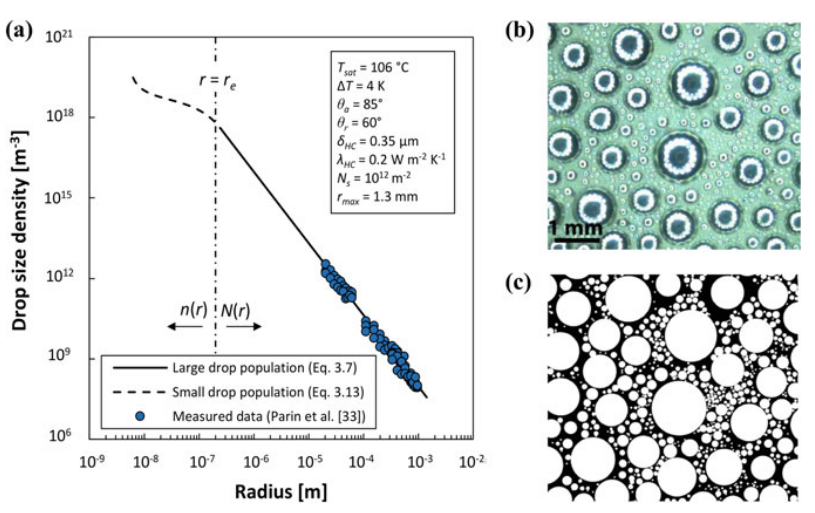
\includegraphics[trim={0 0 0 0},clip,width=1\textwidth]{Figures/Parin_exp.png}
    \caption{Results presented by Marengo \cite{marengo2022surface} of an experimental study conducted by Parin et al. \cite{PARIN2020115718}. a) Drop size density (population model) of droplets counted vs. the radius of the droplets observed. b) and c) are images acquired from the high-speed camera used in the experiment for the counting.}
    \label{f:parin}
\end{figure}

Figure \ref{f:parin} presents experimental results provided by Parin et al. \cite{PARIN2020115718}, where droplets of different sizes were counted using image processing techniques and compared to the population models. It can be seen that the usage of $N(r)$ between $r_{min}-r_{max}$, as implemented in OpenFOAM for this study, will result in an overestimation of the population of these very small droplets under these conditions (see legend). The trend of underestimating the values presented by Liu and Cheng could be explained in the following manner: the results acquired from the RK45 revealed that the growth rate of small droplets is significantly larger than those of larger ones (obviously depending on $\hat{\sigma}$). As the current population model attempts to also depict growth through coalescence, the heat transfer through direct condensation for the smaller droplets might be therefore underestimated. This is because growth through coalescence is not associated with heat transfer. Hence, the crucial initial period seen in the results is presumably undervalued to some extent. Nevertheless, utilizing $n(r)$ has clear disadvantages, as Marengo noted that an experimental validation of $r_{eq}$ is not possible for most applications due to the limitations of measurement techniques. Therefore, studies often propose different methods of estimating this variable to this day, leading to varying wall heat flux values.

Lastly, incorporating $n(r)$ into the OpenFOAM solver may pose a formidable challenge due to the inherent complexity of this term, necessitating its integration primarily through numerical methods. As discussed and demonstrated, the application of the Eulerian/Eulerian method places limitations on the precision of this integration. Consequently, it is imperative to explore additional strategies to mitigate the inherent underestimation tendencies of the current model. It is conceivable that enhanced measurement techniques in the future could enable empirical adjustments tailored to smaller droplets, potentially enhancing the accuracy of the proposed model to an even greater extent.
\newpage
\section{Conclusions}\label{s:Conclusions}

The research project undertook an investigation into three distinct condensation modes: homogeneous condensation in pure vapor, homogeneous condensation in air-vapor mixtures, and heterogeneous condensation in pure vapor. In the case of homogeneous condensation in pure vapor, the study integrated Gibbs classical nucleation theory with Gyarmathy's droplet growth model to elucidate the condensation process across various conditions.

Similarly, for homogeneous condensation within air-vapor mixtures, the $d^{2}$ evaporation law was reversed to describe the condensation process under such conditions. The Kelvin equation was utilized to impose supersaturation conditions and thus simulate condensation. It was established that when similar conditions are met, these models exhibited highly similar behavior. Findings suggested that a multi-species domain can be described under similar principles found in the pure vapor case. Consequently, the study concluded that the $d^{2}$-law could be considered a reliable model, holding promise for delivering accurate results when applied in multi-species computational fluid dynamics (CFD) simulations. 

Transitioning to an Eulerian/Eulerian framework, the classical nucleation model and droplet growth model were incorporated into an OpenFOAM CFD solver to simulate homogeneous nucleation and droplet growth. Transport equations and relevant source terms were derived from literature focused on the condensation phenomenon in steam turbines under non-equilibrium conditions. This work imposed non-equilibrium conditions on a 2D cylinder case to gain insight into the implemented models. The results demonstrated qualitative physical properties, particularly in regions with elevated supersaturation levels. It was therefore inferred that the simplicity and efficiency offered by an Eulerian/Eulerian code could be further harnessed for depicting heterogeneous condensation scenarios.

For the heterogeneous case, the study delved into dropwise condensation, notably its applications in heat exchangers. The initial investigation involved a single droplet condensing on a surface, with a heat transfer model implemented in Python. Notably, the study achieved qualitative agreement with Marengo's findings and identified crucial components such as the accommodation coefficient used in computing the convective heat transfer coefficient.

In alignment with principles established in the homogeneous case, a dedicated solver was constructed in OpenFOAM, employing the same Eulerian/Eulerian approach to simulate the heterogeneous scenario. Transport equations and source terms were suitably adjusted to represent the heterogeneous case. To quantitatively compare the proposed model with literature values, the study computed the wall heat flux. This involved adapting a droplet size distribution model from Le Fevre and Rose. To accommodate this model within the solver, it was assumed that the droplet growth rate remained constant, enabling analytical integration to obtain the wall heat flux.

The results were compared with the values presented by Liu and Cheng. Trends found exhibited strong alignment, reaffirming the initial constant growth rate assumption. It was concluded that the Eulerian/Eulerian code could be an apt tool for modeling dropwise condensation. Thus, the need for a more complex volume of fluid codes or alternative interface tracking methods may potentially be replaced when the objective is to assess wall heat flux in condensers. The study further engaged in an in-depth discussion concerning observed deviations from literature findings, suggesting that a more elaborate distribution model could yield improved results.

Since dropwise condensation continues to be a widely favored condensation mode in condensers, the suggested numerical model could serve as a significant instrument for examining these processes and consequently offer valuable insights into potential optimization strategies. For instance, it enables the exploration of how factors such as pipe orientation, flow rate, and channel design impact heat transfer rates. This research aims to establish the groundwork for the development of such computational tools. 





\cleardoublepage
\phantomsection
\addcontentsline{toc}{section}{References}

\bibliographystyle{ieeetr}
\bibliography{References}
\newpage


\pagenumbering{roman}
\begin{appendices}
\section{Derivations and Results}\label{s:appendix A}

\subsection{Heterogeneous Droplet Growth}
The total temperature difference between the saturated vapor and the wall is equal to the sum of the individual temperature drops along the way of heat transfer \cite{khandekar2020drop}.
\begin{equation}
    T'-T_{w}=\Delta T_{cond}+\Delta T_{int}+\Delta T_{cap}+\Delta T_{const}
\end{equation}
Subscripts refer to conduction, interface, capillarity and construction respectively. Note that construction is dropped as discussed in the section.
These temperature differences are defined as follows:
\begin{equation}
    \begin{aligned}
        &\Delta T_{cond}=\frac{Q_{d}r(1-\cos (\theta))}{4\pi r^{2}\lambda_{l}(1-\cos (\theta))}\\
        &\Delta T_{int}=\frac{Q_{d}}{2\pi r^{2}(1-\cos (\theta))h_{int}}\\
        &\Delta T_{cap}=\frac{(T'-T_{w})r_{min}}{r}
    \end{aligned}
\end{equation}
$Q_{d}$ is then formulated as the driving force ($T'-T_{w}$) divided by the total resistances
\begin{equation}
    Q_{d}=(T'-T_{w})\left(1-\frac{r_{min}}{r}\right)\left(\frac{1}{2\pi r^{2}h_{int}(1-\cos (\theta))}+\frac{r(1-\cos (\theta))}{4\lambda_{l}\pi r^{2}(1-\cos (\theta))}\right)^{-1}
\end{equation} 
$Q_{d}$ can also be put in terms of the change of mass multiplied by the latent heat. Therefore:
\begin{equation}
    Q_{d}=(\rho_{l}h_{vl})\frac{\mathrm{d}v}{\mathrm{d}t}=(\pi r^{2}\rho_{l}h_{vl})(2-3\cos (\theta)+\cos^{3}(\theta) )\frac{\mathrm{d}r}{\mathrm{d}t}
\end{equation}
Equating the above equations and reformulating in terms of $\mathrm{d}r/\mathrm{d}t$ yields the ODE of interest
\begin{equation}
    \frac{\mathrm{d}r}{\mathrm{d}t}= \left(\frac{4(T'-T_{w})}{\rho_{l}h_{vl}}\right)(1-\frac{r_{min}}{r})\left(\frac{2}{h_{int}}+\frac{r(1-\cos\theta)}{\lambda_{l}}\right)^{-1}  \cdot\left(\frac{1-\cos\theta}{2-3\cos\theta+\cos^{3}\theta}\right)
\end{equation}

\subsection{Nusselt Correction}
The correction terms due to high convection are based on the publication from Abramzon and Sirigrano \cite{abramzon1989droplet}.

The corrected mass flow rate into the droplet with the use of $\mathrm{Sh}^*$ and $\mathrm{Nu}^*$ is stated as follows from the species and energy equations respectively.
\begin{equation}
    \begin{aligned}
        &\dot{m}=-2\pi\rho_{g}r_{s}\mathcal{D}\mathrm{Sh}^{*}\ln(1+B_{M})\\
        &\dot{m}=-2\pi \hat{\alpha}r_{s}\mathrm{Nu}^{*}\ln(1+B_{T})  
    \end{aligned}
\end{equation}
The corrected non-dimensional numbers are calculated using their values for the case of only natural convection
\begin{equation}
    \begin{aligned}
        &\mathrm{Sh}^{*}=2+(\mathrm{Sh}_{0}-2)/F\\
        &\mathrm{Nu}^{*}=2+(\mathrm{Nu}_{0}-2)/F 
    \end{aligned}
\end{equation}
The notion of an initial state of these numbers arrives from the "film theory" which states that due to convection, there is an additional resistance to mass and heat exchange between the droplet and vapor. $F$ is a function that represents the relative change of the film thickness depending on the flow conditions. $\mathrm{Sh}_{0}$ and $\mathrm{Nu}_{0}$ are calculated using a corrected Frossling correlation for very low Reynolds numbers
\begin{equation}
    \begin{aligned}
        &\mathrm{Sh}_{0}=1+(1+\mathrm{Re}\cdot\mathrm{Sc})^{1/3}\\
        &\mathrm{Nu}_{0}=1+(1+\mathrm{Re}\cdot\mathrm{Pr})^{1/3} 
    \end{aligned}
\end{equation}
where \textrm{Sc} is the Schmidt number. 

The simulations conducted were for a velocity value of $U=10^{-8}\:\mathrm{m/s}$ and thus acquiring $\mathrm{Re}\approx 0$. When inserted in the above equations, it can be observed that the corrected Nusselt and Sherwood numbers acquire a value of $2$, thus, the calculated mass flow rate remains as seen in Eq. \ref{eq:D2 _mass_transfer_concen}. 
\subsection{Wall Heat Flux Analytical Integration}
The following integral is to be solved analytically to determine the wall heat flux of a given heterogeneous droplet size distribution 
\begin{equation}
    \begin{aligned}
    q&=\int_{r_{min}}^{r_{max}}Q_{d}N(r)\mathrm{d}r\\
    &=\int_{r_{min}}^{r_{max}}\left((\pi r^{2}\rho_{l}h_{vl})(2-3\cos (\theta)+\cos^{3}(\theta) )\frac{\mathrm{d}r}{\mathrm{d}t}\right)
    \left(\frac{1}{3\pi r^{2}r_{max}}\left(\frac{r}{r_{max}}\right)^{-2/3}\right)\mathrm{d}r
    \end{aligned}
\end{equation} 
The squared radius term is eliminated as it appears in both functions. Constant values are taken out of the integral including the droplet growth rate as it is assumed constant.
\begin{equation}
    q=\frac{h_{vl}\rho_{l}}{3r_{max}}(2-3\cos (\theta)+\cos^{3}(\theta) )\frac{\mathrm{d}r}{\mathrm{d}t}\int_{r_{min}}^{r_{max}}\left(\frac{r}{r_{max}}\right)^{-2/3}\mathrm{d}r
\end{equation}
The term left in the integral can be easily integrated between the given boundaries and Eq. \ref{eq:wall_heat_flux_analytical} is acquired.
\subsection{Droplet Growth Rate Cylinder Case}
\begin{figure}[H]
    \centering
    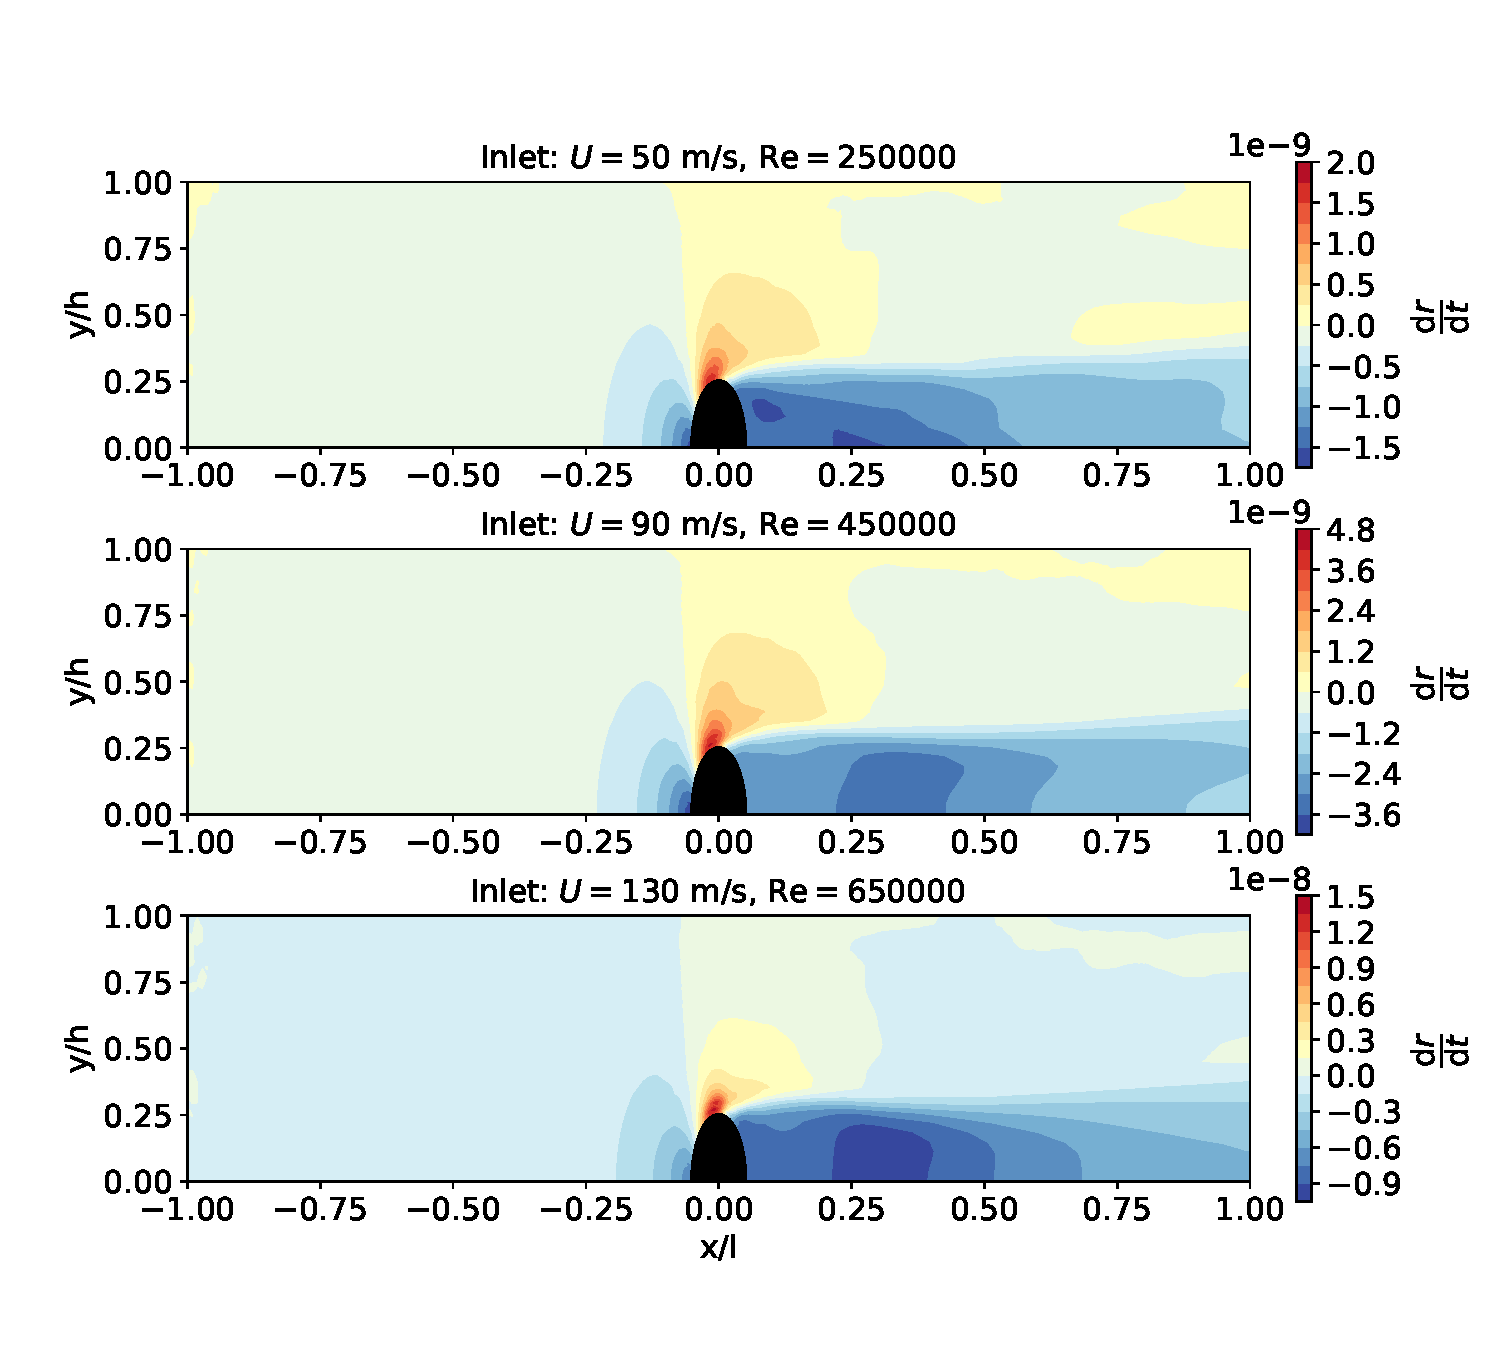
\includegraphics[trim={0 0 0 20},clip,width=1\textwidth]{Figures/drdt_plot_speed_compare.pdf}
    \caption{Droplet growth rate contour for different inlet velocity conditions}
    \label{f:Mass_Fraction_het}
\end{figure}
\subsection{Mass Fraction Progression for Flat Plate Case}
\begin{figure}[H]
    \centering
    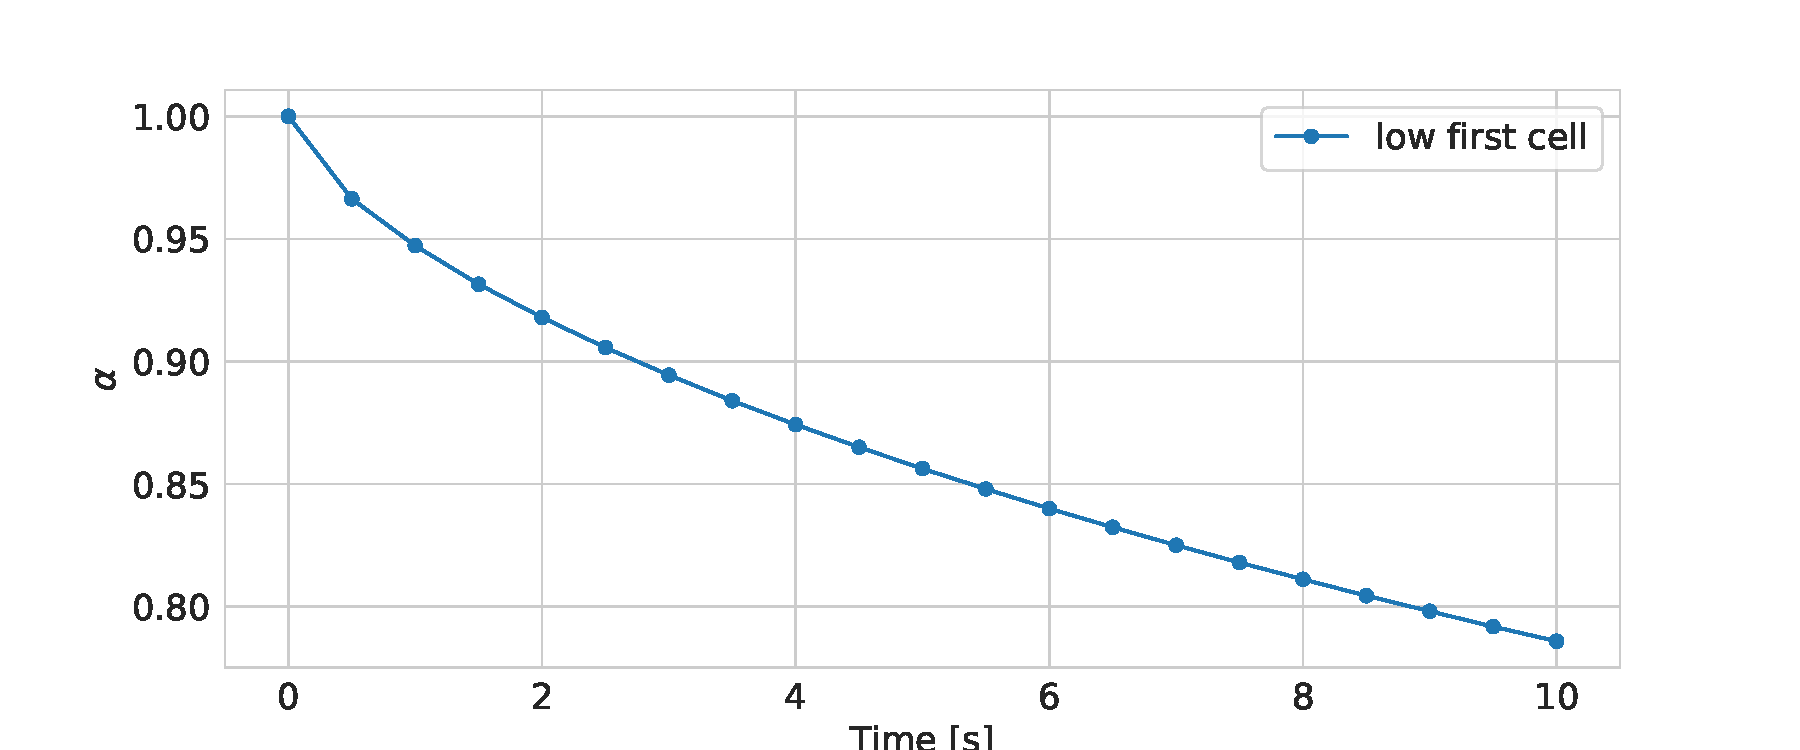
\includegraphics[trim={0 0 0 20},clip,width=1\textwidth]{Figures/mass_fraction_time_progression.pdf}
    \caption{Time progression of the mass fraction, $\alpha$, in the flat plate case. Saturation Temperature is $T'=303\mathrm{K}$ and first height is $20\mathrm{mm}$.}
    \label{f:Mass_Fraction_het}
\end{figure}
\section{Thermophysical Properties}\label{s:appendix B}
\begin{table}[H]
    
    \centering
    % \captionsetup{justification=centering}
    \caption{Calculation of water liquid and vapor properies}
    \renewcommand{\arraystretch}{2}
    \begin{tabular}{||c|c||}
        
    \hline
    \textbf{Variable} & \textbf{Fitting equations} \\ \hline\hline
    Vapor thermal conductivity \cite{Sutherlands_law} $\lambda_{v}\: \mathrm{[W/mK]}$     &      $0.0181\left(\frac{T}{300}\right)^{1.5}\cdot\frac{2550}{T+2200}$           \\\hline
    Air thermal conductivity \cite{Sutherlands_law} $\lambda_{a}\: \mathrm{[W/mK]}$     &      $0.0241\left(\frac{T}{273}\right)^{1.5}\cdot\frac{461}{T+194}$           \\\hline
    Vapor dynamic viscosity \cite{Sutherlands_law} $\mu_{v}\:\mathrm{[Pa\:s]}$      &   $1.12\cdot10^{-5}\left(\frac{T}{350}\right)^{1.5}\cdot\frac{1414}{T+1064}$           \\\hline
    Air dynamic viscosity \cite{Sutherlands_law} $\mu_{a}\:\mathrm{[Pa\:s]}$      &   $1.716\cdot10^{-5}\left(\frac{T}{350}\right)^{1.5}\cdot\frac{384}{T+111}$           \\\hline
    Heat capacity \cite[T. 2-150]{doble2007perry} $c_{p,v/a}\:\mathrm{[J/kgK]}$      &   $C1+C2+\left(\frac{C3/T}{\sinh (C3/T)}\right)^{2}+C4\left(\frac{C5/T}{\cosh (C5/T)}\right)^{2}$           \\\hline
    Surface Tension \cite{doble2007perry} $\sigma\:\mathrm{[N/m]}$      &   $(75.83-0.1477(T-273))\cdot 10^{-3}$           \\\hline
    Mass diffusivity \cite{vCalc_2022} $\mathcal{D}\:\mathrm{[m^{2}/s]}$      &   $\frac{1.858\cdot 10^{-3}\cdot T^{1.5}\sqrt{1/M_{w}+1/M_{a}}}{p(0.5(\sigma_{1}+\sigma_{2}))^{2}\cdot \Omega}$           \\\hline
    Water specific gas constant \cite{doi:10.1021/ie4033999} $R\:\mathrm{[J/kgK]}$      &       CoolProp Python package         \\ \hline
    Latent heat \cite{doi:10.1021/ie4033999} $h_{vl}\:\mathrm{[kJ/kg]}$        &   CoolProp Python package                 \\ \hline
    Liquid density \cite{doi:10.1021/ie4033999} $\rho_{l}\:\mathrm{[kg/m^{3}]}$        &    CoolProp Python package               \\\hline
  
    \end{tabular}
    \label{t:perry_calcs}
\end{table}
\end{appendices}
\pagebreak
\end{document}